% !TeX spellcheck = en_US

% This is samplepaper.tex, a sample chapter demonstrating the
% LLNCS macro package for Springer Computer Science proceedings;
% Version 2.20 of 2017/10/04
%
\documentclass[runningheads]{llncs}
\usepackage{tikz}
\usepackage{graphicx}
\usepackage{comment}
\usepackage{multirow}
\usepackage{multicol}
\usepackage{xcolor}
\usepackage{amsmath}
\usepackage{amssymb}
\usepackage[linesnumbered,ruled,vlined]{algorithm2e}
%\usepackage{algorithm}
%For tiz figures self added
\usepackage{subcaption}

% \usetikzlibrary{positioning}
% \usepackage{xparse}
%\title{\section and \chapter}

%\setcounter{secnumdepth}{-1}
%\usepackage{hyperref}
\usepackage{bookmark}
\bookmarksetup{
  numbered,
  open
}


% Used for displaying a sample figure. If possible, figure files should
% be included in EPS format.
% If you use the hyperref package, please uncomment the following line
% to display URLs in blue roman font according to Springer's eBook style:
\renewcommand\UrlFont{\color{blue}\rmfamily}
\let\subparagraph\relax

\usepackage{titlesec}
\titleformat{\chapter}[display]
{\centering \normalfont\Large\bfseries}{\chaptertitlename\ \thesection}{12pt}{\large}


\begin{document}

%\title{Project Soteria\thanks{Supported by organization x.}}
%
% \titlerunning{Abbreviated paper title}
% If the paper title is too long for the running head, you can set
% an abbreviated paper title here
%
% \author{First Author\inst{1}\orcidID{0000-1111-2222-3333} \and
% Second Author\inst{2,3}\orcidID{1111-2222-3333-4444} \and
% Third Author\inst{3}\orcidID{2222--3333-4444-5555}}
% %
% \authorrunning{F. Author et al.}
% % First names are abbreviated in the running head.
% % If there are more than two authors, 'et al.' is used.
% %
% \institute{Princeton University, Princeton NJ 08544, USA \and
% Springer Heidelberg, Tiergartenstr. 17, 69121 Heidelberg, Germany
% \email{lncs@springer.com}\\
% \url{http://www.springer.com/gp/computer-science/lncs} \and
% ABC Institute, Rupert-Karls-University Heidelberg, Heidelberg, Germany\\
% \email{\{abc,lncs\}@uni-heidelberg.de}}
% %
%\maketitle              % typeset the header of the contribution
% %
% \begin{abstract}
% The abstract should briefly summarize the contents of the paper in
% 15--250 words.

% \keywords{First keyword  \and Second keyword \and Another keyword.}
% \end{abstract}


\setcounter{tocdepth}{50}
\tableofcontents

\renewcommand\thechapter{\arabic{chapter}}
%\addtocounter{chapter}{0}
%\setcounter{chapter}{0}

%\renewcommand\thechapter{7.5}

% !TeX root = ../sameplaper.tex
% !TeX spellcheck = en_US

\chapter{Lattices}
\setcounter{section}{0}


\section{Basics}
Lattices are the building blocks of lattice-based cryptography.
They find many applications in computer science and mathematics, including integer programming, diophantine approximation, cryptanalysis, the design of error-correcting codes for multi-antenna systems, and many more.
Currently, it is under prime focus among the cryptographic community due to its resistance towards attack by classical and quantum computers and some excellent properties that can be used to construct advanced cryptographic primitives, including fully homomorphic encryption, functional encryption, etc.

Lattices have been extensively used in cryptology in cryptanalysis (using lattice approximation algorithms to break cryptosystems) and in cryptography (using computationally hard lattice problems to design robust cryptographic schemes).
Furthermore, lattice-based encryption scheme enjoys solid security proofs based on worst-case hardness, relatively efficient implementations, and great simplicity.
Our primary focus here will be to discuss lattice primitives necessary to understand the practical aspects of lattice-based cryptography and homomorphic encryption and remain under this barrier.
For in-depth knowledge on lattices-based cryptography, exploration of survey paper \cite{peikert2016decade,nguyen2001two,micciancio2009lattice,peikert2016decade,regev2006lattice}, lecture notes \cite{MicciancioLN,regevlatticenotes,Vinodlatticenotes} and book \cite{MGbook} might be resourceful.

A lattice can be defined as the linear combinations with integer coefficients of the subgroup of any basis in $\mathbb{R}^n$.
More formally, it can be defined as
\begin{definition}
  Let $n\geq 1$ and let $\pmb{b}_1, \pmb{b}_2, \cdots, \pmb{b}_m$ be a basis of $\mathbb{R}^n$.
    The lattice with dimension $n$ and basis $\pmb{b}_1,\pmb{b}_2, \cdots, \pmb{b}_m$ is the set $\Lambda$ of all linear combinations of the basis vectors with integer coefficients:
    \begin{equation*}
        \Lambda(\pmb{b}_1,\cdots,\pmb{b}_m)=\mathbb{Z}\pmb{b}_1+\mathbb{Z}\pmb{b}_2+ \cdots + \mathbb{Z}\pmb{b}_m = \Big\{ \sum_{i=1}^{m} a_i\pmb{b}_i | a_1,a_2,\cdots,a_m \in \mathbb{Z} \Big\}
    \end{equation*}
\end{definition}
The basis vectors $\boldsymbol{b}_{1} ,\boldsymbol{b}_{2}, \cdots ,\boldsymbol{b}_{m}$ are said to be the generators of the lattice.
All bases have the same number of elements and are known as the $dimension$ of the lattice.
In this case, we have a lattice of $rank$ $m$ and $dimension$ $n$.
A lattice is said to be full rank when $n=m$.
In Figure \ref{fig:2ed_basis}, 2d-lattice generated by different basis vectors have been shown by Figure \ref{fig:1st_basis} and \ref{fig:2ed_basis} respectively.

The determinant of the lattice $\Lambda$ with basis $\pmb{b}_1, \pmb{b}_2, \cdots, \pmb{b}_n$ is defined as
\begin{equation*}
    det(\Lambda)=|det(\pmb{B})|
\end{equation*}

where $\pmb{B}$-- a $n\times n$ basis matrix with $\pmb{b}_i$ as its column.
Geometrically it corresponds to the inverse of the density of the lattice points in $\mathbb{R}^n$.
It is to be noted that the determinant of a lattice does not depend on the basis; another basis of the same lattice can be obtained by multiplying with an unimodular (determinant $\pm1$) matrix.


%https://cseweb.ucsd.edu/~daniele/papers/PostQuantum.pdf
%https://pure.tue.nl/ws/portalfiles/portal/47023806/719274-1.pdf
%https://cseweb.ucsd.edu/~daniele/papers/PostQuantum.pdf
%https://cseweb.ucsd.edu/classes/wi12/cse206A-a/lec1.pdf
%https://web.cs.ucla.edu/~nmanohar/nmanohar_files/UndergradThesis.pdf
When we study lattices, often we come across dual of a lattice, a dual of a lattice $\Lambda$ in $\mathbb{R}^n$ denoted by $\Lambda^{*}$ is defined as %the set of all vectors $\pmb{y} \in \mathbb{R}^n$ that satisfies
\begin{equation*}
    \Lambda^{*} =\{ \pmb{y} \in \mathbb{R}^n \ |\ <\pmb{x}, \pmb{y}> \ \in\ \mathbb{Z} \ \text{ for all vectors } \pmb{x} \in \Lambda \}
\end{equation*}
In general,
\begin{equation*}
    \Lambda^{*} =\{ \pmb{y} \in \text{span}(\Lambda) \ |\ <\pmb{x}, \pmb{y}> \ \in\ \mathbb{Z} \ \text{ for all vectors } \pmb{x} \in \Lambda \}
\end{equation*}

The lattice of integer points satisfies $(\mathbb{Z}^n)^* = \mathbb{Z}^n$ (and hence it is also addressed by self-dual).
Similarly, $(2\mathbb{Z}^n)^* =\frac{1}{2}\mathbb{Z}^n$.
It can be shown that for any basis $\pmb{B} \in \mathbb{R}^{n\times n}$, $\Lambda(\pmb{B})^{*} = \Lambda((\pmb{B}^{-1})^T)$.
From this it follows that $det(\Lambda^{*}) = \frac{1}{det(\Lambda)}$.


We often come across $q$-ary lattices in lattice cryptography and homomorphic encryption.
These are the lattices $\Lambda$ satisfying $q\mathbb{Z}^n \subseteq \Lambda \subseteq \mathbb{Z}^n$ for some (possibly prime) integer $q$.
This can also be understood as the lattice $\Lambda$ where the membership of a vector $\boldsymbol{x}$ in $\Lambda$ is determined by $\boldsymbol{x}$ mod $q$.
$q$-ary lattices are in one-to-one correspondence with linear codes in $\mathbb{Z}^n_q$.
In lattice cryptography, most constructions use $q$-ary lattices as their hard-on-average problem.
We can also say that any integer lattice $\Lambda \subseteq \mathbb{Z}^n$ is a $q$-ary lattice for some $q$, whenever $q$ is an integer multiple of the determinant $det(\Lambda)$.
However, in cryptographic applications, $q$ is usually kept much smaller than $det(\Lambda)$.

Given a matrix $\pmb{A} \in \mathbb{Z}^{n\times m}$ for parameters $q,m$ and $n$, we can define q-ary lattices as
\begin{align*}
    \Lambda_q(\pmb{A})         & = \{\pmb{y} \in \mathbb{Z}^m : \pmb{y = A^Ts} \text{ mod q for some } \pmb{s} \in \mathbb{Z}^n \} \\
    \Lambda^{\perp}_q(\pmb{A}) & = \{\pmb{y} \in \mathbb{Z}^m : \pmb{Ay = 0} \text{ mod }q \}
\end{align*}

In the definition above first $q$-ary lattice is generated by the rows of matrix $\pmb{A}$. In contrast, the second $q$-ary lattice contains all orthogonal vectors with respect to rows of $\pmb{A}$ modulo $q$.
It is clear from the dual definition above that these two lattices are dual to each other up to normalization, namely,
$\Lambda^{\perp}_q(\pmb{A}) = q \cdot \Lambda_q(\pmb{A})^{*}$ and
$\Lambda_q(\pmb{A}) = q \cdot \Lambda^{\perp}_q(\pmb{A})^{*}$.
%https://cseweb.ucsd.edu/~daniele/papers/PostQuantum.pdf


Fundamental parallelepiped generated by the basis matrix $\pmb{B}$ is defined as
\begin{align*}
    P(\pmb{B}) & =\{\pmb{Bx} \ | \ \pmb{x} \in [0,1)^n\}
\end{align*}
%https://ocw.mit.edu/courses/18-409-topics-in-theoretical-computer-science-an-algorithmists-toolkit-fall-2009/a5351bd811ac52366dec759f2c6b2fac_MIT18_409F09_scribe18.pdf

%http://www.cs.umd.edu/~gasarch/BLOGPAPERS/RegevLWEtalk.pdf
%https://eprint.iacr.org/2012/533.pdf






%--------------lattice figure-----------------------
\begin{figure}[h!]
    \centering
    \begin{subfigure}[t]{0.48\textwidth}
        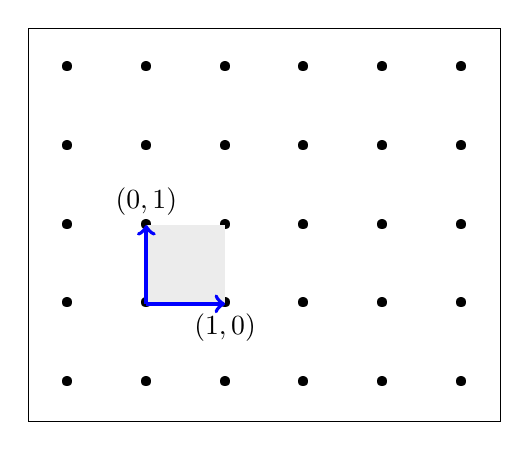
\begin{tikzpicture}
            \draw[color=black] (-3.5,3.5) -- (2.5,3.5) -- (2.5,-1.5) -- (-3.5,-1.5) --  (-3.5,3.5);
            \foreach \Point in {(-3,3), (-3,2), (-3,1), (-3,0), (-3,-1),
                    (-2,3), (-2,2), (-2,1), (-2,0), (-2,-1),
                    (-1,3), (-1,2), (-1,1), (-1,0), (-1,-1),
                    (0,3),  (0,2),  (0,1),  (0,0),  (0,-1),
                    (1,3),  (1,2),  (1,1),  (1,0),  (1,-1),
                    (2,3),  (2,2),  (2,1),  (2,0),  (2,-1)}{
                    \node at \Point {\textbullet};
                }
            \fill [color=gray!15] (-2,0) rectangle (-1,1);
            \draw[->, thick, line width=.5mm,  blue] (-2,0)--(-2,1); % l'axe des abscisses
            \draw[->, thick, line width=.5mm,  blue] (-2,0)--(-1,0); % l'axe des ordonnées
            \node at (-2,1.3) {$(0,1)$};
            \node at (-1,-.3) {$(1,0)$};

        \end{tikzpicture}
        \caption{Basis in 2d lattice}
        \label{fig:1st_basis}
    \end{subfigure}\quad%
    \begin{subfigure}[t]{0.48\textwidth}
        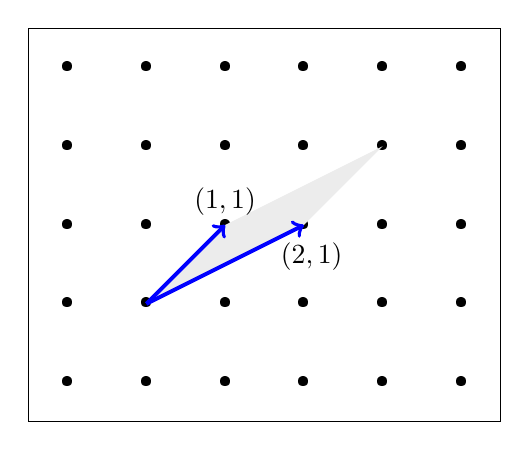
\begin{tikzpicture}
            \draw[color=black] (4.5,3.5) -- (10.5,3.5) -- (10.5,-1.5) -- (4.5,-1.5) --  (4.5,3.5);
            \foreach \Point in {(5,3), (5,2), (5,1), (5,0), (5,-1),
                    (6,3), (6,2), (6,1), (6,0), (6,-1),
                    (7,3), (7,2), (7,1), (7,0), (7,-1),
                    (8,3), (8,2), (8,1), (8,0), (8,-1),
                    (9,3), (9,2), (9,1), (9,0), (9,-1),
                    (10,3), (10,2), (10,1), (10,0), (10,-1)}{
                    \node at \Point {\textbullet};
                }
            \fill[color=gray!15] (6,0) -- (8,1) -- (9,2) -- (7,1) --  (6,0);
            \draw[->, thick, line width=.5mm,  blue] (6,0)--(7,1); % l'axe des abscisses
            \draw[->, thick, line width=.5mm,  blue] (6,0)--(8,1); % l'axe des ordonnées
            \node at (7,1.3) {$(1,1)$};
            \node at (8.1,.6) {$(2,1)$};

        \end{tikzpicture}
        \caption{Another basis in the same lattice}
        \label{fig:2ed_basis}
    \end{subfigure}
    \caption{Figure \ref{fig:1st_basis} shows the lattice generated by $(1,0)$ and $(0,1)$ in $\mathbb{Z}^2$, it is the lattice of all integers points in $\mathbb{Z}^2$.
        However, this is not unique and can also be generated as shown in the figure\ref{fig:2ed_basis} with $(1,1)$ and $(2,1)$.
        Similarly, Yet another example of basis in $\mathbb{Z}^2$ can be generated by $(2021, 1)$ and $(2022, 1)$.
        However, it is to be noted that $(1, 1)$ and $(2,0)$ are not a basis of $\mathbb{Z}^2$; this is because it only generates the lattice of all integer points whose coordinates sum to an even number.
        All examples mentioned so far are full-rank lattices.
        An example of a lattice that is not full is $\Lambda((2, 1))$. It is of rank one and dimension 2.
        A one-dimensional lattice of full-rank is the lattice $\mathbb{Z}= \Lambda((1))$.}
    \label{fig:Basis_of_2d_lattice}
\end{figure}
%-----------Figure ends here---------------


In Figure \ref{fig:Basis_of_2d_lattice}, fundamental parallelepiped $P(\pmb{B})$ is shown by the gray-shaded region.
Note that $P(\pmb{B})$ not only depends on the lattice but also on the choice of the basis $\pmb{B}$.
A basis is termed a `good' or a `bad' based on the type of parallelepiped it forms.
A good basis is the one that forms a square-like parallelepiped, while a `bad' basis is the one that creates a very thin parallelepiped as shown by Figure \ref{fig:1st_basis} and \ref{fig:2ed_basis} respectively.

%https://eprint.iacr.org/2012/533.pdf
%https://web.cs.ucla.edu/~nmanohar/nmanohar_files/UndergradThesis.pdf
In lattice, there are several hard problems.
The conjectured intractability of such problems is central to constructing secure lattice-based cryptosystems.
The most common ones include the following:

\begin{definition}
    Shortest Vector Problem (SVP): Given a lattice basis, the problem is to find the shortest non-zero vector present in the lattice.
    Mathematically, given a lattice basis $\pmb{B}\in \mathbb{Z}^{m \times n}$, find a nonzero lattice vector $\pmb{Bx}$, $\pmb{x}\neq \pmb{0}, \pmb{x} \in \mathbb{Z}^n$, such that $||\pmb{Bx}|| \leq ||\pmb{By}||$, $\forall \pmb{y} \in \mathbb{Z}^n$.%and $\pmb{y} \neq \pmb{0}$.
\end{definition}
In practice, the length of the shortest non-zero vector present in a lattice $\Lambda$ is denoted by $\lambda_1(\Lambda)$ and $i^{th}$ successive minimum by $\lambda_i(\Lambda)$.
The $i$-th successive minimum $\lambda_i(\Lambda)$ is the radius $r$ of the smallest $n$-dimensional (Euclidean) ball that contains $i$ linearly independent vectors in $\Lambda$.
Mathematically,
\begin{equation*}
    \lambda_i(\Lambda) = min\{r > 0 | dim(span(\Lambda \cap rU)) \geq i\}
\end{equation*}
where U is the unit ball in the Euclidean norm \cite{laarhoven2012solving}.

%https://eprint.iacr.org/2016/146.pdf
An $n$-dimensional Euclidean ball of radius $R$ denoted by $Ball_n(R)$ has a volume of
\begin{equation*}
    V_n(R) = R^n \frac{\pi^{n/2}}{\Gamma(n/2+1)}
\end{equation*}
where Stirling's approximation yields $\Gamma(n/2+1) \approx \sqrt{\pi n}(n/2)^{n/2}e^{-n/2}$ and $V_n(1)^{-1/n} \approx \sqrt{n/(2\pi e)} \approx \sqrt{n/17}$

The Gaussian Heuristic approximates the number of lattice points in a continuous (usually convex and symmetric) set $S\subset R^n$.
To be more precise, it says that for a given set $S$ and a lattice $\Lambda$, we get $|S\cap \Lambda| \approx vol(S)/det(\Lambda)$.

Considering $S$ as the origin-centered ball of radius $R$, the number of lattice points is approximately $V_n(R)/vol(\Lambda)$, Thus the length of shortest vector $\lambda_1$ in a ball of radius $R$ is
\begin{equation*}
    \lambda_1(\Lambda) \approx det(\Lambda)^{1/n}/ V_n(1)^{1/n}= \frac{(\Gamma(n/2+1)det(\Lambda))^{1/n}}{\sqrt{\pi}}
\end{equation*}
%This is called the Gaussian heuristic of a lattice and is denoted by $GH(\mathcal{L})=det(\mathcal{L})^{1/n}/ V_n(1)^{1/n}$

%Gaussian heuristic suggests that the shortest vector in a lattice $L$ of rank $m$ has Euclidean norm about $\frac{1}{\sqrt{\pi}} \Gamma(1+\frac{m}{2})^{1/m} Vol(\mathcal{L})^{1/m}$,
which is approximately $\sqrt{\frac{n}{2\pi e}} Vol(\Lambda)^{1/n}$.
In a $q$-ary lattice $\Lambda$ (of rank $m$), this is $\sqrt{\frac{m}{2\pi e}}q^{(m-n)/m}$.
A $q$-ary lattices contain known vectors of Euclidean length equal to $q$.
Hence, an estimate of the Euclidean length of known short vectors is

\begin{equation}
    \lambda_1(\Lambda) \approx min \Big\{q,\sqrt{\frac{m}{2\pi e}} q^{\frac{m-n}{m}} \Big\}
\end{equation}

%\lambda_2(L') \approx

\begin{comment}


In contrast, the vector $\pmb{e}$ has Euclidean length around $\sqrt{m}\delta$
on average and so the vector $(\frac{e}{M})$ has length approximately $\sqrt{2m}\sigma$ when $M = \sqrt{m}\sigma$.
In our experiments we take $M = 1$ and so assume that $\lambda_1(L') \approx \sqrt{m}\sigma$.
Hence the gap is
\begin{equation}
    \gamma(m) = \frac{\lambda_2(L')}{\lambda_1(L')} \approx \frac{min\{q,\frac{1}{\sqrt{\pi}} \Gamma(1+\frac{m}{2})^{\frac{1}{m}}q^{\frac{m-n}{m}}}{\sqrt{m}\sigma} \approx \frac{min\{q, \sqrt{\frac{m}{2\pi e}}q^{\frac{m-n}{m}}\}}{\sqrt{m}\sigma}
\end{equation}
For a successful attack we want this gap to be large, so we will need
\begin{equation}
    \sigma << q^{\frac{m-n}{m}} < \frac{q}{\sqrt{m}}
\end{equation}

To determine whether an LWE instance can be solved using the embedding technique and a lattice reduction algorithm with a given (root) Hermite factor $\delta$, one can choose a suitable subdimension $m$ and verify that the corresponding gap satisfies the condition $\gamma = \gamma(m) > c\delta^m$ for a suitable value $c$.
Since the constant $c$ is unknown, we can maximize $min{q, q^{\frac{m-n}{m}}}/\delta^m$ for fixed $n$, $q$, $\delta$ to get the ``optimal” sub-dimension (which maximizes the success probability of the algorithm) to be
\begin{equation}
    m = \sqrt{\frac{n\log{(q)}}{\log{(\delta)}}}
\end{equation}
where $\delta$ is the Hermite factor of the lattice basis reduction algorithm used.


It is to be noted that ISIS problem can be attacked by reducing it to CVP problem.
Considering a lattice $\mathcal{L}'= \Lambda^\perp_q(A^T)=\{ y \in \mathbb{Z}^m : A^Ty \equiv 0 (mod q)\}$, finds any vector (not necessarily short) $w \in Z^m$ such that $A^Tw \equiv v (mod q)$, then solves CVP for $(L', w)$ to find some $y$ close to $w$ and so returns $w-y$ as the ISIS solution.

We sketch the details of solving LWE (in the case of short secrets) by reducing
to ISIS and then solving by CVP.
Given $(A, b)$ we define $A' = (A|I_m)$ to get an ISIS instance $(A',b)$.
Choose any vector $w \in Z^{n+m}$ such that $A'w \equiv b$ (mod $q$).
Then the lattice $L' = \Lambda^{\perp}_q(A') = \{y \in Z^{n+m} : A'y \equiv 0 (\ mod\ q)\}$ is seen to have rank $m'=n+m$ and (assuming the rank of $A'$ is $n$) determinant $q^m = q^{m'-n}$ (the determinant condition can be seen by considering the index of the subgroup $qZ^{n+m}$ in the additive group $L'$).
The condition for success in the algorithm is $\sigma << q^{m/(n+m)}$.
Writing $m' = n+m$ this is $q^{(m'-n)/m'}$, which is the same as the LWE condition above
\end{comment}




\begin{definition}
    Closest Vector Problem (CVP): Given a lattice basis and a target vector (not necessarily from the lattice), the problem is to find a lattice vector in the given lattice closest to the target vector.
    Mathematically, given a lattice basis $\pmb{B}\in \mathbb{Z}^{m \times n}$ and a target vector $\pmb{t} \in \mathbb{Z}^m$, the problem is to find a lattice vector $\pmb{v}=\pmb{Bx}$ for some $\pmb{x} \in \mathbb{Z}^n$, such that $||\pmb{v}-\pmb{t}|| \leq ||\pmb{By}-\pmb{t}||$ for all $\pmb{y} \in \mathbb{Z}^n$
\end{definition}

\begin{definition}
    Shortest Independent Vectors Problem (SIVP): Given a lattice basis, the problem is to find $n$ (dimension of the lattice) linearly independent lattice vectors with minimum length (Euclidean norm).
    Alternatively, it asks for a new basis that yields the same lattice but with a minimum length of the longest vector.
    Mathematically, given a lattice basis $\pmb{B}\in \mathbb{Z}^{m \times n}$, find lattice vectors $\pmb{Bx}_1, \cdots, \pmb{Bx}_n \in \mathbb{Z}^m$, $\pmb{x}_1,\cdots,\pmb{x}_n \in \mathbb{Z}^n$ that are linearly independent and $||\pmb{Bx}_i|| \leq \lambda_n(\Lambda (\pmb{B})$ for $1 \leq i \leq n$.
\end{definition}

In literature, besides the above problems, the Shortest Integer Solution (SIS) problem finds many applications, including its use in solving LWE.
The SIS problem is defined as

\begin{definition}Short Integer Solution (SIS) problem:
    Given a $q$-ary lattice, the problem is to find an orthogonal vector with a restricted norm.
    Formally, given a lattice basis generated by integer matrix $\pmb{A}^{m \times n}$ (where typically $m$ is much bigger than $n$) and an integer modulus $q$ the problem is to find a vector $\pmb{y}$, $0<||\pmb{y}||\leq \beta$ if it exists, such that $\pmb{A}^T\pmb{y} \equiv 0 \ ( \text{mod} \ q)$.
    %$\pmb{y} \in \pmb{B}$ a set of vectors that are “short” in some sense (e.g., $\pmb{B} = \{-1,0,1\}^m$), with $||\pmb{y}||\leq \beta$ if it exists, such that $\pmb{A}^T\pmb{y} \equiv 0 \ ( \text{mod} \ q)$.

    A variant of this problem is known as the inhomogeneous SIS problem (ISIS), where given $\pmb{A}$ and $\pmb{v}$ find $\pmb{y}$,
    % \in \pmb{B}$,
    $0<||\pmb{y}||\leq \beta$ if it exists, such that $\pmb{A}^T\pmb{y} \equiv \pmb{v} \ ( \text{mod} \ q)$.
\end{definition}

A solution to the ISIS problem gives a value for the error $\pmb{e}$ and can be used to solve the LWE problem.
However, we need to rephrase the LWE problem into the ISIS problem.
There are two ways to rephrase the LWE problem into the ISIS problem in the literature mentioned in \cite{bai2014lattice} and \cite{micciancio2011pseudorandom}, respectively.

Bai and Galbraith’s \cite{bai2014lattice} way of rephrasing the LWE problem into an ISIS problem goes as follows: given $(\pmb{A}, \pmb{b} \equiv \pmb{As} + \pmb{e}$ (mod $q$)) one can form the ISIS instance as
\begin{equation*}
    (\pmb{A} | \pmb{I}_m)
    \begin{pmatrix}
        \pmb{s} \\
        \pmb{e}
    \end{pmatrix}
    \equiv b \ (\text{mod} \ q)
\end{equation*}
where $I_m$ is the $m \times m$ identity matrix.

Micciancio and Mol present an alternative way of transforming the LWE problem into an ISIS problem in \cite{micciancio2011pseudorandom}.
The technique is to construct a matrix $\pmb{G} \in \mathbb{Z}^{(m-n)\times m}_q$ such that $\pmb{GA} \equiv 0$ (mod $q$).
Thus the LWE problem ($\pmb{A}$, $\pmb{b}$) gets transformed into the ISIS instance as ($\pmb{G},\pmb{Gb}\equiv \pmb{Ge}$ (mod $q$)).
More detail about the same can be obtained in lemma 9 and 10 of \cite{micciancio2011pseudorandom}.


It is to be noted that both approaches are equivalent when the secret vector $\pmb{s}$ is chosen from the error distribution.
However, when the secret vector $\pmb{s}$ is chosen from a ``small" distribution, the earlier approach is better than the latter one.
This is because the reduction eliminates the vector s. Thus the advantage of the secret $\pmb{s}$ being ``small'' compared with $\pmb{e}$ no longer can be used.


%Remark: we usually consider Euclidean norm however any norm it should work.
%\textbf{Geometric Series Assumption}

An approximate variant of the above problems is often considered in lattice cryptography.
Approximate variants are denoted by an additional parameter $\gamma$ as a subscript, usually indicating the approximation factor.
For instance, in $SVP_\gamma$ the goal is to find a vector whose norm is at most $\gamma$ times that of the shortest nonzero vector present in the lattice.
It is to be noted that lattice problems can be defined for any norm, but in practice, Euclidean norm $||\pmb{x}||=\sqrt{\sum_i x^2_i}$ is the most common one \cite{peikert2008limits}.

\section{Lattice reduction}
Lattice reduction algorithms are used to convert a bad basis into a good basis \cite{laarhoven2012solving}.
Working on a good basis, viz., finding a short vector, is comparatively easier than working on a bad basis.
Thus bad basis is converted into a good basis for practical lattice attacks and is done by lattice reduction algorithms.
Alternatively, lattice reduction plays a central step in breaking hard lattice problems.
Hence without reviewing lattice reduction algorithms explaining lattice attacks on hard lattice problems will be incomplete.
Thus in the following few pages, we will briefly discuss the different lattice reduction algorithms from the literature.


Using lattice reduction viz., BKZ, Schnorr in \cite{schnorr2003lattice} introduced the geometric series assumption (GSA) to find the Gram-Schmidt length ($||\pmb{b}_i^*||$) of BKZ-reduced basis.
It says that the BKZ-reduced basis decay geometrically with quotient $r$ for $i = 1,\cdots,n$, viz.,
\begin{equation*}
    ||\pmb{b}_i^*||^2/||\pmb{b}_1||^2=r^{i-1} \hspace{2em} for \ some \ r \in [3/4,1)
\end{equation*}
$r$ here represents the GSA constant.


%--------------start lattice relation figure-----------------------
\begin{figure}[h!]
    \centering
    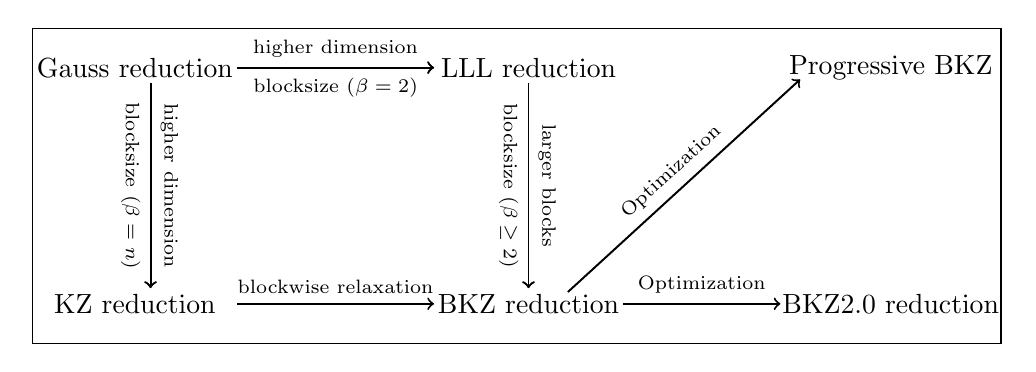
\begin{tikzpicture}
        %box drawing
        \draw[color=black] (-6.3,.5) -- (6,.5) -- (6,-3.5) -- (-6.3,-3.5) --  (-6.3,.5);
        % horizental
        \draw[->, line width=.25mm,  black] (-3.7,0)--(-1.2,0) node[midway,above,font=\scriptsize] {higher dimension};
        \draw[->, line width=.25mm,  black] (-3.7,0)--(-1.2,0)  node[midway,below,font=\scriptsize] {blocksize ($\beta=2)$};

        %Curved
        \draw[->, line width=.25mm,  black] (.5,-2.85)--(3.45,-.15) node[midway,above,font=\scriptsize,sloped] {Optimization};


        \draw[->, line width=.25mm,  black] (-3.7,-3)--(-1.2,-3) node[midway,above,font=\scriptsize] {blockwise relaxation};
        \draw[->, line width=.25mm,  black] (1.2,-3)--(3.2,-3) node[midway,above,font=\scriptsize] {Optimization};

        % Vertical
        \draw[->, line width=.25mm,  black] (-4.8,-.2)--(-4.8,-2.8) node[midway,above,font=\scriptsize,sloped] {higher dimension};
        \draw[->, line width=.25mm,  black] (-4.8,-.2)--(-4.8,-2.8) node[midway,below,font=\scriptsize,sloped] {blocksize ($\beta=n$)};

        \draw[->, line width=.25mm,  black] (0,-.2)--(0,-2.8) node[midway,above,font=\scriptsize,sloped] {larger blocks};
        \draw[->, line width=.25mm,  black] (0,-.2)--(0,-2.8) node[midway,below,font=\scriptsize,sloped] {blocksize ($\beta \geq 2)$};


        \node at (-5,0) {Gauss reduction};
        \node at (0,0) {LLL reduction};
        \node at (-5,-3) {KZ reduction};
        \node at (0,-3) {BKZ reduction};
        \node at (4.6,-3) {BKZ2.0 reduction};
        \node at (4.6,0) {Progressive BKZ};
    \end{tikzpicture}
    \caption{Overview of the basis reduction algorithms.} %(Picture taken from \cite{laarhoven2012solving})}
    \label{fig:lattice_relations}
\end{figure}
%--------------end lattice relation figure-----------------------

Lattice reduction algorithms can be viewed as a hierarchy of BKZ algorithms based on the block parameter $k$ used for the lattice reduction as shown in Figure \ref{fig:lattice_relations}.
When $k=2$, the BKZ algorithms run in polynomial time, but the reduced basis will only be LLL-reduced-- producing short vectors within exponential factors of a short vector.
When $k=n$, the reduced lattice is KZ (Korkine-Zolotarev) reduced or HKZ (Hermite-Korkine-Zolotarev) reduced -- this is in some way optimally reduced but takes exponential run time.
Thus usually, lattice reduction is performed based on intermediate block size, which is decided based on the required root Hermite factor (discussed below).
When optimization is used to optimize the BKZ algorithm's run time, it gives rise to BKZ2.0.
Further optimization to the BKZ is known as the Progressive BKZ, as shown in Figure \ref{fig:lattice_relations}.

Gama and Nguyen \cite{gama2008predicting} provided a heuristic to estimate the shortest vector produced by lattice reduction algorithms.
Suppose a lattice reduction algorithm is fed with a basis of a lattice $\Lambda$ of dimension $n$, then the algorithm outputs a list of vectors $\pmb{b}_1,\pmb{b}_2,\cdots,\pmb{b}_n$.
The shortest vector produced by the lattice reduction algorithm can be approximated using the root Hermite factor, denoted by $\delta_0$, as defined in \cite{gama2008predicting} as

% Hermite factor is used to determine the quality of basis produced by a lattice reduction algorithm and is usually denoted by $\delta_0$. A Hermite factor is defined as the shortest non-zero vector $\textbf{b}_0$ produced by the lattice reduction algorithm and is represented as
\begin{equation}
    ||\pmb{b}_0||=\delta^n_0 \cdot \text{vol}(\Lambda)^{1/n}
    \label{eq:first_min}
\end{equation}
%https://eprint.iacr.org/2013/839.pdf
Considering $m$ samples in a $q$-ary lattice the expression \ref{eq:first_min} above simplifies to
\begin{equation*}
    ||\pmb{b}_0|| \approx \delta^m_0 \cdot \text{vol}(\Lambda)^{n/m}
\end{equation*}
with high probability, where $n$ is the LWE dimension and $m$ is the number of samples under consideration.
The minimum of the expression above is attained for $m=\sqrt{\frac{n\log{q}}{\log \delta_0}}$ \cite{Micciancio2009}.

LLL algorithm produces $\delta = 1.021$.
Gama and Nguyen in \cite{gama2008predicting} argued that $\delta = 1.01$ is about the limit of practical algorithms (i.e., variants of BKZ using extreme pruning and large block size).
Chen and Nguyen in \cite{chen2011bkz} extended this analysis to algorithms with greater running time.
Their heuristic argument is that a Hermite factor corresponding to $\delta = 1.006$ might be reachable with an algorithm performing around $2^{110}$ operations.

Gama and Nguyen in \cite{gama2008predicting} focus on the unique-SVP problem.
One seeks a short vector in a lattice $\Lambda$ when one knows that there is a significant gap $\gamma = \lambda_2(\Lambda)/\lambda_1(\Lambda)$, where $\lambda_i(\Lambda)$ denotes the $i$-th successive minima of the lattice.
The unique SVP problem arises when solving CVP using the embedding technique.
The standard theoretical result is that if one uses a lattice reduction algorithm with Hermite factor $\delta$, the algorithm outputs the shortest vector if the lattice gap satisfies $\gamma > \delta^{2m}$.
However, Gama and Nguyen observe that practical algorithms will succeed as long as $\gamma > c\delta^m$ for some small constant $c$ (they provided values of $c = 0.26$ and $c = 0.45$ for different families of lattices).
Later, Luzzi, Stehl\'e, and Ling \cite{luzzi2013decoding} provided some theoretical justification claiming that the unique-SVP problem is easier to solve when the gap is significant.

Below we have briefly discussed different lattice reduction algorithms available in the literature with their run time and available implementations.




\subsection{Gauss Algorithm}
Gauss algorithm \cite{bremner2011lattice} (sometimes also attributed to Lagrange \cite{de1773recherches}) finds an optimally reduced basis in a two-dimensional lattice.
The optimally reduced basis $\{\pmb{b}_1,\pmb{b}_2\}$ in a $2$-dimensional lattice $\Lambda$ are such that $||\pmb{b}_1||=\lambda_1(\Lambda)$ and $||\pmb{b}_2||=\lambda_2(\Lambda)$.

%In this algorithm, we assume that at any point, the Gram-Schmidt coefficient µ2,1 = (b2 ·b1)/kb1k two is known and up to date with respect to the current vectors b1 and b2. For simplicity and to focus on the high-level description rather than the low-level details, in the algorithms discussed in this section we will omit details on updating the GSO-vectors b∗i and the coefficients µi, j.

The algorithm works as follows: in each iteration, the algorithm checks $||\pmb{b}_1|| \geq ||\pmb{b}_2||$.
If the condition evaluates to be true, then it swaps the vectors and subtract the shorter vector $\pmb{b}_1$ multiplied with integral multiple of $(\lfloor\mu_{2,1}\rceil = \lfloor \frac{(\pmb{b}_1 \cdot \pmb{b}_2)}{||\pmb{b}_1||^2}\rceil)$ from the longer vector $\pmb{b}_2$ to obtain a shorter vector $\pmb{b}_2 \leftarrow \pmb{b}_2 - \lfloor \mu_{2,1}\rceil\pmb{b}_1$ then it swaps the vectors $\pmb{b}_1$ and $\pmb{b}_2$.
The algorithm stops when the condition $||\pmb{b}_1|| \geq ||\pmb{b}_2||$ fails.
The algorithm upon completion produces $|\mu_{2,1}| \leq \frac{1}{2}$

The algorithm runs in poly($\log{||\pmb{B}||}$) time i.e.
in time polynomial in the size of the input basis $\pmb{B}$.






\subsection{LLL Algorithm}
LLL algorithm acronym of its designers name Lenstra-Lenstra-Lov\'{a}sz \cite{lenstra1982factoring} is the generalization of Gauss Algorithm\cite{bremner2011lattice} presented above to the higher dimension.
Extending the Gauss algorithm to the higher dimension may seem easy, but it's not.
This is due to the size-reduction and the swapping step; there are too many basis vectors to choose from, and one needs a procedure to make this choice.
It is finally achieved by imposing the following two conditions:
\begin{enumerate}
    \item $|\mu_{i,j}|\leq \frac{1}{2}$  \hspace{11.2em} for $0 \leq j < i \leq n-1$
    \item $||\pmb{v}_i^* + \mu_{i,i-1}\pmb{v}_{i-1}^*||^2 \geq \alpha ||\pmb{v}_{i-1}^*||^2$ \hspace{1.8em} for $2\leq i \leq n$
\end{enumerate}

%In two dimensional lattice, the lattice vectors $\{\pmb{v}_1,\pmb{v}_2\}$ is minimized by repeatedly performing swapping operation based on $||\pmb{v}_1|| \leq ||\pmb{v}_2||$ after performing $\pmb{v}_2=\pmb{v}_2-\lceil \frac{\pmb{v}_2 \cdot \pmb{v}_1}{\pmb{v}_1 \cdot \pmb{v}_1} \rfloor \pmb{v}_1$ until no further change can be made.
The minimal basis obtained by performing the above operations satisfies the inequality $ \mu_{2,1}=\frac{\pmb{v}_2 \cdot \pmb{v}_1}{\pmb{v}_1 \cdot \pmb{v}_1}\leq \frac{1}{2}$.



The first condition is known as Lov\'asz condition, and the second condition is known as the exchange condition.
Here $\alpha$ ($\frac{1}{4}<\alpha<1 $) represents the reduction parameter and $\pmb{v}^*_1,\pmb{v}^*_2,\cdots,\pmb{v}^*_n$ represents the orthogonal vector obtained using Gram-Schmid Orthogonalization \cite{lang2012introduction}.
As $\pmb{v}^*_1,\pmb{v}^*_2,\cdots,\pmb{v}^*_n$ are orthogonal to each other, exchange condition also evaluates to
\begin{enumerate}
    \item[$2'.$] $||\pmb{v}_i^*||^2 \geq (\alpha-\mu_{i,i-1}^2) ||\pmb{v}_{i-1}^*||^2$ \hspace{1.8em} for $2\leq i \leq n$
\end{enumerate}

In brief, the LLL algorithm works by size reduction of basis vectors pairwise followed by Lov\'asz condition checking to confirm if the Lov\'asz condition still holds; if it does not, then it performs the vector swap operation between the current vector to that of the previous vector.
More detail about the LLL algorithm can be obtained in section 4.3 of \cite{bremner2011lattice}.

There are many variants of the original LLL algorithm available in the literature.
One of the well-known variants is the LLL by deep
insertions, proposed by Schnorr and Euchner \cite{schnorr1994lattice}.
The idea is to rather than swapping two neighboring basis vectors $\pmb{b}_i$ and $\pmb{b}_{i-1}$; this algorithm inserts $\pmb{b}_i$ somewhere in the basis, at some position $j<i$.
In short, this further generalizes the original LLL algorithm since taking $ j=i-1 $ for each swap leads to the original LLL algorithm.
The position of insertion of vector $\pmb{b}_i$ is decided based on the smallest index $j$ that gains a factor of at least $\delta$, same as that of proof of the LLL algorithm.
This slight modification in the original LLL leads to shorter vectors with a longer run time.

LLL algorithm runs in polynomial time \cite{bremner2011lattice}, given a rank $m$ integer lattice with basis vectors of Euclidean norm less than $\pmb{B}$ in an $n$-dimensional space, the LLL algorithm outputs a reduced basis in time $O(m^3n \log{\pmb{B}}\cdot M(m\log{\pmb{B}}))$ bit operations, where $M(k)$ represents the multiplication time of $k$-bit integers.
Presence of $m$ and/or $\log{\pmb{B}}$ makes the worst-case time complexity of the original LLL algorithm relatively high for applications where they are significantly large.
To reduce computational complexity, Nguyen and Stehl\'e proposed a variant of the LLL algorithm in \cite{nguyen2009lll}, that has a run time of $O(m^2n(m+\log{\pmb{B}}) \log{\pmb{B}}\cdot M(m))$.
In \cite{chen2011bkz}, Chen and Nguyen performed modification to the fplll\cite{cade2008fplll}, using \cite{novocin2011lll} and reported a heuristic run time of the LLL algorithm as $O(n^3\log^2\pmb{B})$.

In the original LLL paper \cite{lenstra1982factoring}, it has been reported that theoretically, LLL achieves a Hermite factor of $(\frac{4}{3})^{\frac{(n-1)}{4}}=1.07456^{(n-1)}$, however in practice it behaves much better.
In \cite{gama2008predicting}, it has been reported that LLL achieves a root-Hermite factor of $\delta_0= 1.0219^n$ for large dimension $n$.
The constant $1.0219$ that appeared in the above result has been investigated in \cite{vallee2009probabilistic} and tried to provide mathematical backing, but they reported that the problem is still too hard to explain.
In short, there are still several open problems in this area.
%https://eprint.iacr.org/2012/533.pdf

Implementation of the LLL algorithm can be obtained in many software packages, few of them includes fpLLL\cite{fplll}, Magma\cite{MR1484478}, Mathematica\cite{Mathematica}, NTL\cite{Shoup_LLL}, PARI/GP\cite{PARI2}, SageMath\cite{sagemath} etc.





\subsection{BKZ Algorithm} In $2$-dimensional lattice, the Gauss algorithm finds an optimal base later generalized by the LLL to the higher dimensional lattice using block size $\beta=2$.
It is known that when the bases are Korkine-Zolotarev (KZ) reduced \cite{korkine1873formes} or Hermite-Korkine-Zolotarev (HKZ) reduced (Gram-Schmidt vectors of basis $\{\pmb{b}_1,\cdots,\pmb{b}_n\}$ satisfy $||\pmb{b}_i^*||=\lambda_1(\pi_i(\Lambda))$ for all $i$) it produces an optimally reduced basis, but finding such bases is known to be hard in higher dimensions.
It is at least as hard as finding the shortest vector in $n$-dimensional lattice since the shortest basis vector is the shortest vector of the lattice.
Thus as the dimension increases, the algorithm and hence the notion of reduction becomes impractical.
Alternatively, this algorithm terminates in a reasonable amount of time when the dimension $n$ is sufficiently small.
Hence, if we want to find nice bases for an arbitrary dimensional lattice, we need a different method.

Block Korkine-Zolotarev algorithm \cite{schnorr1994lattice} also known as the BKZ, was proposed in this direction that works by forming a local lattice block of small size represented by blocksize $\beta \geq 2$ (usually block size $\beta$ is very small compared to the dimension $n$).
BKZ, for each block, calls a subroutine that solves the exact SVP problem.
Typically, SVP can be solved by three different techniques, viz.,
enumeration, computing the Voronoi cell of the lattice, or by sieving.
The cost of solving SVP, using different techniques, takes different time and memory as presented in the table \ref{tab:BKZ_SVP_cost}.
When SVP is solved using enumeration, BKZ calls the enumeration subroutine \cite{schnorr1994lattice,kannan1983improved,fincke1985improved,pohst1981computation} many times, which looks for the nearly-shortest vector in the projected lattices of dimension $\leq \beta$.
The higher the value of $\beta$, the more reduced the basis will be, and the cost of reduction will also be higher.
\begin{table}[h!]
    \centering
    \begin{center}
        \begin{tabular}{|c|c|c|c|}%|p{3.7cm}|p{2.5cm}|p{2.5cm}|p{2.5cm}|}
            \hline
            Techniques                           & Time              & Space             & Operation Mode \\
            \hline
            Enumeration [FiPo’83,Kan’83,HaSt’07] & $n^{n/(2e)+o(n)}$ & $Poly(n)$         & Deterministic  \\
            \hline
            Sieving [AjKuSi’01,PuSt’09]          & $2^{2.247n+o(n)}$ & $2^{1.325n+o(n)}$ & Probabilistic  \\
            \hline
            Heuristic Sieving [MiVo’10,BDGL’16]  & $2^{0.292n+o(n)}$ & $2^{0.292n+o(n)}$ & Heuristic      \\
            \hline
            Voronoi cell [MiVo’10]               & $2^{2n+o(n)}$     & $2^{n+o(n)}$      & Deterministic  \\
            \hline
            Gaussians [ADRS’16]                  & $2^{n+o(n)}$      & $2^{n+o(n)}$      & Probabilistic  \\
            \hline
        \end{tabular}
    \end{center}
    \caption{Runtime of different SVP computation techniques available in the literature}
    %https://www.issac-conference.org/2017/assets/tutorial_slides/Stehle.pdf   page 13
    \label{tab:BKZ_SVP_cost}
\end{table}


Typically BKZ algorithm works as follows: for an input basis $\pmb{B}_{[1,n]} = (\pmb{b}_1, \cdots, \pmb{b}_n)$ of lattice $\Lambda$, it starts by reducing the basis $\pmb{B}_{[1,n]}$ into the LLL, then it calls the SVP oracle that reduces and enumerates each local block $\pmb{B}_{[j, min(j+\beta-1,n)]}$ for $1 \leq j \leq n$, to make sure that the first vector of each such block $\beta$ is the shortest in the projected lattice.
In more detail, the algorithm proceeds in such a way that each local block is LLL-reduced before calling an enumeration subroutine.
At each iteration, BKZ performs an enumeration of locally projected lattice $\Lambda_{[j,k]}$ (where index $j$, initialized to 1 and gradually gets updated to $n$ and $k = min(j + \beta - 1, n)$) and finds a vector $\pmb{v} = (v_j, \cdots, v_k) \in \mathbb{Z}^{k-j+1}-\pmb{0}$ such that
\begin{equation*}
    ||\pi_j(\sum_{i=j}^k v_i\pmb{b}_i)|| = \lambda_1(\Lambda_{[j,k]})
\end{equation*}

%For ending index $h = min(k + 1, n)$ of the new block in the next iteration:
if
\begin{equation*}
    ||b^*_j|| > \lambda_1(\Lambda_{[j,k]})
\end{equation*} then a new vector $\pmb{b}^{new} = \sum_{i=j}^k v_i\pmb{b}_i$ is inserted between $b_{j-1}$ and $b_j$.
Introduction of the new vector, i.e., a linearly dependent vector converts a basis into a non-basis; so, the LLL is called on the set $(\pmb{b}_1, \cdots, \pmb{b}_{j-1}, \pmb{b}^{new}, \pmb{b}_j, \cdots, \pmb{b}_h)$,(here $h = min(k + 1, n)$) to give rise to a new set of linearly independent LLL reduced basis $(\pmb{b}_1, \cdots, \pmb{b}_h)$.
Otherwise, LLL is called on the truncated basis $(\pmb{b}_1, \cdots , \pmb{b}_h)$.














Thus, at the end of each iteration, the basis $\pmb{B} = (\pmb{b}_1, \cdots, \pmb{b}_n)$ is such that $(\pmb{b}_1, \cdots, \pmb{b}_h)$ is LLL reduced.
When $j$ reaches $n$, it is reset to $1$ unless no enumeration is successful, in which case the algorithm terminates. The obtained basis is the final BKZ reduced basis we were looking for.










The run time of the BKZ algorithm, as well as the output quality of the reduced basis, heavily depends on the block size $\beta$.
In general, the run time of the BKZ algorithm depends on two factors: time to find the shortest vector in local block $\beta$ and the number of BKZ rounds $c$.
Assuming $t_{\beta}$ as the time required to solve the SVP problem in block size $\beta$, the total BKZ runtime evaluates to $c\cdot n \cdot t_{\beta}$.
No closed formula is known for the expected number of BKZ rounds.
The best upper bound is known to be exponential.
However, it has been observed that after around $c=\frac{n^2}{k^2}\log{n}$ round, the obtained basis quality is almost equivalent to that of the final output basis \cite{hanrot2011analyzing}.

In general, the cost of the enumeration subroutine is typically super-exponential in $\beta$, viz.
$2^{O(\beta^2)}$ polynomial-time operations \cite{gama2010lattice}.
Experimentally, it has been shown in \cite{gama2008predicting} that the number of calls increases sharply with both $\beta$ and the lattice dimension $n$ for fixed $\beta \geq 30$, the number of calls looks superpolynomial if not exponential in $n$.
Thus in practice, BKZ is used with smaller blocksize $\beta$ around 20 in any dimension $n$, or a medium blocksize $\beta$ around $30-40$ in medium dimension $n$ (say, around $100$ at most).
Here, BKZ terminates in a reasonable time and is routinely used to improve the quality of an LLL-reduced basis.

It has been estimated in \cite{gama2008predicting} that when $\beta = 20$ and $n$ sufficiently large, the shortest nonzero vector BKZ finds has a length around $1.0128^n$ times the Gaussian heuristic.

Implementation of the BKZ algorithm is available in many software packages few of them include fpLLL\cite{fplll}, Magma\cite{MR1484478}, NTL\cite{Shoup_LLL}, SageMath\cite{sagemath} etc.


%Taken from https://eprint.iacr.org/2016/146.pdf
\begin{algorithm}
\KwData{$\pmb{A}$ lattice basis $\pmb{B}$ of $n$-dimensions, blocksize $\beta$}
\KwResult{BKZ reduce basis $\pmb{B}$}

%\begin{algorithmic}
%Input: $\pmb{A}$ lattice basis $\pmb{B}$ of $n$-dimensions, blocksize $\beta$ \\
%Output: $\pmb{A}$ reduced basis $\pmb{B}$. \\
$\pmb{B} \leftarrow$ LLL($\pmb{B}$);  \\
$flag = 1$ // set $flag = 0$ when the basis is updated. \\

\For{$i \leftarrow 1$ \KwTo $n-1$}
{
    Set ($\alpha, p$) for local block $B_i$ of fixed blocksize $\beta_i' = min(\beta, n-i+1)$; \\
    Execute lattice enumeration with probability $p$ and radius $\alpha \cdot GH(B_i)$; \\
    if $\textbf{v}$ satisfies $||\textbf{v}|| < \alpha \cdot GH(B_i)$, then update basis $B$ by $\textbf{v}$ and flag = 0; \\
}
    \eIf {$flag=1$}
    {
         return $\pmb{B}$ ;\\
    }
    {
        goto Step 2;
    }
\caption{Plain BKZ algorithm}
\label{alg:Plain_BKZ}
\end{algorithm}












\subsection{BKZ2.0 Algorithm}
Using large blocksize BKZ ($\beta \geq 40$) in high dimensional lattice ($n\geq 120$) results in shorter and shorter lattice vectors, but it does not terminate in a reasonable time.
Thus the computation needs to be typically aborted after, say, a few hours or days, with the hope that the current basis is good enough for the application at hand.
Hanrot et al.
\cite{hanrot2011analyzing} showed that worst-case bounds of the output quality of the aborted-BKZ as only slightly worse than full-BKZ.
Additionally, one can usually speed up the enumeration subroutine by a pruning technique \cite{gama2010lattice,schnorr1994lattice,schnorr1995attacking}.
For example, in the implementation of BKZ in NTL Schnorr-Horner (SH) used the pruning technique \cite{schnorr1995attacking} by adding a new input parameter ``$p$", the impact of ``$p$" in reduction is later clarified by Gama et al.
in \cite{gama2010lattice}.
Using aborted BKZ with blocksize $\beta=60$ and SH factor $p = 14$, the most considerable GGH cryptographic challenges were solved \cite{lee2010cryptanalysis,nguyen1999cryptanalysis}.
Thus BKZ needed to be analyzed to increase its performance which is done by Chen and Nguyen in \cite{chen2011bkz}; the new updated algorithm is termed as BKZ2.0.

In BKZ2.0, four improvements to the original BKZ have been suggested as follows:
\begin{enumerate}
    \item Early-abort
    \item Preprocessing of local bases
    \item Shorter enumeration radius and
    \item Sound pruning technique
\end{enumerate}

The first improvement, viz., early-abort, is the one that was already in use for practical cryptanalysis.
The theoretical result of the same is analyzed and backed by the work of \cite{hanrot2011analyzing}, which showed that if BKZ is aborted after a suitable polynomial number of calls, it produces results only slightly worse than the full BKZ call.
In BKZ2.0, this is done by adding a suitable parameter to denote how many BKZ iterations need to be performed.
The use of early-abort provides an exponential speedup over BKZ because the number of calls seems to grow exponentially for fixed $\beta \geq 30$ according to the experiments of \cite{gama2008predicting}.

In BKZ, enumeration cost is strongly influenced by the quality of the local basis used for SVP computation.
More reduced the local basis is bigger will be the volume of the local projected lattices $\Lambda_{[j+\beta-1,n]}$, and hence fewer nodes will be in the most populated depths of the enumeration tree.
Thus BKZ2.0 requires the local basis to be significantly more reduced than the LLL-reduced basis before each enumeration, but without spending too much time.
Thus, a recursive aborted-BKZ preprocessing is used on a local basis before enumeration.
For e.g., three tours of BKZ-$50$ and then $5$ tours of BKZ-$60$, and so on.
Furthermore, the parameters block size, number of rounds, and number of randomized bases are precomputed to minimize the total enumeration cost.


In BKZ, enumeration cost is also influenced by the choice of the initial radius $R=||\pmb{b}^*_j||$ used to find the shortest vector.
Though an initial radius is updated during enumeration still, a short initial radius decreases the enumeration time.
The number of nodes at depth $d$ of the enumeration tree (pruned or not) is proportional to $R^d$; thus initial radius plays a significant role in the run time of the enumeration subroutine.
However, only a little is known (from a theoretical point of view) on how small should be the $\lambda_1(\Lambda_{[j,k]})$, except general bounds.
Thus in BKZ2.0, final radius $R$ is set based on the experimental data as $R=min(\sqrt{\gamma} \cdot GH(\Lambda_{[j,k]}),||\pmb{b}_j^*||)$ instead of $R=||\pmb{b}_j^*||$, where $\gamma$ is a radius parameter, in practice $\sqrt{\gamma}=\sqrt{1.1} \approx 1.05$ and $GH(\Lambda_{[j,k]})$ is an approximation of the length of the shortest vector in the sublattice generated by $\Lambda_{[j,k]}$.

Pruning plays a massive role in the speedups of the enumeration call of the BKZ algorithm by discarding certain branches; however, this advantage comes with a problem of not returning any vector at all, or maybe not the shortest one.
The idea of pruned enumeration is revisited by Gama et al.
\cite{gama2010lattice}, where they claimed that a well-chosen high-probability pruning leads to an asymptotical speedup of $2^{m/4}$ over full enumeration and introduced an extreme pruning technique which gives an asymptotical speedup of $2^{m/2}$ over full enumeration.
Thus BKZ2.0 uses an extreme pruning technique introduced by Gama et al.
in \cite{gama2010lattice}.
It performs the lattice enumeration with success probability $p$ for $\lfloor 1/p \rceil$ different bases $G_1, \cdots, G_{\lfloor 1/p \rceil}$ obtained by randomizing the local basis $\Lambda_{[j,k]}$, where the randomization is the process of getting a different basis from given basis by multiplying a small norm unimodular matrix.


%Formally, pruning replaces each of the $k-j+1$ inequalities $||\pi_{k+1−d}(u)|| \leq R$ for $1 \leq d \leq k − j + 1$ by $||\pi_{k+1−d}(u)|| \leq R_d \cdot R$ where $0 \leq R_1 \leq \cdots \leq R_{k−j+1} = 1$ are $k-j+1$ real numbers defined by the pruning strategy.
%The other three improvements are suggest to bring down the running time of the enumeration subroutine. These improvements includes preprocessing of local bases, shorter enumeration radius and sound pruning technique proposed in \cite{gama2010lattice}.


\begin{comment}
%\taken from page 10 https://eprint.iacr.org/2017/815.pdf
%% This declares a command \Comment
%% The argument will be surrounded by /* ... */
\SetKwComment{Comment}{/* }{ */}
\begin{algorithm}[h]
\caption{BKZ2.0 Algorithm in its simplest from}\label{alg:BKZ2.0}
\KwData{LLL-reduced basis $\pmb{B}$}
\KwResult{BKZ2.0 reducd bases with block size $\beta$}
\For{$k \leftarrow 1$ \KwTo $n$} {
    size reduction from index $1$ to $k$ (both inclusive); \\
    $l \leftarrow ||b_k^*||  \newline
    \Comment*[r]{extree pruning + recursive preprocessing}
    \Repeat
        \state {rerandomise $\pi_k(\pmb{b}_{k+1}, \cdots, \pmb{b}_{k+\beta-1})$; \\
                LLL on $\pi_k(\pmb{b}_{k}, \cdots, \pmb{b}_{k+\beta-1})$; \\
                BKZ-$\beta'$ on $\pi_k(\pmb{b}_k, \cdots, \pmb{b}_{k+\beta-1})$; \\
                $\pmb{v} \leftarrow$ SVP on  $\pi_k(\pmb{b}_{k}, \cdots, \pmb{b}_{k+\beta-1})$ } ;
        \until{termination condition met} \\
        \If{$\pmb{v} \neq \perp$}
        {
          extend $\pmb{B}$ by inserting $\pmb{v}$ into $\pmb{B}$ at index $\kappa+\beta$; \\
          LLL on $\pi_k(\pmb{b}_{k}, \cdots, \pmb{b}_{k+\beta})$ to remove linear dependencies; \\
          drop row with all zero entries;
        }
    \state{size reduction from index $1$ to $\kappa$ (both inclusive);}
}
    \eIf{$l = ||b_k^*||$}
    {
        yield \top  ; \\
    }
    {
        yield \perp;    \\
    }
\If {$\top$ for all $\kappa$}
{
    \state{return};
}
\end{algorithm}
\end{comment}

\begin{algorithm}[h!]
\KwData{Given lattice basis $\pmb{B}$ of $n$-dimensions, blocksize $\beta$, and some terminating condition.}
\KwResult{A BKZ2.0 reduced basis $\pmb{B}$}
$\pmb{B} \leftarrow LLL(\pmb{B})$; \\
\For{$i \leftarrow 1$ \KwTo $n-1$}
{
    Set probability $p$ for local block $B_i$ of fixed blocksize $\beta'_i = min(\beta, n-i+1)$ and let $M =\lfloor 1/p \rceil$; \\
    Generate randomized local blocks $G_1, \cdots , G_M$ from local block $B_i$, and preprocess $G_1, \cdots , G_M$ (reduction by LLL and small blocksize BKZ); \\
    Find a vector $\pmb{v}$ using lattice enumeration with radius $c = min \{||b_i^{*}||, \sqrt{1.1} \cdot GH(B_i) \}$ for $G_1, \cdots , G_M$ with probability $p$; \\
    if $\pmb{v}$ satisfies $||v|| < ||b^{*}_i||$ then update basis $B$ by $\pmb{v}$;
}
\eIf {terminating condition is satisfied}
    {
        return $B$; \\
    }
    {
        goto Step 2;\\
    }
\caption{BKZ2.0 algorithm}
\label{alg:BKZ20_algo}
\end{algorithm}






\subsection{Prgressive BKZ}
%https://hal.science/hal-02886638/document
The idea of progressive BKZ algorithms has been mentioned in several previous works, including \cite{chen2011bkz,gama2008predicting,haque2019analyzing,schnorr2011accelerated,schnorr2012solving}.
Here the concept is to perform BKZ iteratively, starting with a small blocksize to obtain a practically faster BKZ than that of the direct execution of BKZ with a larger
blocksize.
However, the main caveat is to find out how to increase the block size as it strongly affects the overall computational cost of progressive BKZ.
This work tries to solve this question by providing an optimal way of increasing the blocksize $\beta$.

Furthermore, it also optimizes the BKZ by optimizing BKZ parameters viz., searching radius ($\alpha \cdot GH(\pmb{B}_i)$) and probability $p$ of pruning of the local enumeration algorithm, the constant ($r$) in the geometric series assumption (GSA) and the blocksize ($\beta$).
Below we will briefly present the parameters used in the progressive BKZ algorithm.

In BKZ, a large blocksize with large pruning i.e.
low probability is generally better in both speed and quality of output basis than that of a small block size with small pruning.
Thus BKZ2.0 uses large blocksize with large pruning i.e.
low probability.
However, this requires randomizing technique to reduce each block.
The trade-off of this technique is that the obtained bases are not good in practice after they have been randomized.
To avoid this, progressive BKZ uses a single enumeration with a low probability.
It further gives the freedom to choose $\alpha$, which leads to the search radius $\alpha \cdot GH(\pmb{B}_i)$ (GH($\pmb{B}_i$) is an approximation of the length of the shortest vector in the sublattice generated by $\pmb{B}_i$) in the enumeration of the local block; which is fixed in BKZ 2.0 as $\sqrt{1.1} \cdot GH(\pmb{B}_i)$.

In Progressive BKZ, pruning probability is set to
\begin{equation}
    p=\frac{2}{\alpha^{\beta}}
\end{equation}
which further leads to the theoretical value of the GSA constant ($r$) as
\begin{equation}
    r=\Big(\frac{\beta+1}{\alpha \beta}\Big)^{\frac{4}{\beta-1}} \cdot V_{\beta}(1)^{\frac{4}{\beta(\beta-1)}}
    \label{eq:computing_r}
\end{equation}
By fixing $(\alpha,\beta)$, probability $p$ can be computed; it also leads to the $r$ as a rough prediction of the quality of the output lattice basis.
In practice, optimization of the parameters $\alpha,p,\beta$ and $r$ is done by fixing pair $(\alpha,p)$ for each blocksize $\beta$, then the value of $r$ is computed using equations \ref{eq:r1_estimate} and \ref{eq:r2_estimate} given below.
\begin{align}
    \log{(r)} := -18.2139/(\beta + 318.978) \hspace{2em}\text{ for }\beta\in[40,100]
    \label{eq:r1_estimate}
\end{align}
\begin{align}
    \log{(r)} := (-1.06889/(\beta - 31.0345)) \cdot \log(0.417419\beta - 25.4889)
    \hspace{2em}\text{ for }\beta >100
    \label{eq:r2_estimate}
\end{align}

To select optimal $\beta$ value, it uses the following results and chooses blocksize as the minimum blocksize $\beta$ that satisfies the relation
\begin{equation*}
    \text{ENUMCost}(B_{[i:i+\beta-1]};\alpha,p) > \beta \cdot \text{MinCost}(\beta)
\end{equation*}

where ENUMCost and MinCost are defined as
\begin{equation*}
    \text{ENUMCost}(B_{[i:i+\beta-1]};\alpha,p)= p \cdot \frac{V_{\beta/2}(\alpha \cdot GH(B_r))}{\prod_{i=\beta/2+1}^{\beta} ||b_i^*||}=2 \alpha^{-\beta/2} \frac{V_{\beta/2}(1)V_{\beta}(1)^{-1/2}}{r^{\beta^2/16}}
\end{equation*}

\begin{equation*}
    \log_2{\text{MinCost}}(\beta) =
    \begin{cases}
        0.1375 \beta + 7.153                  & (\beta \in [60, 105]) \\
        0.000898 \beta^2 + 0.270\beta - 16.97 & (\beta > 105)
    \end{cases}
\end{equation*}


%th the above parameters can be performed for fixed parameter pair $(\,r)$ the cost of enumerating shortest vector satisfying GSA is computable. This is done by computing $\alpha$ using equation \ref{eq:computing_r} and fixing $p$ for the enumeration. Further using the help of \cite{} and GSA constant $r$ optimal value of $\beta$ that minimizes the enumeration cost is decided.


%Furthermore, the authors also provided a new BKZ simulator to predict the Gram-Schmidt lengths $||b_i^*||$ after BKZ-$\beta$-- a key component to analyze the security of lattice-based cryptosystems. It is designed using Gaussian heuristic with some modifications, and is computable directly from the lattice dimension and the blocksize. In comparison to Chen-Nguyen's simulator where they require to compute the values sequentially. The model has an inherent problem of accumulative error, thus can not be used to the current scenario as it changes blocksize many times.

%Furthermore the provided cost estimation is derived by setting the computation model and by curve fitting based on results from computer experiments. Experiments revealed that finding a vector shorter than $1.05\cdot GH(L)$, which is required by the SVP Challenge \cite{} [49], the proposed algorithm is approximately $50$ times faster than BKZ 2.0 in a simulator-based comparison up to $160$ dimensions.


In literature, the BKZ algorithm uses different methods to increase blocksize, viz., start from a small blocksize and gradually increase it to a large blocksize as shown in Figure \ref{fig:BKZ_Blocksize_increase}.
However, there are better ways to increase blocksize; additionally, using a better way of increasing blocksize might lead to the optimal runtime of the BKZ algorithm.
Thus in progressive BKZ, lattice reduction is performed iteratively, starting with a small block size.
It has been noticed that progressive BKZ is practically faster than the direct execution of BKZ with a larger block size.
%Thus the main research challenge in the progressive BKZ is to find an effective criterion of block size increase that minimizes the total running time.

%However, the method used to increase the blocksize strongly affects the overall computational cost, hence it is upmost necessary to find an optimal way to increase block size in synchronization to the other parameters of the BKZ algorithms.



%This work address this problem and tries to provide an optimal way of increasing blocksize so that significant improvement in the runtime of BKZ algorithm can be achieved.

%--------------start lattice relation figure-----------------------
\begin{figure}[h!]
    \centering
    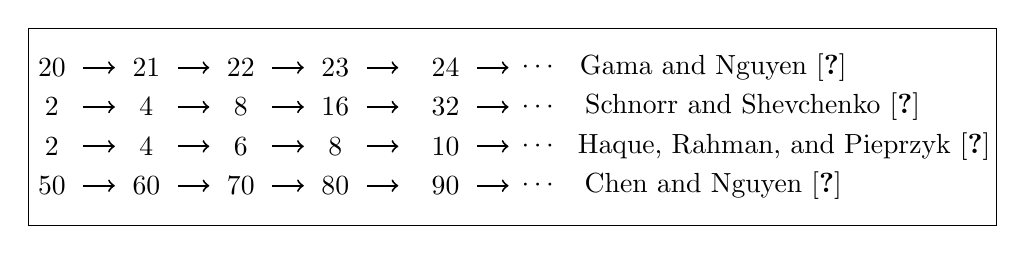
\begin{tikzpicture}
        %box drawing
        \draw[color=black] (-6.3,0) -- (6,0) -- (6,-2.5) -- (-6.3,-2.5) --  (-6.3,0);
        % horizental first
        \node at (-6,-.5) {20};
        \draw[->, line width=.25mm,  black] (-5.6,-.5)--(-5.2,-.5);
        \node at (-4.8,-.5) {21};
        \draw[->, line width=.25mm,  black] (-4.4,-.5)--(-4,-.5);
        \node at (-3.6,-.5) {22};
        \draw[->, line width=.25mm,  black] (-3.2,-.5)--(-2.8,-.5);
        \node at (-2.4,-.5) {23};
        \draw[->, line width=.25mm,  black] (-2,-.5)--(-1.6,-.5);
        \node at (-1,-.5) {24};
        \draw[->, line width=.25mm,  black] (-.6,-.5)--(-.2,-.5);
        \node at (.2,-.5) {$\cdots$};
        \node at (2.4,-.5) {\text{Gama and Nguyen} \cite{gama2008predicting}};
        % horizental Second
        \node at (-6,-1) {2};
        \draw[->, line width=.25mm,  black] (-5.6,-1)--(-5.2,-1);
        \node at (-4.8,-1) {4};
        \draw[->, line width=.25mm,  black] (-4.4,-1)--(-4,-1);
        \node at (-3.6,-1) {8};
        \draw[->, line width=.25mm,  black] (-3.2,-1)--(-2.8,-1);
        \node at (-2.4,-1) {16};
        \draw[->, line width=.25mm,  black] (-2,-1)--(-1.6,-1);
        \node at (-1,-1) {32};
        \draw[->, line width=.25mm,  black] (-.6,-1)--(-.2,-1);
        \node at (.2,-1) {$\cdots$};
        \node at (2.9,-1) {\text{Schnorr and Shevchenko} \cite{schnorr2012solving}};
        % horizental third
        \node at (-6,-1.5) {2};
        \draw[->, line width=.25mm,  black] (-5.6,-1.5)--(-5.2,-1.5);
        \node at (-4.8,-1.5) {4};
        \draw[->, line width=.25mm,  black] (-4.4,-1.5)--(-4,-1.5);
        \node at (-3.6,-1.5) {6};
        \draw[->, line width=.25mm,  black] (-3.2,-1.5)--(-2.8,-1.5);
        \node at (-2.4,-1.5) {8};
        \draw[->, line width=.25mm,  black] (-2,-1.5)--(-1.6,-1.5);
        \node at (-1,-1.5) {10};
        \draw[->, line width=.25mm,  black] (-.6,-1.5)--(-.2,-1.5);
        \node at (.2,-1.5) {$\cdots$};
        \node at (3.3,-1.5) {\text{Haque, Rahman, and Pieprzyk} \cite{haque2019analyzing}};
        % horizental fourth
        \node at (-6,-2) {50};
        \draw[->, line width=.25mm,  black] (-5.6,-2)--(-5.2,-2);
        \node at (-4.8,-2) {60};
        \draw[->, line width=.25mm,  black] (-4.4,-2)--(-4,-2);
        \node at (-3.6,-2) {70};
        \draw[->, line width=.25mm,  black] (-3.2,-2)--(-2.8,-2);
        \node at (-2.4,-2) {80};
        \draw[->, line width=.25mm,  black] (-2,-2)--(-1.6,-2);
        \node at (-1,-2) {90};
        \draw[->, line width=.25mm,  black] (-.6,-2)--(-.2,-2);
        \node at (.2,-2) {$\cdots$};
        \node at (2.4,-2) {\text{Chen and Nguyen} \cite{chen2011bkz}};
    \end{tikzpicture}
    \caption{Sequences of blocksizes that have been used after LLL-reduction in the previous literatures} %(Picture taken from \cite{laarhoven2012solving})}
    \label{fig:BKZ_Blocksize_increase}
\end{figure}
%--------------end lattice relation figure-----------------------



%Furthermore this work also proposed a simulator for predicting the length of the Gram-Schmidt basis obtained from the BKZ reduction and a model for estimating the computational cost of the proposed progressive BKZ by considering the efficient implementation of the local enumeration algorithm and the LLL algorithm. Later the work has been compare with that of other algorithms using instances from the Darmstadt SVP Challenge. Analytical experiments performed showed that the proposed algorithm is approximately $50$ times faster than that of the BKZ 2.0 when used for solving the SVP Challenge up to $160$ dimensions.


To decide the time to increase the block size $\beta$, progressive BKZ uses the Full Enumeration Cost (FEC)-- a concept derived from Gama-Nguyen-Regev's cost estimation [19] with a Gaussian heuristic radius and without pruning.
In previous works, the timing was often heuristic.
Thus, the authors in this work tried hard to develop a scientific formulation regarding time to increase the block size.

In progressive BKZ, the algorithm starts the BKZ algorithm with a relatively small blocksize $\beta_{start}$ and increases the blocksize to $\beta_{end}$.
To obtain a BKZ-$\beta$ reduced basis from a LLL reduced basis many blocksize strategies are considered as follows:
\begin{equation*}
    \beta_0^{goal}=LLL \xrightarrow{\beta_1^{alg}} \beta_1^{goal} \xrightarrow{\beta_2^{alg}} \beta_2^{goal} \xrightarrow{\beta_3^{alg}} \cdots \xrightarrow{\beta_D^{alg}}  \beta_D^{goal} (=\beta)
\end{equation*}

This sequence is also denoted by $\{(\beta_j^{alg},\beta_j^{goal})\}_{j=1,\cdots,D}$ and regarded it as the progressive BKZ.
This work employs full enumeration cost and Sim-FEC($n,\beta^{alg}$) to decide the block size increase condition.
Blocksize is increased when the condition  FEC($\pmb{B}$) $>$ Sim-FEC($n,\beta^{alg}$) fails and keeps on increasing until it reaches the condition FEC($\pmb{B}$) $<$ Sim-FEC($n,\beta^{goal}=\beta$), where $\beta^{alg}$ and $\beta^{goal}$ represents the intermediate blocksize and the target block size used in the progressive BKZ reduction.

The full enumeration cost for a basis $\pmb{B} = (\pmb{b}_1 , \cdots , \pmb{b}_n)$ of $n$-dimensional lattice $\Lambda$ is computed as
\begin{align*}
    \text{FEC}(\pmb{B}) & = \sum_{k=1}^n \frac{V_k(GH(\Lambda))}{\prod_{i=n-k+1}^n ||\pmb{b}_i^*||}
\end{align*}
where $||\pmb{b}_i^*||$ represents the GS-length.
Since $||\pmb{b}_1||$ is often larger than $\lambda_1(\Lambda)$, thus the search radius is set as $R_n=GH(\Lambda)$ to decrease the computational cost.
%Note that the FEC($\pmb{B}$) eventually decreases after performing several tours of the BKZ algorithm using the fixed blocksize $\beta$.


The simulator for an $n$-dimensional lattice depends only on the blocksize $\beta$ of the local block.
The simulated GS-length $(l_1 ,\cdots , l_n)$ is denoted by Sim-GS-lengths($n,\beta$).
A simulated Gaussian heuristic that is used in simulated GS-lengths$(l_1,\cdots,l_n)$ is defined as
\begin{align*}
    \text{Sim-GH}(l_1 , \cdots , l_n) & = V_n(1)^{-1/n} \prod_{j=1}^n l_j^{1/n}
\end{align*}
which is later used to compute the simulated value of the full enumeration cost as presented below
\begin{align*}
    \text{Sim-FEC}(l_1 , \cdots , l_n) & := \sum_{k=1}^n \frac{V_n(\text{Sim-GH}(l_1,\cdots,l_n))}{\prod_{i=n-k+1}^n l_i}
\end{align*}

%Furthermore the simulated enumeration cost Sim-ENUMCost$(l_1,\cdots,l_{\beta};\alpha,p)$ is defined by ENUMCost($B;\alpha,p$) for a lattice basis $\pmb{B}$ that has GS-lengths $||\pmb{b}^{*}_i||=l_i$ for $i \in [\beta]$.


Computation of simulated Gram-Schmidt lengths of $||b_i^*||$ using BKZ with blocksize $\beta$ performed in two steps.
In the first step, the initial value of $(l_1,\cdots,l_n)$ is computed.
This is done by setting $l_n=1$ and computing $l_i$ backwards using equation \ref{eq:l_i} below
\begin{equation}
    l_i = max \Big\{ \frac{\beta'}{\beta'+1} \alpha, \tau_{\beta'} \Big\} \cdot GH(l_i,\cdots,l_{i+\beta'-1}) \hspace{1.5em} where\ \beta'=min(\beta,n-i+1)
    \label{eq:l_i}
\end{equation}
Here $\alpha$ is the optimized radius parameter computed using equation \ref{eq:computing_r} above, and $\tau_{\beta'}$ is the coefficient of the modified Gaussian heuristic, where the modified Gaussian heuristic for $\tau_i$ is computed as
\begin{equation*}
    \tau_i= \frac{\lambda_1(\pi_{n-i+1}(\Lambda))}{GH(\pi_{n-i+1}(\Lambda))} = \frac{||\pmb{b}^{*}_{n-i+1}||} {V_i(1)^{-1/i} \cdot \prod_{j=n-i+1}^{n}||\pmb{b}^{*}_{j}||^{1/i}}
\end{equation*}


This is sufficient for the smaller block sizes viz., $\beta < 30$.
For simulating larger block sizes, we must modify the GS-lengths of the first and last indexes, and is done in the second step using the help of MINCost($\beta$), here MINCost($\beta$) represents the standard value of the enumeration cost of blocksize $\beta$.
For $i>n-\beta+1$, i.e., the situation where the blocksize is smaller than $\beta$ the modified GS-length is computed as
\begin{equation}
    l_i = max \Big\{ \frac{\beta'}{\beta'+1} \alpha_i, \tau_{\beta'} \Big\} \cdot GH(l_i,\cdots,l_{i+\beta'-1}) \hspace{1.5em} where\ \beta'=n-i+1
    \label{eq:l_i_small}
\end{equation}
Here $\alpha_i=(2/p_i)^{n-i+1}$.
Later for the first index's integer parameter, $b>0$ is used.
For $b=1,2,\cdots$ blocksize for index $i$ is computed as $\beta_i :=\beta+max\{(b-i+1),b-2(i-1)\}$ for $i\in \{1,\cdots,b\}$ using those blocksize GS-length is recomputed by using equation \ref{eq:l_i_small} from $i=\beta_i$ to $1$.
Further the value of Sim-ENUMCost($l_1 ,\cdots, l_{\beta+b}; \alpha, p$) is computed by selecting maximum $b$ that gives simulated enumeration cost smaller than $2 \cdot MINCost(\beta)$.

\begin{comment}
The expected number of BKZ tours in the progressive BKZ can be computed using equation \ref{eq:no_tours_bkz} below
\begin{equation}
    \#tours =(t-1)+ \frac{\text{Sim-FEC}(l_1',\cdots,l_n')-\text{Sim-FEC}(n,\beta)}{\text{Sim-FEC}(l_1',\cdots,l_n')-\text{Sim-FEC}(l_1,\cdots,l_n)}
    \label{eq:no_tours_bkz}
\end{equation}
Where the BKZ tour updates the pair $(l_i,l_{i+1})$ to $(l'_i,l'_{i+1})$ for $i=1,\cdots,n-1$ using the equation \ref{eq:l_i_update_1} and \ref{eq:l_i_update_2} below
\begin{align}
    l'_i     & = max \Big\{ \frac{\beta}{\beta+1}\alpha, \tau_{\beta} \Big\} \cdot GH(l_i,\cdots,l_{min(n,i+\beta-1)})
    \label{eq:l_i_update_1}                                                                                            \\
    l'_{i+1} & = l_{i+1} \cdot (l_i/l'_i)
    \label{eq:l_i_update_2}
\end{align}



Optimizing Blocksize Strategies: The optimal sequence that minimizes the total computing time can be given as
\begin{equation}
    \sum_{i=1}^D TimeBKZ(n,\beta_{i-1}^{goal} \xrightarrow{\beta_i^{alg}} \beta_i^{goal})
\end{equation}
\end{comment}


\begin{algorithm}[h!]
\KwData{Given a lattice basis $\pmb{B}$ of $n$-dimensions, Blocksize strategy $\{(\beta^{alg}_{j},\beta^{goal}_{j})\}_{j=1,\cdots,D}$}
\KwResult{A $\beta_D^{goal}$-reduced basis $\pmb{B}$}
$\pmb{B} \leftarrow LLL(\pmb{B})$; \\
\For{$j=1$ \KwTo $D$}
{
    \While{FEC($B$) $>$ Sim-FEC($n,\beta_j^{alg}$)}
    {
        \For{$i \leftarrow 1$ \KwTo $n-1$}
        {
            %Set $(\alpha,p)$ for local block $\pmb{B}_i$ of blocksize $\beta^{'}=min(\beta,n-i+1)$ \\
            %Preprocess the basis by the progressive BKZ; \\
            %Execute lattice enumeration with probability $p$ and radius $\alpha \cdot GH(\pmb{B}_i)$; \\

          %%%%%%%%%%%
          Compute the Gram-Schmidt lengths $||b^{*}_i||$ and coefficients $\mu_{ij}$ corresponding to the local block $B_i$ of blocksize $\beta'= min(\beta, n-i+1)$\\
          Set $(\alpha, p)$ for $B_i$; \\
          Set near optimized pruning coefficients $(R_1,\cdot, R_{\beta})$ for $(B_i,\alpha, p)$;
          Preprocess $B_i$ by the BKZ; \\
          \If {enumeration cost for $B_i$ computed using $(\alpha_p, R_1, \cdots , R_{\beta})$ is large}
            {
                optimize the bounding function;\\
            }
          $\{v_1, \cdots , v_h\} \leftarrow$ (lattice enumeration for $B_i$ using $(\alpha_p, R_1, \cdots , R_{\beta})$); \\
          Construct the degenerated basis \\
            $(\pmb{b}_1, \cdots , \pmb{b}_{i-1}, v_{i_1}, \cdots , v_{i_g}, b_i, \cdots , b_{i+\beta'-1})$\\
          Apply the LLL algorithm to the basis \\
            $(\pmb{b}_1, \cdots , \pmb{b}_{i-1}, \pmb{v}_{i_1}, \cdots , \pmb{v}_{i_g}, \pmb{b}_i, \cdots , \pmb{b}_{i+\beta'-1})$ \\
          and erase the zero vectors;\\
            \If {$||\pmb{v}|| < \alpha \cdot GH(\pmb{B}_i)$}
            {
                 update basis $\pmb{B}$ by $\pmb{v}$;
            }
        }
    }
}
\caption{Progressive BKZ algorithm}
\label{alg:Prog_BKZ_algo}
\end{algorithm}












\subsection{$\delta$ estimates}
In literature, few $\delta$ (root Hermite factor) estimates available for  BKZ with block size $\beta$.
These estimates can be used to predict the values of $\delta$ and/or to estimate the condition under which uSVP can be solved using lattice reduction.
We presented these estimates below:

\subsubsection{Chen estimate} Chen et al.
in \cite{chen2013reduction} estimated about $\delta$ obtained using BKZ with blocksize $\beta$ as
\begin{equation*}
    \delta(\beta)=\Big( \frac{\beta}{2\pi e} (\pi \beta)^{1/\beta} \Big) ^{\frac{1}{2(\beta-1)}}
\end{equation*}
For a large $\beta$, it is also estimated as equal to $\beta^{\frac{1}{2\beta}}$
\subsubsection{2008 estimate} Estimate provided by Gama and Nguyen in \cite{gama2008predicting} is also known as 2008 prediction.
The estimate claims that the shortest vector of a lattice can be recovered if
\begin{equation*}
    \gamma = \frac{\lambda_2}{\lambda_1} \geq \delta^n
\end{equation*}

\subsubsection{2016 estimate} Estimates provided by Alkim et al.
\cite{alkim2016post} is popularly known as the 2016 prediction.
Assuming that \textbf{Geometric Series Assumption} \cite{schnorr2003lattice} holds, the authors claimed that the norms of the Gram-Schmidt vectors after lattice reduction satisfy
\begin{equation*}
    ||\pmb{b}_i^*|| \approx \delta^{n-2i+2} \cdot Vol(\Lambda)^{1/n}
\end{equation*}
The reason behind the same is that if the projection of the unique shortest vector onto the space spanned by the last $\beta$ Gram-Schmidt vectors is shorter than $\pmb{b}_{n-\beta+1}^*$, then the SVP oracle in BKZ would be able to find it when called on the last block of size $\beta$.
Thus the success condition can be given as
\begin{equation*}
    \sqrt{\frac{\beta}{n}}\lambda_1 \leq ||\pmb{b}_{n-\beta+1}^*||
\end{equation*}



%Runtime estimates for the BKZ algorithm Dana paper as well

%Go through the new hope paper
%https://sites.math.washington.edu/~rothvoss/lecturenotes/IntOpt-and-Lattices.pdf
%https://www.youtube.com/watch?v=_WlMG81ifQs&ab_channel=TheIACR
%https://www.youtube.com/watch?v=7-RWAU8pBqI&ab_channel=TheIACR


%Runtime estimates for the BKZ algorithm Dana paper as well

%Go through the new hope paper
%https://sites.math.washington.edu/~rothvoss/lecturenotes/IntOpt-and-Lattices.pdf
%https://www.youtube.com/watch?v=_WlMG81ifQs&ab_channel=TheIACR
%https://www.youtube.com/watch?v=7-RWAU8pBqI&ab_channel=TheIACR



\subsubsection{Micciancio and Walter Prediction} In 2016, Micciancio et al.
\cite{micciancio2016practical} presented a technique to predict the output of the lattice basis reduction combining the best of both the world viz., BKZ \cite{schnorr1987hierarchy,schnorr1994lattice,chen2011bkz} and the Slide reduction algorithm introduced by Gama and Nguyen\cite{gama2008finding}.
BKZ performs well in practice; however, its asymptotic performance could be better.
Furthermore, its simple average case prediction is performed by a simulator which, in general, is based on some heuristics which need to be clarified if these hold.
Slide reduction, on the other hand, provides good simple average case prediction and asymptotic performance, but practical performance is believed to be not so great \cite{gama2008finding,gama2008predicting}.
It is claimed in \cite{gama2008finding} that BKZ with block size $k=20$ produces better-reduced bases than Slide reduction with block size $k=50$.



Thus performing an extensive experiment on several lattice reduction algorithms, both novel and from the literature, the authors claimed that to predict lattice reduction simulation is superfluous and can be replaced by a closed formula using weaker assumptions.
To reach this conclusion, the authors used a novel algorithm to solve the Shortest Vector Problem (SVP) in the dual without computing the dual basis, termed Self-Dual BKZ.
The new algorithm provides the same practical performance as that of the BKZ, asymptotic performance, and simple average case prediction as that of the Slide reduction.

\begin{comment}

\begin{algorithm}[H]
    \SetAlgoLined
    \LinesNumbered
    procedure DBKZ (\pmb{B}, k, SVP$_k$)\\
    \SetKwInOut{Input}{Input}
    \Input{A lattice basis $\pmb{B} \in \mathbb{Z}^{m\times n}$, a block size k, a SVP oracle in dimension k}
    \SetKwInOut{Output}{Output}
    \Output{A k-reduced basis $\pmb{B}'$}
    \SetKwProg{Function}{function}{}{end}
    \SetKwRepeat{Do}{do}{while}
    \While{progress is made}
    {
        Working fine
    }
    \KwRet {\pmb{B}}
    \caption{Self-Dual BKZ}
\end{algorithm}
\end{comment}


Implementation of this new SVP solving technique can be easily added to the existing primal implementation with obtained efficiency the same as that of the primal algorithm.

 %Lattices basics and lattice reduction techniques


% !TeX root = ../sameplaper.tex
% !TeX spellcheck = en_US

\chapter{Lattice Attacks}
\setcounter{section}{0}


\section{Known attacks and their computational complexity}
In this section, we will discuss possible attacks to break above mentioned hard problems and use them to suggest concrete parameters for practical applications.

This section reviews the algorithms for solving the LWE, AGCD, and NTRU problems and tries to suggest concrete parameter choices based on different works available in the literature \cite{}. The hardness of these problems has been studied in terms of only asymptotic notations in much of the literature. Asymptotic notations usually give a good overview of the general behavior of an algorithm. However, simultaneously, it might result in weaker parameter settings as it may hide logarithmic and constant factors in the exponent. Therefore, it has to be taken care of when determining the secure parameters while designing a cryptosystem.

While discussing the hardness of LWE and RLWE assumptions, we want to make sure that RLWE is instantiated with rings that are $2$-power or prime cyclotomic rings, and we do not currently know better attacks on RLWE than that of LWE problem \cite{}. The NTRU problem can also be considered as the homogeneous version of the RLWE problem. For the NTRU problem, a subfield attack has been proposed in the literature to break the homomorphic encryption schemes based on it \cite{albrecht2016subfield}. However, as of now, there is no indication that these attacks can be translated to the RLWE problem settings \cite{albrecht2017dual}. No known attack algorithms solve the RLWE problem faster than the LWE problem for the parameter choices typically considered in the fully homomorphic encryption settings. Thus, we discuss estimates and attacks for the LWE problem with some parameters used in FHE. However, we will also discuss some security-related issues varying the ring choice.

Among the main proposed approaches for solving LWE instances includes the following
\begin{enumerate}
    \item Attack using Lattice algorithms
    \item Attack using Algebraic algorithms
    \item Attack using Combinatorial algorithms
    \item Attack using Side-channel Information
    \item Attack on Small LWE variant


\end{enumerate}
We will briefly discuss each of the above algorithms one by one, starting with the lattice algorithms.




\subsection{Attack using Lattice algorithms}
The lattice algorithm can be further categorized into three categories based on their approach to solving the LWE problem.
\begin{enumerate}
    \item Primal attack by solving Bounded Distance Decoding (BDD) problem
    \item Primal attack by solving unique Shortest Vector (uSVP) Problem
    \item Dual attack by solving Short Integer Solution (SIS) problem
\end{enumerate}
Here we consider all possible approaches for solving LWE, including the algorithms that may require many samples ($m$). We assume that the attacker has access to an unlimited number of samples. Thus we parameterize an LWE instance by $n,\alpha$, and $q$.

However, in practical scenarios allowing an unlimited number of samples may not always be feasible since there are scenarios in which an attacker attempting to solve LWE would only have access to a limited number of samples. Hence it can be argued that allowing unlimited samples, and thus assuming the attacker is more powerful, may lead to overly conservative security estimates. This issue is addressed by Bindel et al. \cite{bindel2019estimation} by implementing an extension to the LWE estimator \cite{albrechtestimator} that enables the user to specify a limit on the number of samples, in addition to number of samples $m$ the usual parameters $n, \alpha$ and $q$, and then obtain an estimate of the hardness of the LWE instance in this case.

Below we have presented each of the LWE-solving techniques briefly.



\subsubsection{Primal attack by solving Bounded Distance Decoding (BDD)\label{Primal_BDD}}
Lindner and Peikert present this attack \cite{lindner2011better} to use to solve the Search-LWE problem. LWE problem can be viewed as an average-case `bounded-distance decoding' problem on a certain family of lattices. Given an LWE problem with $(\textbf{A},\textbf{b})$, where $\textbf{A} \in \mathbb{Z}^{n\times m}_q$, the corresponding lattice can be defined as

\begin{align*}
    \Lambda(\textbf{A}^t) & = \{ \textbf{z} \in \mathbb{Z}^m : \exists \textbf{s} \in \mathbb{Z}^n_q \ \text{such  that } \textbf{z}=\textbf{A}^t\textbf{s}\ mod\ q \}
\end{align*}

Here the component $\textbf{b}=\textbf{As}+\textbf{e}$ of the LWE input may be seen as a perturbed lattice point in $\Lambda(\textbf{A}^t)$. Perturbed by a small error $\textbf{e}$ sampled from Gaussian distribution with mean zero and standard deviation $\sigma$. In this case, our solution to the BDD problem is the lattice point $\textbf{z}$. Given $(\textbf{A},\textbf{z})$, linear algebra can be used to recover the secret vector $\textbf{s}$ viz. to solve the search LWE problem.

To recover the lattice vector $\textbf{z}$, a basis matrix $\textbf{B}$ is constructed, which is latter reduced using lattice reduction algorithms viz. LLL, BKZ, or its enhanced version BKZ2.0 with a  block size $\beta$. The reduced basis matrix is latter fed to the modified recursive Nearest Plane algorithm of Babai \cite{babai1986lovasz} along with the target vector $\textbf{b}$. The algorithm should output a lattice vector $\textbf{v} \in \mathcal{L}(\textbf{B})$, that is relatively close to the target vector $\textbf{t}$. The output lattice vector $\textbf{v}$, for the input target vector $\textbf{t}=\textbf{v}+\textbf{e}$ is correctly provided $\textbf{e}$  happens to lie in the fundamental parallelepiped of the Gram-Schmidt orthogonalization (GSO) of $\textbf{B}$ viz. in $\mathcal{P}_{1/2}(\tilde{\textbf{B}})$.

Lindner and Peikert in \cite{lindner2011better} noted that in the reduced basis $\textbf{B}$, the fundamental parallelepiped is long and skinny, concurrently by the Geometric Series Assumption (GSA) due to Schnorr, the GSO of a BKZ-reduced basis decay geometrically making the probability that the Gaussian error vector $\textbf{e}$ falls in the corresponding fundamental parallelepiped very low. They addressed this issue by recursing the algorithm for $d_i \geq 1$ distinct planes at each recursion level. The affect of multiple recursion makes the parallelepiped $\textbf{P}_{1/2}(\tilde{\textbf{B}})$ wider by the same multiple $d_i$. This can be seen as a form of pruned CVP enumeration in the work of Liu et al. \cite{liu2013solving}. The increased success percent comes at the cost of increased runtime of the Nearest Planes algorithm, as it mainly depends on the number of points enumerated, which in this case, is the product of the scaling factors. However, the scaling factors alone don't determine the success probability; it also depends upon the quality of the reduced basis used. Thus to maximize the success probability, a proper scaling factor needs to be used, which is determined (predicted) based on the quality of the reduced basis used. There is no closed formula to predict the proper scaling factor; thus, the estimator uses a simple greedy algorithm to find it. However, this is not known to be optimal. Generally, the scaling factor and basis quality are decided based on the success percent required and the affordable runtime. More detail about the attack can be obtained in Lindner and Peikert \cite{lindner2011better}.



\subsubsection{Primal attack by solving unique Shortest Vector Problem (uSVP)\label{Primal_uSVP}}
Another primal attack to solve the LWE problem is to solve the unique shortest vector problem. Though in the literature, it has been shown that BDD and uSVP are polynomial-time equivalent for small approximation factors up to $\sqrt{n/\log{n}}$ \cite{lyubashevsky2009bounded}. However, the complexity study of the same has been recently performed by Albrecht et al. \cite{albrecht2014efficacy} presenting the technique for solving LWE problems using uSVP.

Assuming the secret has a small norm, the LWE problem is initially converted into a BDD problem, as mentioned in section \ref{Primal_BDD}. Later the BDD problem is transformed into an instance of the uSVP problem using Kannan's \cite{kannan1987minkowski} embedding technique, as shown below.

\begin{equation*}
    \textbf{B}_1 =\begin{pmatrix}
        \pmb{B}_0 & \hspace{1em} \pmb{b}' \\
        0         & \hspace{1em}  t
    \end{pmatrix} =
    \begin{pmatrix}
        \pmb{I}_n &  &  & \pmb{0}    & 0       \\
        \pmb{A}   &  &  & q\pmb{I}_m & \pmb{b} \\
        0         &  &  & 0          & t
    \end{pmatrix}
\end{equation*}
where $\pmb{b}'=(\pmb{0}||\pmb{b})$, $||$ represents the concatenation operation. The lattice generated by the columns of $\pmb{B}_1$ contains the unique shortest vector, as shown below

\begin{equation*}
    \pmb{B}_1  \begin{pmatrix}
        \hspace{1em} \pmb{s} \\
        \hspace{1em} \pmb{c} \\
        -1
    \end{pmatrix} =
    \begin{pmatrix}
        \pmb{B}_0
        \begin{pmatrix}
            \pmb{s} \\
            \pmb{c} \\
        \end{pmatrix}+
        \begin{pmatrix}
            \hspace{1em} \pmb{0} \\
            \pmb{-b}             \\
        \end{pmatrix}
        \\
        -t
    \end{pmatrix} =
    \begin{pmatrix}
        \hspace{1em} \pmb{s} \\
        -\pmb{e}             \\
        -t
    \end{pmatrix}
\end{equation*}


This attack tries to directly find the secret vector $\textbf{s}$ from the given LWE samples $(\textbf{A},\textbf{b})$ using the Kannan's embedding technique \cite{kannan1987minkowski} with embedding factor $t$. % (in practice, usually $t=1$).
Here the search version of the LWE problem is solved by finding a unique shortest vector generated by the following $q$-ary lattice.
\begin{equation*}
    \textbf{B} =\begin{pmatrix}
        A^T & 0 \\
        c^T & t
    \end{pmatrix}
\end{equation*}
Since
\begin{equation*}
    (\textbf{s}|-1)\cdot \textbf{B}=(\textbf{e} | -t) \ mod\ q
\end{equation*}

The basis construction for the same can be performed by reducing matrix $\textbf{A}^T \in \mathbb{Z}_q^{n\times m}$, $(m>n)$ into row echelon form to obtain $[\textbf{I}_{n} | \textbf{A}']$ followed by appending $[\textbf{0}|q\textbf{I}_{m-n}]$ (to handle the modular reduction) and $[\textbf{c}^T|t]$, to obtain a $(m+1)$-dimensional $q$-array lattice as

\begin{equation*}
    \textbf{B} =\begin{pmatrix}
        \textbf{I}_{n}     \ \  & \textbf{A}'                   \ \  & 0 \\
        \textbf{0}         \ \  & q\textbf{I}_{m-n}             \ \  & 0 \\
        \textbf{c}^T       \ \  & \ \                                & t \\
    \end{pmatrix}
\end{equation*}

Here $t=dist(\textbf{c},\textbf{L(A)})$ is the embedding factor. Lyubashevsky and Micciancio \cite{lyubashevsky2009bounded} showed that if $t < \frac{\lambda_1{(L(A))}}{2\cdot \gamma}$, then $\textbf{L(B)}$ contains a $\gamma$-unique shortest vector as $c'=(e,-t)$. If we can recover this vector, the problem is solved.

The problem can be solved by reducing it to $k$-\textit{Hermite Shortest Vector Problem} ($k$-HSVP). It has been shown by Lov\'{a}sz \cite{lovasz1986algorithmic} that any algorithm that can solve $k$-HSVP problem can be used linearly many times to solve approximate SVP with approximation factor $k^2$. A solution to $k^2$-approximate SVP would be a vector $v$ such that $||v||_2 \leq k^2\cdot \lambda_1(L)$. In a lattice with $k^2$-uSVP structure, any vector $w$ that is not the shortest vector and is independent of the shortest vector satisfies $||w||_2 \geq \lambda_2(L) > k^2\cdot \lambda_1(L)$. Thus we must have $\textbf{v}$, a multiple of the shortest vector; hence we have solved the problem we were trying to solve for $\gamma=k^2$. This bound has been improved by Ling et al. \cite{luzzi2013decoding} showing that, for a $N$ dimensional lattice, if $k>\sqrt{N}$ then any algorithm that can solve the $k$-HSVP can solve the $\gamma$-uSVP for $\gamma \approx \sqrt{N}_k$.

When the secret vector $s$ is short, a second established embedding technique reduces the LWE problem to the uSVP problem \cite{bai2014lattice,albrecht2017revisiting}. It can be seen that the vector $(\nu \textbf{s}| \textbf{e}|1)$, for some $\nu \ne 0$, is contained in the following lattice
\begin{equation*}
    \Lambda= \Big\{\textbf{x} \in (\nu \mathbb{Z})^{n} \times \mathbb{Z}^{m+1}\ |\ \textbf{x}\cdot \Big(\frac{1}{\nu} \textbf{A}\ |\ \textbf{I}_m \ |\ -\textbf{c} \Big)^{T} \equiv 0 \ \text{mod} \ q \Big\}
\end{equation*}
Here, $\nu$ is the balancing factor that balances the size of the secret and the noise. The square basis matrix $\textbf{M}$ of $(n+m+1)$-dimension for the above lattice $\Lambda$ can be constructed as

\begin{equation*}
    \textbf{M} =\begin{pmatrix}
        \nu \textbf{I}_n & -\textbf{A}^T & \textbf{0} \\
        \textbf{0}       & q\textbf{I}_m & \textbf{0} \\
        \textbf{0}       & \textbf{c}    & 1          \\
    \end{pmatrix}
\end{equation*}

Here the basis matrix $\textbf{M}$ is full rank, det($\textbf{M}$)=Vol($\Lambda$) and the integer span of $\textbf{M} \subseteq \Lambda$, as

\begin{equation*}
    \begin{pmatrix}
        \nu \textbf{I}_n & -\textbf{A}^T & \textbf{0} \\
        \textbf{0}       & q\textbf{I}_m & \textbf{0} \\
        \textbf{0}       & \textbf{c}    & 1          \\
    \end{pmatrix}
    \Big(\frac{1}{\nu} \textbf{A}\ |\ \textbf{I}_m \ |\ -\textbf{c} \Big)^{T} = \big( \textbf{A}-\textbf{A}\ |\ q\textbf{I}_m\ |\ \textbf{c}-\textbf{c}\big)^T \equiv \textbf{0} \ \text{mod} \ q
\end{equation*}

Note that $(\textbf{s}|*|1)\cdot \textbf{M}=(\nu\textbf{s}|\textbf{e}|1)$ for a suitable value of $*$. If the secret $\textbf{s}$ is small or sparse, as is used in homomorphic encryption libraries, choosing $\nu=1$ results in unbalanced vector $(\textbf{s}|\textbf{e}|1)$, i.e., $\frac{||s||}{\sqrt{n}} \ll \frac{||e||}{\sqrt{m}} \approx \sigma$, where $\sigma$ is the standard deviation of the LWE error distribution. Thus an appropriate value of $\nu$ is chosen to re-balance. Re-balancing not only preserves $(\textbf{s}|\textbf{e}|1)$ as the unique shortest vector in the lattice, it also increases the volume of the lattice being reduced; as a result, the reduced number of block size is required for the lattice reduction.

For example, when the secret is sampled from the ternary distribution $||\nu\textbf{s}||^2 \approx \frac{2}{3}\nu^2n$. By choosing $\nu=\sqrt{\frac{3}{2}}\sigma$ it results to $||\nu\textbf{s}||\approx \sigma \sqrt{n}$ and $(\textbf{s}|\textbf{e}|1) \approx \sigma\cdot\sqrt{n+m}$. Similarly, if $w<n$, entries of $\textbf{s}$ are non-zero from $\{1,-1\}$, we get $||\nu\textbf{s}||^2 =w \nu^2$, thus by setting $\nu=\sigma\sqrt{\frac{n}{w}}$ we obtain a vector $\nu\textbf{s}=\sigma\sqrt{n}$.


\subsubsection{Dual attack by solving Short Integer Solution (SIS)}
\label{Text:Deal_attack}
The dual strategy solves the Decisional-LWE problem by solving the Shortest Integer Solution (SIS) problem. Here the goal is to distinguish the LWE sample from randomly sampled samples. This is done by finding a short vector $\textbf{v}$ in the following dual lattice generated by $\textbf{A}$.
\begin{equation*}
    \Lambda(\textbf{A}^t)=\{\textbf{w} \in \mathbb{Z}_q^m\ | \ \textbf{wA} \equiv 0 \ \text{mod}\ q\}
\end{equation*}
Finding a short vector from the above lattice is equivalent to solving the Short Integer Solution problem. Equivalently, the points of $\Lambda(\textbf{A}^t)$ may be partitioned into hyperplanes orthogonal to $\textbf{v}$, successively separated by distance $\frac{q}{||\textbf{v}||}$.

Vector $\textbf{v}$ computed above helps us to distinguish LWE samples from the uniform samples as the inner product of
\begin{equation*}
    <\textbf{v},\textbf{b}>\ = <\textbf{v},\textbf{As}+\textbf{e}>\ = <\textbf{v},\textbf{As}> +<\textbf{v},\textbf{e}>\ \equiv_q <\textbf{v},\textbf{e}>
\end{equation*}
This approximately follows a Gaussian distribution over $\mathbb{Z}$ modulo $q$, assuming not too many of the components of $\textbf{v}$ are too large. In general $<\textbf{v},\textbf{b}>$ is uniform if $\textbf{b}$ is uniform over $\mathbb{Z}_q$, but when it is LWE sample it result into $<\textbf{v},\textbf{e}>$, which is small as both $\textbf{v}$ and $\textbf{e}$ are small. The advantage $\epsilon$ of distinguishing an LWE sample from that of the uniformly random sample can be given from the following result.
\begin{lemma} \cite{lindner2011better}
    The advantage of distinguishing a LWE sample parameterized by $n,\alpha$ and $q$ from that of random sample can be given as $\text{exp}(-\pi\cdot(||\textbf{v}||\cdot \alpha)^2)$, where $||\textbf{v}||$ is the length of the vector $\textbf{v}$ computed in the dual lattice $\Lambda(\textbf{A}^t)=\{\textbf{w} \in \mathbb{Z}_q^m\ | \ \textbf{wA} \equiv 0 \ \text{mod}\ q\}$ and $\alpha$ is the error rate.
\end{lemma}

For example, when the length of the vector $||\textbf{v}||=\frac{4}{\alpha}$, the distinguishing advantage is about $2^{-72}$. However, to distinguish with better advantage, one needs to have $||\textbf{v}|| \leq \frac{1}{2\cdot\alpha}$ or so, but this requires more effort. Also, it is clear from above that for an advantage $\epsilon$, the length of the vector $\textbf{v}$ needs to be  $||\textbf{v}||=\frac{1}{\alpha} \cdot \sqrt{\frac{ln(\frac{1}{\epsilon})}{\pi}}$.

There is a direct relationship between success probability and time to obtain the short vectors. Usually, depending upon the algorithm used to obtain vector $\textbf{v}$, it might be advantageous to accept longer vectors than short vectors. Accepting long vectors may result in a decreased distinguishing advantage, but this can be compensated using the Chernoff bound \cite{chernoff1952measure} i.e., running the algorithm about $\frac{1}{\epsilon^2}$ times, which results in success probability nearly close to $1$. In fact, this might be the faster alternative than running the algorithm to obtain short vectors, which requires more time to get those vectors and, thus, more running time.

In literature, it has been claimed that dual attacks are rarely better than primal ones \cite{albrecht2018estimate}.





\subsection{Attack using Algebraic algorithms: Arora-Ge algorithm}
In \cite{arora2011new}, Arora-Ge proposed the first algebraic algorithms to solve the LWE problem. The technique reduces the LWE problem to find the common root of a multivariate system of high-degree, error-free polynomials. The technique can solve the LWE problem in $2^{\tilde{O}(n^{2\epsilon})}$ operations, making it sub-exponential when $\epsilon<\frac{1}{2}$.

Given LWE sample $(\textbf{a}, \textbf{c}) \in \mathbb{Z}^{n+1}_q \times \mathbb{Z}_q$, write $f = c - \sum_{i=1}^{n} a_i\cdot x_i$, with $x_i$ representing the variables. Assuming that the error $\textbf{e}$ falls in the interval $\{-T, \cdots , T\}$, then the polynomial $F =f \cdot \Pi_{i=1}^T(f + i) \cdot (f - i)$ of degree $2T + 1$ evaluates to zero when $\textbf{x} = \textbf{s}$. If $T < \lfloor \frac{q}{2} \rfloor$, then $F = 0$ is a constraint on the possible values for the secret vector $\textbf{s}$. Thus collecting many such equations and solving the resulting multivariate high-degree system of equations recovers the secret key $\textbf{s}$. Arora-Ge used the linearisation method to solve these systems of equations. The number of samples needed for this technique to work is $\textbf{O}(n^{2T+1})$. Considering more samples increases the probability of noise falling outside the chosen interval of $\{-T, \cdots, T\}$, invalidating the constraint $F=0$. Thus, as the number of samples grows, it is required to have more value for $T$ so that the polynomials system remains error-free. This results in a further increase in number of samples. Arora-Ge has thoroughly analyzed and studied the trade-off to solve the LWE problem in \cite{arora2011new}. Albrecht et al. \cite{albrecht2014algebraic} performed a further study of the Arora-Ge algorithm and mentioned the following complexity result.

\begin{theorem}
    \cite{albrecht2014algebraic}
    Given LWE sample with parameters $n,q,\sigma=\alpha q/ \sqrt{2\pi}$, $2\leq \omega <3$ be the linear algebra constant and $D_{AG}=8\sigma^2\log{n}+1$.
    If $D_{AG}\in o(n)$ then Arora-Ge algorithm solves the computational LWE problem in time
    \begin{equation*}
        O\Big(2^{\omega\cdot D_{AG}\log{\frac{n}{D_{AG}}}}\cdot \sigma q \log{q} \Big) =O\Big(2^{8\omega\sigma^2\log{n}(\log{n}-\log{(8\sigma^2\log{n})})}\Big)
    \end{equation*}
    and memory
    \begin{equation*}
        O\Big(2^{2\cdot D_{AG}\log{\frac{n}{D_{AG}}}}\cdot \sigma q \log{q} \Big) =O\Big(2^{16\sigma^2\log{n}(\log{n}-\log{(8\sigma^2\log{n})})}\Big)
    \end{equation*}
    If $n\in o(D_{AG})$ then Arora-Ge algorithm solves the computational LWE problem in time
    \begin{equation*}
        O\Big(2^{\omega n \log{\frac{D_{AG}}{n}}}\cdot \sigma q \log{q} \Big) =O\Big(2^{\omega n\log{(8\sigma^2\log{n})}-\omega n \log{n}}\Big)
    \end{equation*}
    and memory
    \begin{equation*}
        O\Big(2^{2n \log{\frac{D_{AG}}{n}}\cdot \sigma q \log{q}} \Big) =O\Big(2^{2n\log{(8\sigma^2\log{n})}-2n\log{n}}\Big)
    \end{equation*}
\end{theorem}

Albrecht in \cite{albrecht2014algebraic} further showed that using Gr\"{o}bner basis Arora-Ge algorithm can be improved. Arora-Ge used the linearisation method to solve LWE using $O(n^d)$ LWE samples. This can be reduced using Gr\"{o}bner basis but at the cost of a more expensive solving step. However, this approach requires an assumption that random systems behave like semi-regular sequences; justification of the same can be obtained in \cite{albrecht2014algebraic}. In particular, when $\alpha q=\sqrt{n}$, following result is obtained

\begin{theorem}
    For a given LWE sample $(\textbf{a}_i, \textbf{c}_i) \in \mathbb{Z}^{n+1}_q \times \mathbb{Z}_q$ for $i\geq1$, $\alpha q =\sqrt{n}$ and $\omega$, a linear algebra constant. There is a heuristic algorithm to recover the secret in time complexity $O(2^{2.35\omega n+1.13n})$, memory complexity $O(2^{5.85n})$ and sample complexity $m=exp(\frac{\pi}{4}\cdot n)$
\end{theorem}



\subsection{Attack using Combinatorial algorithms: BKW algorithm}
BKW algorithm, named using the first letters of its inventors Blum-Kalai-Wasserman \cite{blum2003noise}, was initially proposed to solve the Learning Parity with Noise (LPN) problem. It is a combinatorial algorithm to solve the LPN problem; however, it can also be easily adapted to solve the LWE problem. Recently, further investigation of the algorithm has been performed by Albrecht et al. in \cite{albrecht2014algebraic} and suggested some complexity measures, as presented in the later part of the section.

The algorithm works in two phases, the reduction phase and the solving phase. In the reduction phase, a series of operations are performed, known as BKW steps. These steps iteratively reduce the dimension of the problem, however, at the cost of increasing noise level. At the end of the reduction phase, we get a transformed problem with a much smaller dimension but higher noise. The transformed new problem is later solved efficiently by distinguishing in the solving phase.

BKW algorithm is parameterized by $a$ and positional value, say $b=\frac{n}{a}$, in the LWE sample vectors. Two samples are included in the same category if and only if $b$ positional values get canceled when added or subtracted. For example, assuming we have two samples $\textbf{a}_1$ and $\textbf{a}_2$ within the same category. Now, adding/subtracting these two sample results into
\begin{equation*}
    \textbf{a}_{12}=[\underbrace{0,0, \cdots 0}_\text{b variables},*, *,\cdots, *]
\end{equation*}
The resulting final sample we get after addition/subtraction is the sample $\textbf{a}_{12}$. The noise of the variable increases up to $e_{12}=e_{2}+e_{2}$, with variances $2\sigma^2$, where $\sigma^2$ is the variance of the original noise. Thus, by performing the above step in each category, we have successfully reduced the number of variables by $b$  but at the cost of increasing noise variance by $2\sigma^2$. Repeating the above step for a say $t$ number of times, we can successfully reduce the number of variables or the problem's dimensionality by $(n-tb)$ with the cost of increasing noise variance by $2^t\cdot \sigma^2$. The following results have been observed by Albrecht et al. in \cite{albrecht2014algebraic}.

\begin{theorem} \cite{albrecht2014algebraic,c54b603f579b48a08b698bde47b71455}
    Let $(\textbf{a}_i , c_i)$ be a LWE sample or a uniform distribution on $\mathbb{Z}_q^n \times \mathbb{Z}_q$ , $0 < b \leq n$ and $a =\lceil\frac{n}{b}\rceil$, say $0<\epsilon<1$ be the targeted success rate. Then the expected cost of the BKW algorithm to distinguish LWE sample from a random sample with success probability $\epsilon$ is
    \begin{equation*}
        \Big(\frac{q^b-1}{2}\Big) \cdot \Big(\frac{a(a-1)}{2}\cdot(n+1)-\frac{ba(a-1)}{4}-\frac{b}{6} \Big((a-1)^3+\frac{3}{2}(a-1)^2+\frac{1}{2}(a-1)\Big)\Big)
    \end{equation*}
    addition/subtraction are performed in $\mathbb{Z}_q$ to obtain the elimination tables,
    \begin{equation*}
        \frac{1}{exp(-\pi\alpha^2 2^{a})^2} \cdot\Big(\frac{a}{2}\cdot(n+2)\Big)
    \end{equation*}
    addition/subtraction are performed in $\mathbb{Z}_q$ to obtain new samples. Furthermore,
    \begin{equation*}
        a\cdot \Big\lceil \frac{q^b}{2} \Big\rceil + \frac{1}{exp(-\pi \alpha^2 2^a)^2}
    \end{equation*}
    calls are performed to the LWE sampler and storage for
    \begin{equation*}
        \Big( \frac{q^b}{2} \cdot a \cdot \Big( n+1-b\cdot \frac{a-1}{2} \Big)
    \end{equation*}
    elements in $\mathbb{Z}_q$ are needed
\end{theorem}




\begin{theorem} \cite{albrecht2014algebraic,c54b603f579b48a08b698bde47b71455}
    Given LWE samples $(\textbf{a}_i,c_i)$ from LWE sampler and setting $a=\lfloor \log_2{(1/(2\alpha)^2} \rceil$, $b=\frac{n}{a}$, and $q$, a prime number. Let $d$ be a small constant $0<d<\log_2{(n)}$. Assuming $\alpha$ as such that $q^b=q^{n/a}=q^{n/\lfloor \log_2(1/(2\alpha)^2) \rceil}$ is superpolynomial in $n$. Provided the above parameters, the cost of solving the BKW algorithm to solve Search-LWE is
    \begin{equation*}
        \Big(\frac{q^b-1}{2}\Big) \cdot \Big(\frac{a(a-1)}{2}\cdot(n+1)\Big) + \Big\lceil \frac{q^b}{2} \Big \rceil \cdot \Big(\Big\lceil \frac{n}{d} \Big\rceil +1 \Big)\cdot d \cdot a + poly(n) \approx (a^2n)\cdot \frac{q^b}{2}
    \end{equation*}
    operations in $\mathbb{Z}_q$. Furthermore,
    \begin{equation*}
        a\cdot \Big\lceil\frac{q^b}{2} \Big\rceil +poly(n)
    \end{equation*}
    calls to the LWE sampler and storage of
    \begin{equation*}
        \Big( a \cdot \Big \lceil \frac{q^b}{2} \Big \rceil \cdot n \Big)
    \end{equation*}
    $\mathbb{Z}_q$ elements are needed
\end{theorem}

Many improvements to the plain BKW steps have been proposed in the literature, viz. lazy modulus switching by Albrecht et al. in \cite{albrecht2014lazy}, which is further developed by Kirchner et al. in \cite{kirchner2015improved}. In \cite{guo2015coded}, Guo et al. introduced Coded-BKW, the idea is to map the vectors to the lattice codeword that is nearest in Euclidean norm, such that the vectors that are mapped to the same Codeword get canceled. Using coded-BKW, noise introduced in the process can be controlled so that it is not more than the noise that would have been introduced with a standard BKW procedure. Later, BKW with sieving is introduced by Guo et al. in \cite{guo2017coded} and is improved in \cite{guo2019asymptotics,maartensson2019asymptotic}.

It has been observed by Albrecht et al. in \cite{albrecht2017dual} that the BKW-type algorithm can be seen as a general framework where firstly, a smaller dimensional LWE instance is created using iteration of some quantization technique, then the obtained smaller dimensional instance is solved using any preferred method.


Attack using Side-channel Information




\subsection{Attack using Side Information}
Based on how a computer protocol or algorithm is implemented, it can leak some information to the environment. These pieces of information are not because of the flaws in the protocol design or algorithm itself but potentially devastating mistakes or oversights in the implementation. A few sources of side-channel leakage include cold boot, timing information, power consumption, electromagnetic leaks, flush gauss and reload of cache, differential fault, existential forgery, practical fault, sound information, etc., which could be exploited to facilitate the side-channel attacks. However, when these pieces of information are used standalone to construct the secret information, new techniques, and algorithms are required to be developed for each of these settings. Moreover, when these techniques are used ad-hoc, we need to find a way to take advantage of decades worth of research and help optimize the standard lattice attacks. Moreover, most of the side-channel attacks from prior work consider substantial amounts of information leakage and show that it leads to feasible recovery of the entire key. In contrast, it might be interesting if more precise trade-offs in terms of information leakage versus the concrete security of the scheme could be obtained.

To answer these questions, Dana et al. in \cite{dachman2020lwe} created a toolkit to integrate side channel information in the form of ``hints", about the secret and/or error, into the uSVP instance, which is later solved using a lattice-reduction algorithm. They have observed that integrating side-channel information into the lattice reduction attacks results in a less secure scheme. Their attack technique generalizes the so-called primal lattice reduction attack and allows the progressive integration of hints before running a final lattice reduction step. In short, integrating hints include sparsifying the lattice, projecting onto and intersecting with hyperplanes, and/or altering the distribution of the secret vector.

Their technique primarily generalizes the Bounded Distance Decoding problem (BDD) to a Distorted version (DBDD). An instance of DBDD consists of three parts: lattice $\pmb{\Lambda}$, mean vector $\pmb{\mu}$, and covariance matrix $\pmb{\Sigma}$. Here the lattice $\pmb{\Lambda}$ represents the lattice obtained by Kannan's embedding- a way to construct a lattice where the LWE secret/error is the shortest non-zero vector. The side information can be used to sparsify or reduce the dimension of the original lattice. The remaining part, viz. $(\pmb{\mu,\Sigma})$ corresponds to the mean vector and covariance matrix, representing the distributional information about the LWE secret/error. Here $(\pmb{\mu,\Sigma})$ represents that the secret/error is drawn from a distribution with known mean/covariance determined by the specifications of the cryptosystem. Subsequently, given the side information, it captures the conditional distribution on the secret/error in cases where it remains well approximated by a Gaussian. Thus, certain types of information on the structure or on the distribution of the secret can be integrated into a DBDD instance, starting with the original instance and then modifying $\pmb{\Lambda}$, and/or $(\pmb{\mu, \Sigma})$ appropriately.

A DBDD instance is later converted into a uSVP instance by performing two steps, viz. first homogenization—centering the ellipsoid at the origin and second isotropization—applying a linear transformation that simultaneously transforms the ellipsoid into a ball and transforms the lattice into a different lattice with higher volume. Finally, the resulting uSVP instance is fed into the lattice reduction algorithm to obtain the shortest non-zero vector in the transformed lattice. The recovered short non-zero vector is later used to retrieve the LWE secret/error. The major steps mentioned above can be pictorially presented in figure \ref{fig:Lwe_with_side_information}.


% (refer defination \ref{def:DBDD}), which allows to account for the potentially non-spherical covariance of the secret vector that needs to be found.

% \begin{definition} \cite{dachman2020lwe}
%     (Distorted Bounded Distance Decoding problem) Let $\bold{\Lambda} \subset \mathbb{R}^d$ and $\bold{\Sigma} \in \mathbb{R}^{d\times d}$ represents the lattice and symmetric matrix respectively and $\pmb{\mu} \in Span(\bold{\Lambda}) \subset \mathbb{R}^d$ such that
%     \begin{equation*}
%          Span(\bold{\Sigma}) \subsetneq Span(\bold{\Sigma} + \pmb{\mu}^T \cdot \pmb{\mu}) = Span(\bold{\Lambda})
%     \end{equation*}
%     The Distorted Bounded Distance Decoding problem DBDD$_{\pmb{\Lambda,\mu,\Sigma}}$ can be defined as follows:

% \textbf{Given} $\pmb{\mu}, \pmb{\Sigma}$ and a basis of $\bold{\Lambda}$.

% \textbf{Find} the unique vector $\bold{x} \in \bold{\Lambda}  \cap E(\pmb{\mu}, \bold{\Sigma})$

% where $E(\pmb{\mu},\bold{\Sigma})$ denotes an ellipsoid as represented below
% \begin{equation*}
%     E(\pmb{\mu}, \bold{\Sigma}) = \{ \bold{x} \in \pmb{\mu} + Span(\bold{\Sigma})|(\bold{x} - \pmb{\mu}) \cdot \bold{\Sigma}^{\sim} \cdot (\bold{x} - \pmb{\mu})^T \leq  rank(\bold{\Sigma}) \}.
% \end{equation*}
% A instance of DBDD$_{\pmb{\Lambda,\mu,\Sigma}}$ is represented by the triple $\bold{I} = (\pmb{\Lambda, \mu, \Sigma})$.
% \label{def:DBDD}
% \end{definition}

%Integrating each hint affects the lattice itself, the mean and the covariance parameter of the DBDD instance, as a result problem becomes comparatively easier. After integrating all hints the distribution is made spherical again by applying a well-chosen linear transformation, reverting back to the spherical BDD instance before running the attack. Inclusion of hints make the problem instance easier than the original problem instance and can be done in polynomial time. The whole approach of \cite{dachman2020lwe} is pictorially presented by the figure \ref{fig:Lwe_with_side_information}.
% \vspace{-1em}
\begin{figure}[!ht]
    \centering
    \begin{tikzpicture}

        \node at (-12,0) {$\text{LWE/BDD}$};

        \draw [->](-12,-0.3) -- (-12,-1);
        \node at (-11.5,-1.3) {$\text{DBDD}_{\Lambda_0,\Sigma_0,\mu_0}$};

        \draw [->](-10.4,-1.3) -- (-9.4,-1.3);
        \node at (-8.2,-1.3) {$\text{DBDD}_{\Lambda_1,\Sigma_1,\mu_1}$};

        \draw [->](-7.1,-1.3) -- (-6.1,-1.3);
        \node at (-5.3,-1.3) {$\cdots\cdots$};

        \draw [->](-4.7,-1.3) -- (-3.7,-1.3);
        \node at (-2.5,-1.3) {$\text{DBDD}_{\Lambda_h,\Sigma_h,\mu_h}$};

        \draw [->](-2.5,-1.5) -- (-2.5,-2.2);
        \node at (-2.5,-2.5) {$\text{uSVP}_{\Lambda'}$};

        \draw [->](-2.5,-2.8) -- (-2.5,-3.5);
        \node at (-2.5,-3.8) {$\text{Lattice Reduction}_{\Lambda'}$};
    \end{tikzpicture}
    \caption{Attack technique used in \cite{dachman2020lwe}}
    \label{fig:Lwe_with_side_information}
\end{figure}



In \cite{dachman2020lwe}, integration of four types of hints usually obtained from side-channel information, on the secret vector $\textbf{s}$, or on the lattice $\pmb{\Lambda}$ have been considered. We briefly mention these here; for more information, please refer to \cite{dachman2020lwe}.
\begin{enumerate}
    \item Perfect hints: A perfect hint is the knowledge of a hyperplane intersecting the lattice. For a secret vector $\pmb{s}$, if we know the a vector $\pmb{v} \in \mathbb{Z}^{d-1}$ and $l \in \mathbb{Z}$ on the secret $\pmb{s}$, then it satisfies the equality
          \begin{equation*}
              <\textbf{s},\textbf{v}> \quad = l
          \end{equation*}
          The introduction of a perfect hint decreases the lattice's dimension by one and increases its volume.

    \item Modular hints: A modular hint helps to sparsify the lattice. For a secret vector $\pmb{s}$, if we know $\pmb{v} \in \mathbb{Z}^{d-1}; k \in \mathbb{Z}$ and $l \in \mathbb{Z}$, such that $<\textbf{s},\textbf{v}> = l$ mod $k$ then it can also be written as
          \begin{equation*}
              <\bar{\pmb{s}},\bar{\pmb{v}}> \quad = 0 \quad \text{mod}\quad k
          \end{equation*}
          where $\bar{\pmb{s}}=(\pmb{s},1)$ is the extended secret, and $\bar{\pmb{v}}:=(\pmb{v},-l)$.

    \item Approximate hint: A approximate hint decreases the covariance of the secret. For a secret vector $\pmb{s}$, if we know $\pmb{v} \in \mathbb{Z}^{d-1}$ and $l \in \mathbb{Z}$, such that
          \begin{equation*}
              <\pmb{s},\pmb{v}> +\ e = l
          \end{equation*}
          here $e$ models the noise following distribution $N(0,\sigma_e^2)$, independent of $\pmb{s}$.
          % Approximate hint can arise from following scenarios:
          % \begin{itemize}
          % \item any noisy side channel information about a secret coefficient.
          % \item decryption failures.
          % \end{itemize}
          % The knowledge gained from above leakages are combined with the prior knowledge on the solution $\pmb{s}$ to include it in the DBDD instance.


    \item Short vector hint: A short vector hint is the one that generalizes the standard trick consisting of ignoring certain LWE equations; ignoring such equations can also be geometrically interpreted as an orthogonal projection to a so-called $q$-vector. In short, a short vector hint on the lattice $\pmb{\Lambda}$ is the knowledge of of a short vector $\bar{\pmb{v}}$ such that
          \begin{equation*}
              \bar{\pmb{v}}\in \Lambda
          \end{equation*}
          Short vector hints are not related to the secret and are not expected to be obtained by side-channel information but rather by the very design of the scheme itself. It is to be noted that, among all hints, the short vector hints are the ones that are integrated at last.
\end{enumerate}



In \cite{cryptoeprint:2022/1345}, an alternative approach based on geometric interpretation has been provided to integrate hints. The solution of the LWE problem instance is viewed as a unique integer point contained in an ellipsoid constructed from the given LWE instance. Such an instance can be specified by the lattice $\pmb{\Lambda} = \pmb{I}_{d\times d}$, with center $\pmb{\mu}$ and the positive semidefinite ``shape" matrix $\pmb{\Sigma}$ defining the ellipsoid. Here, the initial embedding obtained is different than the dimension of the DBDD instance and is called an Ellipsoidal Bounded Distance Decoding (EBDD) problem. Like the DBDD, an EBDD instance is converted into an SVP instance by first converting it to a DBDD instance (by embedding it in the space of one higher dimension) and then using homogenization and isotropization.

The approach used in \cite{cryptoeprint:2022/1345} differs from the earlier approach based on how they view the ``hints". Here the hints are viewed as a geometric operation on the EBDD, while in \cite{dachman2020lwe}, hints are viewed as a conditional probability distribution represented by a mean and covariance on the secret/error, which means hints corresponding to information $Z = z$ such that the distribution $N(\pmb{\mu, \Sigma}) | Z = z$ is (well approximated by) a Gaussian (as was the case for perfect and conditional approximate hints, for example), could be integrated into a DBDD instance. EBDD instance, however, only requires maintaining the invariant that the lattice point corresponding to the correct solution is contained inside the ellipsoid that is a part of the instance. As a result, flexibility to integrate hints for which $N(\pmb{\mu}, \pmb{\Sigma}) | Z = z$ is not (well approximated by) a Gaussian can be achieved. Using the EBDD problem, two new kinds of hits can be integrated, as mentioned below.

\begin{enumerate}
    \item Inequality hints: It corresponds to the intersection region of an ellipsoid and a halfspace. Inequality hint of type can be represented as
          \begin{equation*}
              <\pmb{v},\pmb{s} \geq \gamma
          \end{equation*}
          where $\pmb{v}$ is known and $\pmb{s}$ is the LWE secret/error vector.

          As this is no longer well approximated by a Gaussian distribution, the prior approach could not directly handle these hints. However, in the geometric perspective, this hint corresponds to information that the LWE secret is contained in the intersection of the initial ellipsoid and the halfspace $\{ \pmb{x} \in \mathbb{R}^d | < \pmb{x, v} > \geq \gamma \}$, resulting in an easier uSVP.

          Inequality hints are helpful in modeling decryption failure setting since the information that is learned from a decryption failure is precisely of this form.

    \item Combined hints: It corresponds to the intersection region of two ellipsoids. Here, the hints obtained from two DBDD or EBDD instance $(\pmb{\Lambda,\mu_1,\Sigma_1})$ and $(\pmb{\Lambda,\mu_2,\Sigma_2})$ is ``fuse" into a single instance, using an approach known as fusion approach- a way to find the convex combination of the two ellipsoids that optimizes the volume of the resulting ellipsoid \cite{ros2002ellipsoidal,wang2019equivalence}.

          This type of hint can be used to fuse information from a decryption failure and a side-channel attack. Combined hints reduce the hardness of the resulting uSVP instance, compared to a naive combination of the information, resulting in a small $\beta$ value required to recover the secret.
\end{enumerate}

Finally, they have provided experimental data by integrating hints to the LWE problem to estimate LWE's hardness using a toolkit publicly available in \cite{HunterKippenToolkit}.






\section{Attack on Small LWE variant}

In HE, small variants of the LWE problem are used to boost efficiency. The primary reason behind this is that the secret vector's norm deeply affects HE's performance. Most HE implementations use small (primarily ternary) secret vectors \cite{halevi2013design,laine2016simple,Kim18}. Moreover, to support fully homomorphic encryptions, one needs to perform a bootstrapping technique. The performance of bootstrapping depends on the Hamming weight of the secret vector; thus, HE implementations further use sparse ternary secret vectors in practice \cite{halevi2021bootstrapping,chen2018homomorphic,cheon2018bootstrapping}. Therefore, investigating small variant LWE problems is crucial in securing HE schemes.


In this section, we will cover different techniques available to solve variants of LWE with unusually small secrets. In the small secret LWE problem, secrets/errors can be sampled from three types of distributions, viz.
\begin{enumerate}
    \item Binary
    \item Ternary
    \item Gaussian
\end{enumerate}






\subsection{Direct secret key recovery}
In this technique, the secret key is recovered directly by searching for a suitable secret $\textbf{s}'$ such that
\begin{equation*}
    ||\textbf{As}'-\textbf{c}||_2
\end{equation*}
is small. Direct secret key recovery and BDD are very similar but differ only based on $\textbf{e}$ or $\textbf{s}$ they target.

In direct key recovery, exhaustive search can be used to find the secret key; however, the complexity of this technique is very high. The following result can give it.

\begin{theorem} \cite{c54b603f579b48a08b698bde47b71455}
    Given an LWE sample parameterized by $n,\alpha$ and $q$. The time complexity of solving Search-LWE with success probability $\epsilon$ using exhaustive search is
    \begin{equation*}
        m \cdot (2t\alpha q +1)^n \cdot 2n = 2^{n\log{(2t\alpha q +1)+ \log{n} + 1 + \log{m}}}
    \end{equation*}
    operations in $\mathbb{Z}_q$. The memory complexity is $n$, and the number of samples required is $n+m$ with
    \begin{equation*}
        m=\frac{\log{(1-\epsilon)}-n\log{(2t\alpha q+1)}}{\log{(2t\alpha)}}
    \end{equation*}
    for some small parameter $t=\omega(\sqrt{\log{n}})$
\end{theorem}




\subsection{Lattice decoding attack on binary LWE:}
\label{sec:Galbraith_decoding}
The binary LWE problem introduced by Brakerski, Langlois, Peikert, Regev, and Stehl\'e \cite{brakerski2013classical} and Micciancio and Peikert \cite{micciancio2013hardness} is expected to be easier than that of the standard LWE problem (secret comes from Gaussian distribution) but the lattice dimension suggested was way too large ($n\log{n}$) than normal LWE ($n$). Thus there was a need for concretizing dimension for binary LWE problem to get the same level of security as that of standard LWE problem, which is addressed, analyzed, and also suggested parameters to get the same level of protection as that of standard LWE problem by Bai and Galbraith in \cite{bai2014lattice}.

In \cite{bai2014lattice}, Bai and Galbraith used a lattice decoding attack on the binary-LWE problem. The idea is to convert the binary-LWE problem into the inhomogeneous short integer solution (ISIS) problem, then solve the closest vector problem in the rescaled lattice. The concept of rescale is used to make the standard lattice attacks more effective. They also tried to use the modulus switching technique to increase the attack efficiency but discovered that it was not at all helpful. In brief, the attack goes as follows.

Given a LWE problem instance $(\pmb{A},\pmb{b})$, in the first step, it is converted to an ISIS problem instance. In the second step, ISIS is converted to the CVP problem instance, which is solved to obtain the final solution. Formally the LWE instance is converted to an ISIS problem instance as
\begin{equation*}
    \pmb{b} \equiv (\pmb{A}|\pmb{I}_m) (\frac{\pmb{s}}{\pmb{e}}) \hspace{2em} (mod\ q)
\end{equation*}

In the second step above ISIS instance is converted into the CVP problem instance. Which is done by defining a vector $\pmb{w}=(0,\pmb{b}^T)^T$, such that $(\pmb{A}|\pmb{I}_m)\pmb{w} \equiv \pmb{b}$ (mod $q$). Then a basis matrix $\pmb{B}$ is constructed for the lattice
$\mathcal{L}'=\{\pmb{v} \in \mathbb{Z}^{m+n}: (\pmb{A}|\pmb{I}_m)\pmb{v} \equiv 0 \} \ (mod\ q)\}$. This is done by initially constructing a matrix $\pmb{M}^{(n+m)\times(m+2n)}$ as follows:
\begin{equation*}
    \pmb{M}=
    \begin{bmatrix}[c|c]
        \pmb{I}_n &                \\
                  & q\pmb{I}_{n+m} \\
        -\pmb{A}  &                \\
    \end{bmatrix}
\end{equation*}

Matrix $\pmb{M}$ above span the space of all vectors $\pmb{v}$ such that $(\pmb{A}|\pmb{I}_m)\pmb{v} \equiv 0 \ (mod\ q)$. Computing the column Hermite normal form of $\pmb{M}$ gives an $(m+n)\times (m+n)$ matrix $\pmb{B}$ whose columns generate the lattice $\mathcal{L}'$. It is to be noted that the $det(\pmb{B}) = q^m$.

In the above lattice a vector $\pmb{v} \in \mathbb{Z}^{m+n}$ is needed satisfying $\pmb{Bv} \equiv 0\ (mod\ q)$ and $\pmb{v} \equiv \pmb{w}$. Hope is that $\pmb{w} - \pmb{v} = (\frac{\pmb{s}}{\pmb{e}})$ and so $\pmb{v} = (\frac{\pmb{s}}{*})$, where $*$ is actually going to be $\pmb{b}-\pmb{e}$.

Here the CVP algorithm is trying to find an unbalanced solution as $||\pmb{s}||<<||\pmb{e}||$. Thus there is a need to rebalance things that are done by multiplying the first $n$ rows of $\pmb{B}$ by $\sigma$ (or some other appropriate scaling factor). The advantage of doing this is that this increases the volume of the Lattice without significantly increasing the norm of the error vector in the CVP instance. As a result, the Hermite factor of the problem is increased, and hence the range of the lattice attack for a given security level is increased. When $\pmb{s} \in \{0, 1\}^n$, to rebalance it and to make it symmetric around zero, rescaling is done by multiplying the first $n$ rows of $\pmb{B}$ by $2\sigma$ and then $(\sigma,\cdots,\sigma, 0,\cdots,0)^T$ is subtracted from $\pmb{w}$. So that the difference of $\pmb{w}-\pmb{v}$ is of the form
$(\pm \sigma, \cdots , \pm \sigma, e_1, \cdots , e_m)^T$ which is more balanced.

In the embedded lattice formed by the new attack, determinant has been increased by a factor of $\delta^n$ (or $(2\delta)^n$ in the case of $\{0, 1\}$) with $\lambda_1(\mathcal{L}') \equiv \sqrt{m+n}\cdot \sigma$ and $\lambda_2(\mathcal{L}') \equiv (q^m\sigma^n)^{1/(m+n)}\sqrt{\frac{m+n}{2\pi e}}$ (from Gaussian heuristic) where $m$ is the number of LWE samples being used. Hence the new lattice gap is $\gamma = \lambda_2(\mathcal{L}')/\lambda_1(\mathcal{L}')$. Thus a lattice reduction algorithm with Hermite factor $\delta \leq \gamma^{1/(m+n)}$ is needed to solve the problem. Regarding the optimal number of samples ($m' \approx m+n$) for a successful attack, lemma \ref{lemma:optimal_samples} gives an estimate.
\begin{lemma}
    \label{lemma:optimal_samples}
    For a given $q,n,\sigma$ and $m' \approx m+n$, where $m'$ is the dimension of the embedded lattice. The optimal value of $m'$ required to obtain a given Hermite factor $\delta$ can be given by
    \begin{equation*}
        \sqrt{\frac{n(\log{q}-\log{\sigma})}{\log{\delta}}}
    \end{equation*}
\end{lemma}
The result follows from minimizing the function
\begin{equation*}
    f(m') = q^{(m'-n)/m'}\sigma^{n/m'}\delta^{-m'}
\end{equation*}

For experimentation, as the norm of the error vector is unknown to the attacker, it is considered as the average norm of $10^4$ randomly sampled vectors from error distribution, and for $\lambda_2$, the Gaussian heuristic is used. Theoretical analysis performed by Bai and Galbraith showed that decoding with the rescaling technique presented above is superior to the previous methods, viz., when CVP is solved using the embedding process, it is also experimentally verified by authors. Finally, the authors concluded from both theoretical and experimental results that binary LWE with dimension $n\log{(\log{(n)})}$ gives the same hardness as that of the standard LWE problem.





%The dual strategy reduces the problem of distinguishing LWE from uniform to the SIS problem [Ajt96]:
\subsection{Dual lattice attacks against small-secret LWE:}
\label{sec:dimension_error_trade_off}
Albrecht in \cite{albrecht2017dual} suggested a variant of dual attack applicable to small secret LWE problems focusing on its use in homomorphic encryption. The attack is motivated by the progress in BKW-style algorithms for
%solving LWE problem-- a concept similar to that of the one used in the BKW style algorithm is used for
lattice reduction viz.,
%Same as that of the BKW algorithm where BKW first produces elimination tables and then makes use of those tables to sample possibly many LWE samples in dimension $n-k$ relatively cheaply. The approach is used for lattice reduction in the low advantage regime, viz., perform
one expensive lattice reduction step followed by many relatively cheap lattice reductions on rerandomized bases.

The advantage of the attack is that it essentially reduces the overall solving cost by a factor of $m$, where $m$ is the number of samples required to distinguish a discrete Gaussian distribution with a large standard deviation from uniform modulo $q$.
%This approach can be translated into any LWE instance, i.e., it does not rely on an unusually short secret. Thus, it gives cause for a moderate revision of many LWE estimates based on the dual attack in the low advantage regime.
However, it relies on the heuristic that these cheap lattice reduction steps produce sufficiently short and random vectors. It also scales the exponent of the dual-lattice attack by a factor of $\frac{2L}{(L+1}$, when the secret has constant hamming weight $h$ and $\log {q} = \theta(L\log {n})$ with $L$ representing the maximum depth of supported circuits. In addition, it halves the dimension of the lattice under consideration at a multiplicative cost of $2^h$ operations. The main idea of the attack goes as follows.








%Albreath
Given a LWE sample $(\pmb{A},\pmb{b})\in \mathbb{Z}^{m \times n}_q \times \mathbb{Z}_q^{m}$, construct a basis $\pmb{Y}$ for its left kernel modulo $q$. Say, $\Lambda_q(\pmb{Y})$ represents the $q$-ary lattice  spanned by the rows of $\pmb{Y}$. With high probability $\pmb{Y}$ is an $(m-n)\times m$ matrix with volume of $\Lambda_q(\pmb{Y})$ as $q^n$. Let $\mathcal{L}$ be a basis for $\Lambda_q(\pmb{Y})$ and $m'=m-n$. Writing $\pmb{Y}=[\pmb{I}_{m'} |\pmb{Y}_{m'\times n}']$ we get
\begin{equation*}
    \pmb{L}=
    \begin{pmatrix}
        \pmb{I}_{m'} & \pmb{Y}'   \\
        \pmb{0}      & q\pmb{I}_n
    \end{pmatrix}
\end{equation*}
The goal is to find a short vector $\pmb{y}$ in the integer row span of $\mathcal{L}$, which can be used to distinguish an LWE sample from that of the random sample using the dual attack technique.

%Say the cost of distinguishing LWE sample from that of the random sample with probability $\epsilon$ is $c$, then the cost of solving LWE problem is estimated as at least $c/\epsilon$ \cite{} [LP11]. Using Chernoff bound we can amplify a decision experiment succeeding with advantage $\epsilon$ to a constant advantage but this require about $1/\epsilon^2$ samples. Hence, in \cite{} [APS15] cost of dual attack is evaluated as the cost of running BKZ-$\beta$ to achieve the target $\delta_0$ multiplied by the number of samples required to distinguish with the target advantage, viz., $\approx c/\epsilon^2$. However, this can be reduced in the case of the dual attack by performing rerandomisation on the already reduced basis -- a concept motivated from the BKW algorithms first step and can be implemented as employed in fplll's implementation\cite{} of extreme pruning for BKZ2.0.

In case of small secrets, similar to that of the BKW kind of algorithm as mentioned by Albrecht in \cite{albrecht2014lazy}, we do not need to find a short vector satisfying $\pmb{yA} \equiv 0 $ mod $q$, rather if the secret is sufficiently small then any $\pmb{y}$ such that $\pmb{y} \cdot \pmb{A}$ is short suffices. Alternatively, we are looking for short vectors $(\pmb{w},\pmb{v})$ in the lattice

\begin{equation*}
    \Lambda = \{(\pmb{y}, \pmb{x}) \in \mathbb{Z}^m \times \mathbb{Z}^n: \pmb{y} \cdot \pmb{A} \equiv \pmb{x} \}\ mod\ q
\end{equation*}

Given a short vector in $(\pmb{w},\pmb{v}) \in \Lambda$, we have

\begin{equation*}
    \pmb{w} \cdot \pmb{c} = \pmb{w} \cdot (\pmb{A} \cdot \pmb{s} + \pmb{e}) = <\pmb{v}, \pmb{s}> + <\pmb{w}, \pmb{e}>
\end{equation*}

Here, $\pmb{v}$ can be interpreted as noise from ``modulus switching" or quantization in BKW-style algorithms and $\pmb{w}$ to the multiplicative factor by which the LWE noise increases due to repeated subtractions.

%In case of small secret LWE instances we have $||\pmb{s}|| < ||\pmb{e}||$. Hence, we may permit $||\pmb{v}|| > ||\pmb{w}||$ such that
%\begin{equation*} ||<\pmb{w}, \pmb{s}>|| \approx ||<\pmb{v}, \pmb{e}>|| \end{equation*}

Here as the secret comes from the small distribution. Thus considering lattice with scaling factor $c$ same as section \ref{sec:Galbraith_decoding}. We construct lattice as
\begin{equation*}
    \Lambda_c = \{(\pmb{y}, \pmb{x}/c) \in \mathbb{Z}^{m} \times (1/c \cdot \mathbb{Z})^n: \pmb{y} \cdot \pmb{A} \equiv c\cdot \pmb{x} \ mod\ q \}
\end{equation*}
Here the lattice $\Lambda_c$ has dimension $m' = m + n$ and volume whp $(q/c)^n$. For the construction of basis for $\Lambda_c$, we assume $A_{m-n:m}$ has a full rank (this holds with high probability for large $q$). Then $\Lambda_c = \Lambda(\mathcal{L}')$ with
\begin{equation*}
    \mathcal{L}'=
    \begin{pmatrix}
        \frac{1}{c}\pmb{I}_n \hspace{1em} & \pmb{0}_{n\times(m-n)} \hspace{1em} & \pmb{A}^{-1}_{m-n:m} \\
                                          & \pmb{I}_{m-n}                       & \pmb{B}'             \\
                                          &                                     & q\pmb{I}_n
    \end{pmatrix}
\end{equation*}
where $[\pmb{I}_{m-n}|\pmb{B}']$ is a basis for the left kernel of $\pmb{A}$ mod $q$.

To find the optimal value of $c$ we consider $c\cdot|<\pmb{y}_2, \pmb{s}>| \approx E[|<\pmb{y}_1, \pmb{e}>|]$. Furthermore considering $E[|<\pmb{y}_1, \pmb{e}>|] \approx \frac{\alpha q}{\sqrt{2\pi}} ||\pmb{y}_1||$, we obtain

\begin{equation*}
    c \approx \frac{\alpha q}{\sqrt{2\pi}} \cdot \frac{||\pmb{y}_1||}{|<\pmb{y}_2,\pmb{s}>|}
\end{equation*}
As the value of $\pmb{y}$ is short and also as the size of $\pmb{y}_1$ and $<\pmb{y}_2, \pmb{s}>$ are not known beforehand, thus heuristically it is assumed the value of $||\pmb{y}_1|| \approx \sqrt{\frac{m}{m+n}} ||\pmb{y}||$ and $|<\pmb{y}_2,\pmb{s}>| \approx \sqrt{\frac{h}{m+n}} ||\pmb{y}||$














\begin{comment}
In case of small secret LWE instances we have $||\pmb{s}|| < ||\pmb{e}||$. Hence, we may permit $||\pmb{v}|| > ||\pmb{w}||$ such that
\begin{equation*}
    ||<\pmb{w}, \pmb{s}>|| \approx ||<\pmb{v}, \pmb{e}>||
\end{equation*}

Now to find the optimal value of $c$. Lattice reduction produces a vector $(\pmb{w}, \pmb{v})$ with
\begin{equation*}
    ||(\pmb{w}, \pmb{v})|| \equiv \delta^{m'} \cdot (q/c)^{n/m'}
\end{equation*}
which translates to a noise value
\begin{equation*}
    e = \pmb{w} \cdot \pmb{A} \cdot \pmb{s} + <\pmb{w}, \pmb{e}> = <c \cdot \pmb{v}, \pmb{s}> + <\pmb{w}, \pmb{e}>
\end{equation*}
to equalise the noise contributions of both parts of the above sum we set $c$ as
\begin{equation*}
    c = \frac{\alpha q}{\sqrt{2 \pi h}} \cdot\sqrt{m'-n}
\end{equation*}
end{comment}

\begin{lemma}
    Let $m'=2n$ and $c=\frac{\alpha q}{\sqrt{2\pi h}\cdot \sqrt{m'-n}}$. A lattice reduction algorithm achieving $\delta_0$ such that
    \begin{equation*}
        \log {\delta_0} =\frac{\log {(\frac{2n \log^2{\epsilon}})}}{8n}
    \end{equation*}
    leads to an algorithm solving decisional LWE with $s \leftarrow B^-_h$ instance with advantage $\epsilon$ and the same cost.
\end{lemma}

The general dual strategy, without exploiting small secrets, requires
\begin{equation*}
    \log \delta_0 =\frac{\log {(\frac{{-2\log {\epsilon}}}{\alpha^2 q}})}{4n}
\end{equation*}

according to [APS15]. For Homomorphic encryption library HElib’s choice of $8 = \alpha q$ and $h = 64$ and setting $\epsilon$ constant, this expression simplifies to
\begin{equation*}
    \log \delta_0 = \frac{\log {q} + C_d}{4n}
\end{equation*}
for some constant $C_d$. On the other hand, Lemma above simplifies to
\begin{equation*}
    \log \delta_0 = \frac{\log {q} + \frac{1}{2}\log {n} + C_m}{4n}
\end{equation*}

for some constant $C_m < C_d$.
For a circuit of depth $L$, BGV requires $\log {q} = L\log {n} + O(L)$ [GHS12b, Appendix C.2]. Applying Lemma 2, we get that
\begin{equation*}
    lim_{k \rightarrow \infty} \frac{cost_m}{cost_d}= lim_{n \rightarrow \infty}\frac{cost_m}{cost_d}=\frac{2L}{2L+1}
\end{equation*}

where $cost_d$ is the log cost of the standard dual attack, $cost_m$ is the log cost under Lemma above and $\kappa$ the security parameter. The same analysis applies to any constant $h$.
\end{comment}













In the case of a sparse secret LWE problem, further optimization can be carried out as follows: write $\pmb{A} = [\pmb{A}_0 | \pmb{A}_1]$ with $\pmb{A}_0 \in \mathbb{Z}^{m\times(n-k)}_q$ and $\pmb{A}_1 \in \mathbb{Z}^{m\times k}_q$ and find a short vector in the lattice

\begin{equation*}
    \Lambda = \{\pmb{y} \in \mathbb{Z}^m : \pmb{y} \cdot \pmb{A}_0 \equiv 0 \ mod\ q\}.
\end{equation*}
Each short vector $\pmb{y} \in \Lambda$ produces a sample for an LWE instance in dimension $k$ and noise rate $\alpha'=E[||\pmb{y}||]\cdot \alpha$. The reduced LWE instances in dimension $k$ can be solved using any algorithm that solves the LWE problem. It is further simplified using a random permutation function $\pmb{P}$ by writing $\pmb{A} \cdot \pmb{P}=[\pmb{A}_0|\pmb{A}_1]$ and $\pmb{s} \cdot \pmb{P}=[\pmb{s}_0|\pmb{s}_1]$.

A good $\pmb{P}$ places all non-zero components of $\pmb{s}$ in $\pmb{s}_0$ such that $\pmb{A}_1\cdot \pmb{s}_1 \equiv 0$ mod $q$. Computing probability for the same gives us the probability
($1-h/n$) a coordinate $s_{(i)}$ is zero. Thus picking $k$ components of $\pmb{s}$ at random will pick only components such that $s_{(i)}=0$ with probability
\begin{equation*}
    p_k = \prod^{k-1}_{i=0} \Big(1- \frac{h}{n-i}\Big)=\frac{ \binom {n-h}k}{\binom nk} \approx \Big(1- \frac{h}{n}\Big)^k
\end{equation*}
Here the success probability can be amplified close to one by repeating the elimination and solving stages $\approx 1/p_k$ times, assuming we distinguish the LWE samples from that of the random samples with probability close to $1$.

A further improvement can be applied by considering $\pmb{s}_1$=0 and performing an exhaustive search over solutions that occur with sufficiently high probability. For the choices of $\pmb{P}$, the probability that $\pmb{s}_1$ contains $(k-j)$ components with $s_{1,(i)}= 0$ and exactly $j$ components with $s_{1,(i)} \neq 0$ is
\begin{equation*}
    p_{k,j} = \frac{\binom{n-h}{k-j} \binom{h}{j}}{\binom{n}{k}}
\end{equation*}
which is nothing but a hypergeometric distribution.

In short, when $\pmb{s} \leftarrow_{\$} \pmb{B}_h^-$ (ternary secret with $h$ non-zero components), to check if any of those candidates for $\pmb{s}_1$ is correct, we need to compare $\binom{k}{j} \cdot 2^j$ distributions against the uniform distribution.

Now consider several samples $m$ in such a way that distinguishing the LWE sample from that of the uniform sample succeeds with a probability close to $1$. The technique mentioned above succeeds with probability $\sum^l_{j=0} p_{k,j}$, where $l$ represents the density parameter and $0 \leq l \leq 64$. The asymptotic behavior of the same is given by the lemma below.
\begin{lemma}
    Let $c_{n,\alpha,q}$ be the cost of solving LWE with parameters $n, \alpha, q$ with probability $\geq (1-2^{-p^2_{h,d}})$ for given $0 \leq h < n$ and $d>1$ constants. let $p_{h,d}$ be some constant depending on $h$ and $d$. Then, solving LWE in dimension $n$ with
    $\pmb{s} \leftarrow \pmb{B}_h^{\pm}$ ( $\pmb{s} \leftarrow \{-1,0,1\}^n$ with $h$ non-zero components) costs $O(C_{n-n/d,\alpha,q})$ operations
\end{lemma}

Here $p_{h,d} = lim_{n \rightarrow \infty} \binom{n-h}{n/d}/\binom{n}{n/d}$ is a constant for any given constant $0 \leq h < n$ and $d > 1$. Thus solving $O(1/p_{h,d})=O(1)$ instances in dimension $n-n/d$ solves the instance in dimension $n$. When $d=2$ (binary), we get $lim_{n \rightarrow \infty} \binom{n-h}{n/2}/\binom{n}{n/2}=2^{-h}$ and an overall costs evaluates to $O(2^h\cdot C_{n/2,\alpha,q})$. This improves on exhaustive search, which costs $O(2^h\cdot \binom{n}{h})$ when $C_{n/2,\alpha,q} \in o(\binom{n}{h})$

Finally, the attack is covered by a program that gives the estimated bit-security level of queried LWE parameters called LWE-estimator [APS15]. It shows the best performance for LWE parameters used for HE, large modulus, and the sparse ternary secret vector.




\begin{comment}
Given a target for the norm of y and hence for $\delta_0$, HElib2 estimates the cost of lattice reduction by relying on the following formula from \cite{}[LP11]:
\begin{equation*}
    \log {t}_{BKZ}(\delta_0) = \frac{1.8}{\log {\delta_0}}-110
\end{equation*}


where $t_{BKZ(\delta_0)}$ is the time in seconds it takes to BKZ reduce a basis to achieve root-Hermite factor $\delta_0$. This estimate is based on experiments with BKZ in the NTL library [Sho01] and extrapolation.

The [LP11] model for estimating the cost of lattice-reduction is not correct firstly it expresses runtime in seconds instead of units of computation. Secondly, the LP model does not fit the implementation of BKZ in NTL.
Thirdly, the LP model assumes a linear relation between $\frac{1}{\log(\delta_0)}$ and the log of the running time of BKZ, but from the “lattice rule-of-thumb” $(\delta_0 \approx \beta^{1/(2\beta)})$ and $2^{\theta(\beta)}$ being the complexity of the best known algorithm for solving the shortest vector problem, we get:
\begin{lemma}
    ([APS15]). The log of the time complexity achieve a root-Hermite factor $\delta_0$ with BKZ is
    \begin{equation*}
        \Theta \Big( \frac{\log{(1/ \log \delta_0)}}{\log{\delta_0}} \Big)
    \end{equation*}
    if calling the SVP oracle costs $2^{\theta(\beta)}$
\end{lemma}



\begin{comment}
The
BKZ algorithm internally calls an oracle for solving the shortest vector problem
in smaller dimension. The most practically relevant algorithms for realising this
oracle are enumeration without preprocessing (Fincke-Pohst) which costs 2Θ(β
2
)
operations, enumeration with recursive preprocessing (Kannan) which costs β
Θ(β)
and sieving which costs 2Θ(β)
. NTL implements enumeration without preprocessing. That is, while it was shown in [Wal15] that BKZ with recursive BKZ
pre-processing achieves a run-time of poly(n) · β
Θ(β)
, NTL does not implement
the necessary recursive preprocessing with BKZ in smaller dimensions. Hence, it
runs in time poly(n) · 2
Θ(β
2
)
for block size β.

Similar to BKW, which in a first step produces elimination tables which allow sampling smaller dimensional LWE samples in $O(n^2)$ operations, we first produce a relatively good basis $L'$ to allow sampling $y_i$ relatively efficiently


Then rerandomisation strategy same as that of employed in fplll’s implementation [FPL16] of extreme prunining for BKZ 2.0.5 This rerandomisation strategy first permutes rows and then adds three existing rows together using ±1 coefficients, which would increase norms by a factor of $\sqrt{3} < 2$ when all vectors initially have roughly the same norm. Then LLL algorithm is executed,
by setting $\beta'= 2$, and assume that our $y_i$ have their norms increased by a factor of two, i.e. $E[||y_i||] = 2\cdot \delta_0^m q^{n/m}$.



In the case of BKW-style SIS Strategy for solving LWE we enforce that distinguishing LWE from uniform succeeds with probability $1-2^{-\kappa}$ when we guessed $s'$ correctly. Clearly, this parameter can be improved, i.e. this probability reduced, but amplifying the success probability is relatively cheap, so we forego this improvement.
\end{comment}







































\begin{comment}
Given a matrix $A \in \mathbb{Z}^{m\times n}_q$, construct a basis $Y$ for its left kernel modulo $q$ and then consider the $q$-ary lattice $\Lambda_q(Y)$ spanned by the rows of $Y$. With high probability $Y$ is an $(m-n)\times m$ matrix and $\Lambda_q(Y)$ has volume $q^n$. Let $L$ be a basis for $\Lambda_q(Y)$, $m'=m-n$ and write $Y =[I_{m'}|Y']$ then we have
\begin{equation*}
    L =\begin{pmatrix}
        I_m' & Y'   \\
        0    & qI_n
    \end{pmatrix}
\end{equation*}
In other words, we are attempting to find a short vector y in the integer row span of $L$.

They also review the runtime provided by LP in \cite{ } and provided a new runtime for BKZ algorithm.

Dual attack as mentioned in \ref{Text:Deal_attack} can be used to solve LWE problem and becomes very useful in the case of a small secret LWE problem. A natural improvement of the dual attack can be obtained by considering the scaled or normal form of dual lattice. A scaled normal dual lattice can be defined by
\begin{equation*}
    \Lambda_{q,c}(A) = \{(v_1, v_2) \in \mathcal{Z}^m \times (\frac{1}{c}\mathbb{Z})^n :v_1^tA \equiv_q c\cdot v_2 \}
\end{equation*}

In case of dual attack we find a short vector $(y_1, y_2) \in \Lambda_{q,c}(A)$ and then compute the inner product as
\begin{equation*}
    <y_1,b> = <y_1, As> + <y_1, e> \equiv_q c \cdot <y_2, s> + <y_1, e>
\end{equation*}
for the LWE sample $(A,b=As+e)$ that allows us to solve the DLWE problem.

Here the constant $c$ in such a way that it satisfies the relation
\begin{equation*}
    |c \cdot <y_2, s> \approx E[|<y_1, e>|]
\end{equation*}
in order that each summand equally contributes to error $e$. First we estimate $E[|<y_1, e>|] \approx \frac{\alpha q}{\sqrt{2\pi}}$ and then $c$ would be taken to satisfy
\begin{equation*}
    c \approx \frac{\alpha q}{\sqrt{2 \pi}}\cdot \frac{||y_1||}{|<y_2,s>|}
\end{equation*}
Although we assume that $y$ is short, Since the exact size of $y_1$ and $<y_2,s>$, are not sure, we heuristically assume that

$||y_1|| \approx \frac{m}{m+n}||y||$ and $||<y_2,s>|| \approx \frac{h}{m+n}||y||$

\begin{assumption}
    Assumption 1 Let $y \in L_c(A)$ be a short vector obtained from lattice reduction. Then each entry of $y$ has similar size $||y||/\sqrt{m+n}$
\end{assumption}
\begin{comment}
If the secret vector s is sparse, then the columns of A that correspond to the
zero components of s have no influence on b = As + e. Now one can apply the
dual attack by choosing some random portion of columns of A, and this strategy
also works if all the other columns correspond to zero component part of s. This
strategy naturally drops the attack success probability by the guessing success
probability, but since the dimension is reduced, it takes shorter time for finding
a short vector, which enables one to choose the optimal point where the total
attack complexity is minimized.
Albrecht [Alb17] further observed here, although some columns are wrongly
guessed, one can compensate it by a brute-force method: Let A0 be the matrix
consisting of the ignored columns of A in the above strategy and s
0 be the part
of secret key corresponding to A0
. Then, one has
hv, bi = vA
0
s
0 + hv, ei mod q,
which can be understood as a new LWE sample (vA0
, vA0s
0+e
0
) with e
0 = hv, ei.
In this regard, the dual attack strategy can be considered as a dimension error
trade-off. Now, by exhaustively searching possible s
0
to some extent, one can
succeed to have hv, ei even if some guess are incorrect, which increases the
attack success probability with proper amount of exhaustive search.
end{comment}


%BKZ with blocksize β costs cn · tβ clock cycles for dimension n lattice, and we put c = 16 according to [Alb17].

%https://eprint.iacr.org/2019/1114.pdf



\end{comment}


\subsection{Hybrid of MitM and Dual attack on small secret LWE:}
Cheon et al. in \cite{cheon2019hybrid} presented a hybrid attack, a combination of dual attack and meet-in-the-middle (MITM), which outperforms Albrecht’s attack on small secret LWE. They adopted the MITM attack technique designed for NTRU due to Odlyzko to the LWE problem and performed a rigorous analysis. The performance of their MITM attack depends on the relative size of the error and modulus; the larger the LWE modulus, the large the error it can tolerate. Their technique of using MITM attack can also be combined with that of Albrecht’s observation of dual attack as a dimension-error trade-off, giving rise to their hybrid attack that uses MITM instead of the exhaustive search as mentioned by Albrecht in \cite{albrecht2017dual}. The advantage of using a MITM attack is that it reduces the attack cost proportional to the square root of the number of candidate secret vectors. While at the same time, it is less sensitive to the absolute size of error when the ratio of error and modulus is sufficiently small, making MITM attack highly appropriate for the trade-offed LWE sample for the large modulus case with significant performance improvement on the sparse ternary secret LWE problems.
%Cheon et al. in \cite{cheon2019hybrid} used the MitM technique along with Albrecht’s\cite {albrecht2015concrete} dual attack (dimension-error trade-off), to form a hybrid attack technique and used it to solve the sparse ternary secret LWE problem.
Unlike Albrecht’s lexicographical sorting, they used locality sensitive hashing technique, adopted from Odlyzko’s MITM attack on NTRU \cite{NHowgraveGraham}, to search the close vector in the presence of noise. In brief, the attack goes as mentioned below.

Given a LWE sample $(\textbf{A},\textbf{b}) \in \mathbb{Z}_q^{m \times (n+1)}$ with secret $\textbf{s}$ sampled from ternary distribution with hamming weight $h$, meet-in-the-middle strategy considers the below noisy relation
\begin{equation}
    \label{eq:MITM_v2}
    \textbf{As}_1 \approx \textbf{b}-\textbf{As}_2
\end{equation}
for some secret $\textbf{s}_1,\textbf{s}_2 \in \{\pm1,0\}$ with hamming weight $\leq \frac{h}{2}$, satisfying $\textbf{s}=(\textbf{s}_1+\textbf{s}_2)$. A table $\Gamma$ is prepared as
\begin{equation}
    \label{eq:MITM_v1}
    \Gamma = \{ \textbf{Av}_1 \in \mathbb{Z}_q^m: \textbf{v}_1 \in \{\pm1,0\}^{\frac{h}{2}} \}
\end{equation}
Now, closeness of $(\textbf{b}-\textbf{Av}_2)\in \mathbb{Z}^m_q$ to $\Gamma$ is checked by exhaustively investigating $\textbf{v}_2 \in \{\pm1,0\}^{\frac{h}{2}}$. Closeness is determined based on the size of error $\textbf{e}$. If such closeness is observed for some vector $\textbf{v}_2$, then $\textbf{v}_2$ is the right half of the secret key $\textbf{s}$. If no such $\textbf{v}_2$ is observed, then the sample is from a uniform distribution.

A simple exhaustive search can be used to find the close vector; however, the drawback of this naive technique is that it costs too much time. Thus, to keep the searching cost low and find a solution in the presence of noise locality sensitive hashing technique has been used, adapted from Odlyzko’s MITM attack on NTRU.

It works in two steps, which are better known as preprocessing and search steps. The preprocessing step constructs a hash table $\mathcal{H}$ of size $2^m$ using equation \ref{eq:MITM_v1}. In second step on input a hash table $\mathcal{H}$, a query $\pmb{a} \in \mathbb{Z}^m_q$ and distance bound $B$ it finds a vector $\pmb{t}$ satisfying $||\pmb{a}-\pmb{t}||_{\infty} \leq B$. It is to be noted that this MITM technique’s cost heavily depends on the dimension of the secret vector but is less sensitive to the error size. Thus, Albrecht’s dual attack (dimension-error trade-of), as mentioned in section \ref{sec:dimension_error_trade_off}, can further increase the attack’s efficiency by decreasing the lattice dimension.

The complete attack proceeds by initially reducing the dimension of the lattice problem by using the Albrecht dimension error trade-off, followed by using the MITM attack to solve the reduced small dimensional LWE problem. The hybrid attack technique’s advantage is that it performs better than the earlier attack technique presented by Albrecht et al. \cite{albrecht2017dual} for modulus higher than $2^{40}$. However, for the smaller modulus case, the MITM algorithm runs in time that grows exponentially with $B/q$, where $B$ is the error size. This is because to have a small $B/q$ after the dimension-error trade-off, the attack requires finding shorter vectors in the lattice reduction stage than Albrecht’s dual attack. The additional cost of finding such a shorter vector offsets the benefit of the MITM approach; as a result, exhaustive search performs better for the small modulus $q$.


The authors also provided
%Finally, they implemented
a sage module that estimates the attack complexity of their algorithm upon LWE-estimator with estimator showing a significant performance improvement viz., more than 1000 times faster compared to the previous attacks on average in the case of sparse ternary secret LWE problems for the LWE parameter that are used in FHE. Finally, the authors suggested revisiting and changing the parameter selection that is used in fully homomorphic encryption implementations in case of sparse ternary LWE problems with large modulus $q$.
%Based on the new attack technique, they also revised the earlier security estimates for parameter sets suggested for HElib and SEAL.






\begin{comment}
we recast this attack as the lattice-reduction analogue of the BKW algorithm and adapt techniques and lessons learned from BKW-style algorithms.

BKW as a recursive dimension
reduction algorithm for LWE instances. Each step transforms an LWE instance
in dimension n to an instance in dimension n − k at the cost of an increase
in the noise by a factor of √
2. This smaller instance is then reduced further
by applying BKW again or solved using another algorithm for solving LWE;
typically some form of exhaustive search once the dimension is small enough.
To achieve this dimension reduction, BKW first produces elimination tables
and then makes use of these tables to sample possibly many LWE samples in
dimension n−k relatively cheaply. We translate this approach to lattice reduction
in the low advantage regime: we perform one expensive lattice reduction step
followed by many relatively cheap lattice reductions on rerandomised bases. This
essentially reduces the overall solving cost by a factor of m, where m is the
number of samples required to distinguish a discrete Gaussian distribution with
large standard deviation from uniform modulo q. We note that this approach
applies to any LWE instance, i.e. does not rely on an unusually short secret and
thus gives cause for a moderate revision of many LWE estimates based on the
dual-attack in the low advantage regime. It does, however, rely on the heuristic that these cheap lattice reduction steps produce sufficiently short and random
vectors. We give evidence that this heuristic holds.

we observe that the normal form of the dual attack — finding
short vectors y such that y · A ≡ x mod q is short — is a natural analogue of
“lazy modulus switching” [AFFP14]. Then, to exploit the unusually small secret,
we apply lattice scaling as in [BG14]. The scaling factor is somewhat analogous to
picking the target modulus in modulus switching resp. picking the (dimension of
the) code for quantisation. This technique applies to any B-secret LWE instance.
For B
−
h
-secret instances, it reduces the cost of the dual attack by a factor of
2L/(2L + 1) in the exponent when log q = Θ (Llog n) for L the supported depth
of FHE circuits and when h is a constant.

we focus on s ←$ B\pm h$ and adapt the dual attack to find
short vectors which produce zero when multiplied with a subset of the columns
of A. This, as in BKW, produces a smaller, easier LWE instance which is then
solved using another algorithm. In BKW, these smaller instances typically have
very small dimension (say, 10). Here, we consider instances with dimension of
several hundreds. This is enabled by exploiting the sparsity of the secret and
by relaxing the conditions on the second step: we recover a solution only with
a small probability of success. The basic form of this attack does not rely on
the size of the non-zero components (only on the sparsity) and reduces the
cost of solving an instance in dimension n to the cost of solving an instance in
dimension n/2 multiplied by 2h where h is the hamming weight of the secret
(other trade-offs between multiplicative cost increase and dimension reduction
are possible and typically optimal). We also give an improved variant when the
non-zero components are also small.
Λq(B) for the q-ary lattice generated by the rows of the matrix B over
Zq
\end{comment}






\begin{comment}
\subsubsection{Meet-in-the-Middle for LWE}
This attack technique to solve the LWE problem has been initially mentioned by Bai and Galbraith \cite{bai2014lattice} but with no explicit algorithm. The advantage of using a MITM attack over a naive brute force attack is that it is faster than naive brute force; however, the advantage comes with increased memory requirements. Thus there is a time-memory trade for the MitM attack.

A detailed study of this attack technique is further carried out by Albrecht, Player, and Scott \cite{albrecht2015concrete} based on the lexicographical sorting to find the close vector in the presence of noise. However, Cheon et al. in \cite{cheon2019hybrid} claimed that Albrecht's algorithm analysis needs to be revised and shown in the appendix of the same paper that the probability of using lexicographical sorting for finding the close vector results in negligible success percent.

Cheon et al. in \cite{cheon2019hybrid} used the MitM technique along with Albrecht’s\cite{albrecht2015concrete} dual attack (dimension-error tradeoff), to form a hybrid attack technique and used it to solve the sparse ternary secret LWE problem. Unlike Albrecht’s lexicographical sorting, they used locality sensitive hashing technique, adopted from Odlyzko's MITM attack on NTRU \cite{NHowgraveGraham}, to search the close vector in the presence of noise.

To solve LWE problem with samples $(\textbf{A},\textbf{b}) \in \mathbb{Z}_q^{m \times (n+1)}$,secret vector $\textbf{s}$ sampled from ternary distribution with hamming weight $h$, using meet-in-the-middle strategy following noisy relation is considered
\begin{equation*}
    \textbf{As}_1 \approx \textbf{b}-\textbf{As}_2
\end{equation*}
for some secret $\textbf{s}_1,\textbf{s}_2 \in \{\pm1,0\}$ with hamming weight $\leq \frac{h}{2}$, satisfying $\textbf{s}=(\textbf{s}_1+\textbf{s}_2)$. A table $\Gamma$ is prepared as
\begin{equation*}
    \Gamma = \{ \textbf{Av}_1 \in \mathbb{Z}_q^m: \textbf{v}_1 \in \{\pm1,0\}^{\frac{h}{2}} \}
\end{equation*}
Now, closeness of $(\textbf{b}-\textbf{Av}_2)\in \mathbb{Z}^m_q$ to $\Gamma$ is checked by exhaustively investigating $\textbf{v}_2 \in \{\pm1,0\}^{\frac{h}{2}}$. Closeness is determined based on the size of error $\textbf{e}$. If such closeness is observed for some vector $\textbf{v}_2$, then $\textbf{v}_2$ is the right half of the secret key $\textbf{s}$. If no such $\textbf{v}_2$ is observed, then the sample is from a uniform distribution.

https://eprint.iacr.org/2019/1114.pdf

“dimensions for free” [Duc18,ADH+19]
https://eprint.iacr.org/2015/046.pdf
\end{comment}




\subsection{Direct attack on small secret LWE} Recently, Chen et al. in \cite{chen2020concrete} studied concrete security of the LWE problem with small secrets, viz., Binary, Ternary, and Gaussian secrets using BKZ2.0. They used the uSVP approach to recover the shortest vector present in the lattice using BKZ2.0 and tried to validate different heuristics used to estimate the security of small secret LWE problems, viz. 2008 estimate and 2016 estimate.



They follow the same approach presented in section \ref{Primal_uSVP}. When the secret is sampled from narrow distribution first minimum, have the expected norm of
\begin{equation}
    \lambda_1=\sqrt{\nu^2 \cdot ||s||^2+||e||^2+1} \approx \sqrt{\nu^2 \cdot h+m \cdot \sigma^2+1}
    \label{eq:shortest_vec1}
\end{equation}
where $\sigma$ represents the standard deviation of the Gaussian distribution and $h$ is the expected value of $||s||^2$. For binary distribution $h=\frac{n}{2}$, similarly for ternary distribution $h=\frac{2}{3}n$

The second minimum of the lattice is estimated using the Gaussian heuristic as
\begin{equation}
    \lambda_2 \approx min
    \Big\{ q,\sqrt{\frac{d}{2\pi e}} \nu^{n/d} q^{m/d} \Big\}
\end{equation}




The problem at hand can be solved using uSVP using lattice reduction provided $\lambda_2$ is sufficiently larger than $\lambda_1$; $\nu$ is chosen sufficiently large to maximize the ratio $\frac{\lambda_2}{\lambda_1}$, where $\frac{\lambda_2}{\lambda_1}$ is
\begin{equation}
    \gamma=\frac{\lambda_2}{\lambda_1} \approx \frac{\Big\{ q,\sqrt{\frac{d}{2\pi e}} \nu^{n/d} q^{m/d} \Big\}}{\sqrt{\nu^2 h +m \sigma^2}}
\end{equation}

Later, theoretical values of $\delta$ using both 2008 and 2016 estimated as
\begin{equation}
    \delta^d_{2008}=\sqrt{\frac{d}{2 \pi e}} \delta^{-d} \\
\end{equation}
\begin{equation}
    \delta^{2\beta-d}_{2016}=\sqrt{\frac{\beta}{d}} \delta^{d} \\
\end{equation}
Finally, the value $\delta_{2008}$ and $\delta_{2016}$ is compared with that of the experiential $\delta$ value calculated using equation \ref{eq:first_min} for randomly generated LWE instances.






Performing rigorous experiments, the authors claimed that they successfully recovered the uSVP solution for a block size smaller than the expected block size given by the current LWE estimator. The takeaway of their work is that the security level of specific values of modulus $q$ and dimension $n$ are smaller than predicted by the online LWE Estimator \cite{albrecht2015concrete}. They were also able to solve many instances of the TU Darmstadt LWE challenge \cite{LweChallenge} significantly faster when the secret is chosen from the binary or ternary distributions.

% Choosing parameters to optimize the second term in the minimum; Gaussian Heuristic will be asymptotically be smaller than $q$. Thus differentiating the expression above with respect to $\nu$ and setting the result to zero results into

% \begin{equation}
%     \nu^2=\frac{nm}{h(d-n)\sigma^2} \approx \frac{n}{h} \sigma^2
% \end{equation}
% This produces $\nu=\sqrt{2}\sigma$ for binary distribution and $\nu=\sqrt{\frac{3}{2}\sigma}$ for the ternary distribution. Substituting the above result into equation \ref{eq:shortest_vec1} results into
% \begin{equation}
%     \lambda_1 \approx \sqrt{d}\sigma
% \end{equation}

% Using above result into the 2008 estimate evaluates into
% \begin{equation}
%    \gamma \approx \frac{\sqrt{\frac{d}{2 \pi e}}\nu^{n/d}q^{m/d}} {\sqrt{d}\sigma} = \frac{1}{\sqrt{2 \pi e}}\frac{\nu^{n/d}q^{m/d}}{\sigma} \approx \frac{1}{\sqrt{2 \pi e}} (\frac{q}{\nu})^{-n/d} (\frac{q}{\sigma}) \geq \delta^d




% !TeX root = ../sameplaper.tex
% !TeX spellcheck = en_US

\chapter{Machine Learning Attacks}
\setcounter{section}{0}

\section{Machine Learning based Attack on LWE Problem}
Machine learning (ML) often assumes that given enough noisy data samples, it can learn the pattern from the samples. LWE problem, on the other hand, is based on the hardness assumption that states adding small noise to the inner product makes the secret recover hard. In general, the field of cryptanalysis and machine learning are closely related \cite{rivest1991cryptography}, both try to approximate the unknown function $F$ using the data at hand, however the context and techniques for doing so vary significantly between the fields.


Two key factors that make the LWE problem hard are the error and the use of modular arithmetic. Linear regression is enough to solve and find the secret in the absence of modular reduction; the use of modular reduction, on the other hand, requires performing linear regression on an $n$-dimensional torus, a much harder problem to solve. Recently, \cite{wenger2022salsa,li2023salsapic,li2023salsaver} looked into solving modular subset sum problems using transformers, which has been later mapped to solve the LWE problem.

Attacking LWE problem using machine learning (ML) is to find a model $M$ that learns to predict $y \in Y$ given $x \in X$. The model $M$ is usually computed via a supervised training process (model is trained with the (input, output) pairs). In the process, training values are processed to find a function that maps input values to an expected output value. The training process learns the the parameter $\theta$ of the model $M$ and are iteratively updated to minimize a predefined loss function $l(M,x,y,\Tilde{y})$, where $\Tilde{y}$ is the model's predicted output provided input $x$ and $y$ as its ground truth output.

In the LWE problem, the model is trained using LWE samples $(\textbf{a},b)$, putting it straight model is trained using input LWE samples $(\textbf{a},b)$ and asked to predict output $b$ for an unseen value of $\textbf{a}$, where $b=\textbf{a}\cdot\textbf{s}+\textbf{e}$. Here, for the loss function cross-entropy loss function - a well-known function in ML model training is used. For prediction, a well-known transformer architecture model is used, initially introduced for natural language processing (NLP) and machine translation. Transformers because of its accuracy and efficiency has been mapped to solve a wide range of problems, including text and image generation \cite{carion2020end}, image processing \cite{ramesh2021zero}, and speech recognition \cite{dong2018speech}. They are also adopted to solve problems in mathematics, like symbolic integration \cite{lample2019deep}, theorem proving \cite{polu2020generative}, and numerical computations \cite{charton2021linear}. Transformers are designed to process sequences of tokens; for example, in NLP, a sentence comprises of a sequences of words. Transformers usually combine a multi-head attention mechanism \cite{bahdanau2014neural} that takes care of relationship between different tokens in the sequence, essentially “decorrelating” it, and a fully connected neural network (FCNN), which processes the decorrelated sequences. A typical transformer used to solve the LWE problem in \cite{li2023salsa} is shown in the figure \ref{fig:transfromer_arch}.

\begin{figure}
    \centering
    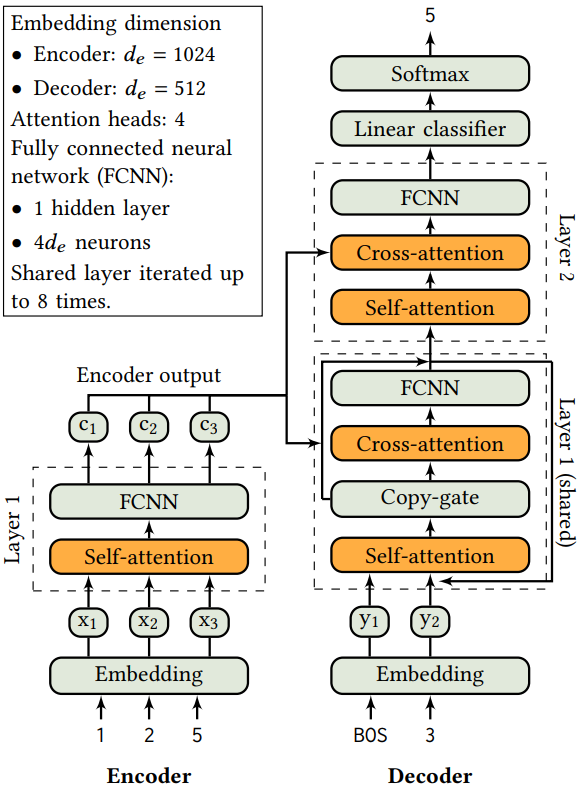
\includegraphics[width=.4\textwidth, height=.4\textwidth]{ML/Transformer_model.png}
    \caption{Transformer architecture used to solve the LWE problem taken from \cite{wenger2022salsa}}
    \label{fig:transfromer_arch}
\end{figure}

The overall attack methodology proceeds in three stages: data preprocessing, model training and  secret recovery as shown in the figure \ref{fig:attack_methodology}. The overall attack using ML proceeds as follows: Given $m$ LWE samples of fixed dimension $n$, modulus $q$ and with secret sampled from distribution $\chi$ the attack proceeds by performing following task in each of the above steps as follows.
\begin{figure}
    \centering
    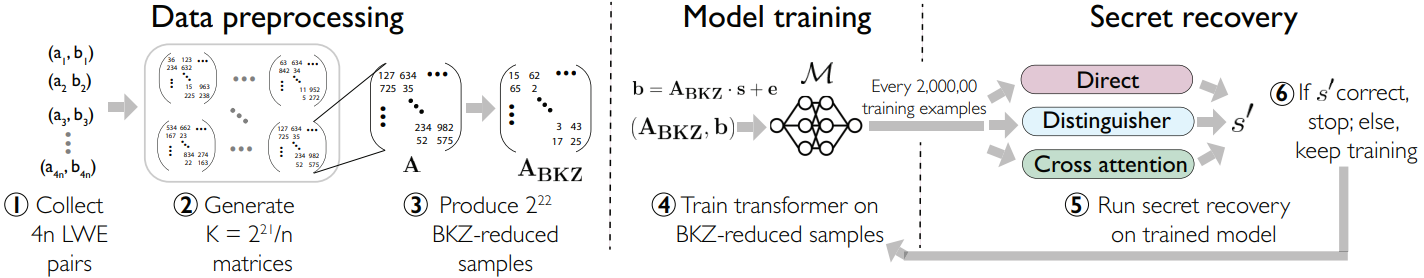
\includegraphics[width=\textwidth, height=.2\textwidth]{ML/Attack_methodology.png}
    \caption{Overall attack methodology using ML taken from \cite{li2023salsa}}
    \label{fig:attack_methodology}
\end{figure}

\paragraph{Data preprocessing}: In this step, $n$-LWE sample $(\textbf{a}_i,b_i)$ are subsampled from a pull of $m=4n$ samples to construct a matrix $\textbf{A}$ using $\textbf{a}_i$'s and to form a vector $\textbf{b}$ from $b_i$'s. Later, matrix $\textbf{A}$ is processed using some basis-reduction algorithm like LLL \cite{} or BKZ \cite{}; the same operations are performed on the vector $\textbf{b}$. The motivation behind the same is to obtain LWE samples with smaller coefficients to feed to the ML model, which performs better when the LWE sample entries are small.

This process is repeated to create $2^{21}/n$-matrices from ${4n \choose n}$ unique possible matrices. The subsampled $2^{21}/n$-matrices after reduction results in about $2^{22}$ (4 million) reduced LWE pairs. In general, the subsampled matrix contains duplicate rows, but after reduction, experimentally, no duplicate rows have been observed in the $4$ million created samples for dimension $n \geq 150$.

After sampling and recombination of LWE samples, lattice reduction is carried out on the lattice $\Lambda_i$ constructed using $n$ LWE samples $(\textbf{a},b)$ to make the LWE samples more amenable to the model training \cite{wenger2022salsa}. Subsample $n$-LWE sample to construct a lattice $\Lambda_i$ as shown below.
\begin{align*}
    \Lambda_i &= \begin{bmatrix}
                \omega \cdot \textbf{I}_n \hspace{1em} &  \textbf{A}_i  \\
                0                         \hspace{1em} &  q \cdot \textbf{I}_n
            \end{bmatrix}
\end{align*}
Here $n \times n$ matrix $\textbf{A}_i$ is constructed from $n$-LWE samples, $\textbf{I}_n$ is the identity matrix and $\omega \in \mathbb{Z}$ is the error penalization parameter.

Using lattice reduction algorithm BKZ to lattice $\Lambda_i$ transforms it by transformation $[\textbf{R}_i \hspace{1em} \textbf{C}_i]$, in such a way that the output matrix $[\omega \cdot \textbf{R} \hspace{1em}  \textbf{RA}+q\textbf{C}]$ will have $2n$ rows with small norms. Furthermore, the matrix $q\textbf{C}$ will add an integer multiple of $q$ to each entry in $\textbf{RA}$, so that all entries will be in the range $(-q/2,q/2)$.

\begin{align*}
    [\textbf{R}_{2n \times n} \hspace{1em} \textbf{C}_{2n \times n}]
    \begin{bmatrix}
        \omega \cdot \textbf{I}_n \hspace{1em} &  \textbf{A}_{n\times n} \\
        0                         \hspace{1em} &  q \cdot \textbf{I}_n
    \end{bmatrix} &=
    \begin{bmatrix}
        \omega \cdot \textbf{R}  \hspace{1em} &  \textbf{RA}+q\textbf{C}
    \end{bmatrix}
\end{align*}
Computed linear transformation $\textbf{R}$ is later applied to vector $\textbf{b}$ to create a new  LWE instance $(\textbf{RA},\textbf{Rb})$ with the same secret $\textbf{s}$ but reduced error $\textbf{e}'=\textbf{Rb}-\textbf{RA} \cdot \textbf{s}=\textbf{R}(\textbf{b}-\textbf{A}\cdot\textbf{s})=\textbf{Re}$ ($\textbf{e}=\textbf{b}-\textbf{A}\cdot \textbf{s}$). Thus, the final error depends on matrix $\textbf{R}$ values, and all values are computed under modulo $q$.

To control error amplification, parameter $\omega$ has been used. As stated earlier, BKZ computes $\textbf{R}$ and $\textbf{C}$ so that the norms of the row $[\omega \cdot \textbf{R} \hspace{1em}  \textbf{RA}+q\textbf{C}]$ are small. Large $\omega$ encourages small entries in the rows of $\textbf{R}$ but hinders the norm reduction of $\textbf{RA}+q\textbf{C}$ limiting the norm reduction of $\textbf{A}$ coordinates. In short, the choice of $\omega$ controls the trade-off between the reduction of $\textbf{a}$ we can achieve and the amount of additional noise injected in the transformed samples.

Recently, in \cite{li2023salsaver}, it has been observed that re-arranging the rows of lattice $\Lambda_i$ as
\begin{align*}
    \Lambda'_i &= \begin{bmatrix}
                0                         \hspace{1em} &  q \cdot \textbf{I}_n \\
                \omega \cdot \textbf{I}_n \hspace{1em} &  \textbf{A}_i
            \end{bmatrix}
\end{align*}
Results in a reduced number of operations needed for lattice reduction and allows BKZ to run with lower floating point precision. These two improvements cut the pre-processing time significantly.


\paragraph{Model training}: In this step the reduced LWE samples obtained from data preprocessing step above enters into the model training stage. For better understanding model training can be subdivided into following subcategories: data encoding, model architecture choice, and the training itself.

In data encoding step LWE samples are encoded in base $B$, as a sequence of tokens in $\{0, \cdots, B-1\}$. After encoding the coordinates of $\textbf{a}$ and $b$ are represented as two digit numbers in base $B$. Experiments performed for varying values of $B$ revels that large value of $B$, which limits the most significant digit of $a_i$ and $b$ to a small number of values provide better performance. Thus for all experiments value of $B$ is set to $B=\lfloor q/k \rfloor$ with $k=2\cdot \lceil \frac{n}{100}\rceil + 2$. However this creates a problem for large dimensions this is because large values of $q$ and $B$ results in large token vocabularies and is difficult to learn for the transformers with limited LWE samples. Mitigation of this is obtained by using encoding of the lowest digits of $\textbf{a}$ and $b$ into $B/r$ buckets of size $r$. Usually, $r$ is chosen in such a way that the  overall vocabulary size $B/r< 10,000$. Furthermore, usage of buckets helps training of models for large value of $n$ but have an impact on the loss of precision in the values of $\textbf{a}$ and $b$. However, it is believe that the impact on performance is limited, as it only affects the low bits of $\textbf{a}$ and $b$, which are anyways the most corrupted by LWE error.

The model architecture used for training and later to predict the value of $b$ is shown in figure \ref{fig:transfromer_arch}. The model, inspired from \cite{vaswani2017attention}, is a seq2seq model composed of two transformer stacks-- an encoder and a decoder, connected by a cross-attention mechanism. Here, the encoder gets the encoded discrete LWE samples as an input. The input sequence is first projected over a high-dimensional space (dimension $d=1024$ to be precise) by a Linear Embedding Layer with trainable weights (the embedding is learned during training, and initial embedding is generated using some seed). The resulting sequence is later processed by a single-layer transformer: a self-attention layer with four attention heads and a Fully connected neural network (FCNN) with one hidden layer of 4096 neurons.

The decoder is an auto-regressive model, which predicts the next token in the output sequence, given the already decoded output and the input sequence processed by the encoder. The decoder is provided a beginning of sequence token (BOS) and predicts $b_1^*$, the first digit of $b$. It is then fed the sequence BOS, $b_1^*$, and decoding proceeds until the end-of-sequence token (EOS) is output. The decoder input tokens are encoded as $512$-dimensional vectors via a trainable embedding. The decoder is made up of two layers. First, a shared layer, which is iterated through 8 times, feeds layer output back into its input. This recurrent process is controlled by a copy-gate mechanism, which decides whether a specific token should be processed by the shared layer or copied as is, skipping the next iteration. After eight iterations, the output of the shared layer is fed into a “regular” transformer layer. Finally, a linear layer processes the decoder output and computes the probability that any word in the vocabulary is the next token. The largest probability is selected via a softmax function.

As shown in the figure the decoder is connected to the encoder via a cross-attention mechanism with 4 attention heads. Speaking in more details, in each head, the output of the encoder $E=(E_i)_{i\in \mathbb{N}_l}$ ($l$ being the input sequence length) is multiplied by two trainable matrices, $W_k$ and $W_v$ , yielding the Keys $K$ = $W_k E$ and Values $V$ = $W_v E$. The 512-dimensional vector to be decoded, $D$, is multiplied by a matrix $W_Q$, yielding the Query $Q=W_Q D$. The $l$ scores are calculated from the query and keys as
\begin{align*}
    scores(E,D) = Softmax( (W_Q D) (W_K E)^T)
\end{align*}
The score calculated above measures the importance of each encoder input element when decoding $D$  i.e. while computing $b$. Usually, the cross-attention value for each head is the dot product of scores and values. Values of different heads are latter processed by a final linear layer. Cross-attention scores quantify the relation between input positions and output values. Picante uses them to recover the secret bit by bit.

The model $\textbf{M}$ discussed above is later used to predict $b$ from encoded $\textbf{a}$. The model $\textbf{M}$ treats it as a supervised multi-classification problem, by minimizing the loss function:

\begin{align*}
    min_{\theta \in \Theta} \sum_{i=1}^{N} \sum_{j=1}^{K} \sum_{k=1}^{V} \textbf{1}[y_i[j]=k-1] \frac{e^{\textbf{M}(x_i)[j,k]}} {\sum_{k'=1}^V e^{\textbf{M}(x_i)[j,k']}}
\end{align*}
The different parameters used in the model above are as follows: $\textbf{M}(x_i) \in \mathbb{R}^{K\times V}$ are the model logits evaluated at $x_i, \theta \in \Theta$, $N$ is the training sample size, $K=2$ is the output sequence length and $V=B/r$ is the vocabulary size.

To get prediction of $\textbf{M(a)}$ near to the ground truth $b$, the cross entropy needs to be minimized over all tokens in the output sequence. Bath traing is used to train the model with batch size $n_b=128$ examples. Furthermore, the cross-entropy loss $\textbf{L}(\textbf{M},\textbf{a},b)$ is computed over all batch examples and gradient $\nabla \textbf{L}$ are calculated with respect to the model parameters. Model parameters are later updated using the Adam optimized by $lr \nabla \textbf{L}$. $lr$ here represents the learning rate and is initially set to $10^{-5}$, except during the $1,000$ first optimizer steps, where it is increased linearly from $10^{-8}$ to $10^{-5}$. In the model used for computing the unknown secret, the model performance is evaluated after every epoch (epoch=$2$ million samples) on a held-out samples and secret recovery is tried if the it fails then another epoch begins.

%above are later encoded in base B and are used to train the model $M$. Training with sufficiently large number of LWE samples results in model $M$ being learned to predict $b$ from $\textbf{a}$. Usually, model training proceeds in epochs, each using 2 million samples. The 4 million training data are shuffled randomly every two epochs.

\paragraph{Secret recovery}: At the end of each epoch, the ML attack tries to recover the secret using different techniques. The intuition behind the same is that if the model $\textbf{M}$ can predict $b$ from $\textbf{a}$, then model $\textbf{M}$ somehow "knows" the secret $\textbf{s}$ and we can recover it from the model by enquiring the model. For secret recovery three techniques: direct, distinguisher, and cross-attention have been used. The different secret recovery techniques can be used standalone and can also be used in combination to recover the secret. Below we will discuss each techniques in more detail.

\paragraph{Direct secret recovery}: The idea behind this technique is to leverage the trained transformer's ability to generalize on inputs not seen during the training. To be precise, the training model is evaluated on special vector $\textbf{a}$ with one non-zero coordinate: $\textbf{a}=K\textbf{e}_i$ with $\textbf{e}_i$ the $i$-th standard basis vector and $K\in \mathbb{Z}_q$. For such vectors, since $b=\textbf{a}\cdot\textbf{s}+e$, and $\textbf{e}$ is small, $b\approx K$ if the $i$-th bit in the secret $\textbf{s}_i=1$and $b \approx 0$ otherwise. Usually, different $K_j$ are chosen, and the transformer is evaluated on $K_j\cdot e_i$ for $i=1,\cdots,n$, identifying potential $1$-bit in secret and producing a secret guess for each $K_j$.

\paragraph{Distinguisher secret recovery}: The general idea behind this technique is that if the $i$-th bit of the secret $s_i=0$ and $\textbf{e}_i$ is the $i$-th standard basis vector, then the model should predict close values for $\textbf{a}$ and $\textbf{a}+K .\textbf{e}_i$. Here the value of $b'=\textbf{M}(\textbf{a}+K \cdot \textbf{e}_i)$
is compared with $\textbf{M(a)}$. The rest remains the same; set the secret bits corresponding to the $h$ highest-scoring secret bits to $1$ and the rest to $0$.

\paragraph{Cross-Attention secret recovery}: This technique aims to recover the secret from the parameters of $\textbf{M}$ by leveraging the cross-attention scores of the first decoder layer. Intuitively, the cross-attention score measures the relevance of input tokens in the computation of $b$. Putting it simply, the coordinates of $\textbf{a}$ that correspond to the $0$ bits of $\textbf{s}$ have no impact on $b$, while the coordinates associated with the $1$ bits in $\textbf{s}$ have an impact proportional to their value in the calculation of $b$. Thus, we should get high-attention scores corresponding to the input positions $1$'s in the secret.


LWE problem is broadly categorized into three categories:
\begin{itemize}
    \item Easy: These are the category of LWE problem instances that are solvable via exhaustive search.
    \item Medium-to-hard: These category of LWE problem instances requires significant/unrealistic resources even for best known available attacks.
    \item Standardized: These category of LWE problem are the LWE problems that are believed secure or are not affordable to beak in a reasonable time using current computing facilities.
\end{itemize}

ML based attacks can break the Medium-to-hard LWE problems outperforming the lattice reduction attacks such as uSVP. However, it is still fur behind in breaking the LWE schemes standardized by NIST, which uses larger dimensions, smaller moduli $q$, and general secret distributions.



% !TeX root = ../sameplaper.tex
% !TeX spellcheck = en_US

\chapter{Project Meetings} %Project Soteria Attack Scenario}
\setcounter{section}{0}


\section{Weekly Meeting}
% subsection{Meeting With Ana and Flavio}

\begin{itemize}
    \item When a user forms a query the query can be sends for query computation in two ways
          \begin{enumerate}
              \item Users query is sent using user's metadata for query computation  to the server with users metadata. In this case authenticity of the user is verified from the user database stored in the server and same for the the service validity check. After successful authentication and verification the query computation is performed which is later decrypted and decoded and the obtained final plain result is forwarded to the user who submitted the query. This method have a drawback of maintaining users database on the server side and similarly for the service information of the users service information have to be stored. As more users registers in the institutions it have to constantly update and maintain the database. Similarly when a users registration have been withdrawn then it have to be updated into the server side which creates heavy overload on the server side.
              \item Users query is sent with institutions metadata. Here when a user asks for a query request users authenticity is verified in the client side portal itself. On successful authentication users are provided query encryption facility. On successful query encryption users query is sent with the institutions metadata storing the users metadata on the client side portal. Server side performs institution authentication and service validation of institution. On successful authentication and verification query computation is performed. The result is forwarded to the institution. Institution identifies the user who generated the query request from its database and sends it query result to the corresponding user.
          \end{enumerate}
    \item HE query result can be stored in one of the two places:
          \begin{enumerate}
              \item Server side: Query result is stored in the server side for pre-decided time interval. Before the time expires the query requester have to access the result else result is deleted from the database.
              \item Client side: Query result is stored in some database. The result remains in the database until the user access it. There is no time associated with the query result lifetime. Thus the user don't have to bother about the expiry of the query result.
          \end{enumerate}
    \item For data safeguard data diode can be used. A data diode is the one in which data only moves in one direction. Data diodes are hardware-based devices with two nodes or circuits—one send only and one receive only—that allow the flow of data in one direction only, from a source to a destination. It is also called as a unidirectional network. Firewalls can be used instead of data diodes.
    \item Force deviation and the system behaviour
    \item Memory overflow attack
    \item Targeted attack
    \item Network admin and Database admin should be completely separate and should never combine the two. Combination of these unknowingly may make the system vulnerable using the combination of attack techniques and leakages.
    \item System logs should be stored safely so that if something wrong happens then it can be analyzed later. However prevention is better than cure.
    \item What are the different type of denial of service attack?
    \item Attack on front end of the query?
    \item Attack on the underline messaging system?
    \item Can we quantify the risk associated with the HE deployment?
    \item For query encryption:
          \begin{enumerate}
              \item Initially QU have cleartext. From this prepare query predicate for a query.
              \item Perform encoding.
              \item Perform query encryption.
              \item Combination phase: In this phase lots of queries are combined with encryption predicates.
          \end{enumerate}
    \item When data flows from the high security domain to low security domain then in this case it creates a security problem. Thus this must be taken care of.
    \item When data flows from low security domain to high security domain data gets classified thus disposing of data becomes a real problem. Thus to handle disposing of data from low security domain to high security domain must be taken care of using proper procedures.  To handle such scenarios help of some third party or proxy organization is taken who checks security of on behalf of host party. This task is usually outsourced to avoid security breach.
    \item When a query comes to the server for query computation---validation or query well formness is checked before sending it for query computation. In this step following checks are performed:
          \begin{enumerate}
              \item Query is right or not
              \item Valid for user or not.
              \item Metadata came with the query is correct or not.
              \item Service parameters are correct or not.
          \end{enumerate}
    \item Client laptop by design is dishonest.
    \item Edge device is vulnerable and dishonest (Honest but curious are not trustworthy)
    \item Attack can have multiple actors taking part of attack to control viz. MITM attack.
    \item Attack can be on the protocol itself viz. TLS1.3
    \item Write separate user authentication from that of HE. Use whatever technology available today for FHE threat flow.
    \item Use different technologies to get verifiable computation.
    \item User has only decrypted and decoded result.
    \item Different institutions may have different (pk,sk) pair, Keys are kept by the isntitutions and are never exposed to anyone.
    \item User authentication should be backed up by the technologies available today viz. HTTPS, PKI etc.
    \item Mostly attacks are from client side including the passive attacks.
    \item Key management
    \item There is no algorithmic way of risk evaluation. Matrix for risk analysis some sort of inference if we can provide.
    \item Combine different technology and try to measure the risk.
    \item Explore the vulnerability of the client side.
    \item How to perform FHE key management
    \item User is never trusted in the deployment setting
\end{itemize}
\paragraph {$9^{th}$ march}
\begin{itemize}
    \item Our FHE computation assumes that the database is encoded and not encrypted.
    \item Next assumption: The server side owns the database.
    \item Thus, the database can be encrypted using AES and decrypted and computed in TEE.
    \item Our query comes in an encrypted form encrypted with a BGV encryption scheme.
    \item Focus on Bottom-up analysis rather than Top-down analysis viz. focus on CCA security, CPA security with an assumption that adversary is an Honest But Curious (HBC).
    \item Focus on how FHE computation is done, the vulnerability in FHE computation
    \item Write a list of FHE assumptions and security parameterization
    \item If assumptions do not hold true, then the list of potential threats that a bed actors can do
    \item If assumptions do not hold true, then what happens in CPA and CCA scenario
    \item Use of decryption oracle to decrypt result, can adversary also gets the decrypted result before decoding. In such scenarios, what should we do?
    \item Use a little bit of error and check the behavior of the client or the user. In doing so, what information can be learned?
    \item Explore ciphertext injection attack.
    \item Preserve the depth of the computation.
    \item Explore the equilibrium of the cost of preserving and the cost of attacking.
    \item Design system in such a way that even if an attacker breaks the system, the benefit of breaking the system should be same as that of the resources invested. In sort in gain for the attacker.
    \item Make a table and show what may cause what attack and its vulnerabilities.

    \item Consider FHE computation separately, separate from key generation and ciphertext generation
    \item Vulnerability assumptions for the HBC FHE computation setting
    \item What HBC server can do to the intermediate data
          \begin{itemize}
              \item Corrupt the computation
              \item Corrupt the values
              \item Deviation from the computed values by known quantity to know the user behavior and use this information to get side channel information
          \end{itemize}

\end{itemize}
\paragraph{6th April}
\begin{itemize}
    \item Vulnerabilities of deployment of HE
    \item Vulnerabilities of the encryption schemes
    \item Mention the attacks present in Martin's paper
    \item Potential attacks for deployment (decryption attacks like those proposed by Li and Miccancio)
    \item Analyze deployment
    \item Analyze by the encryption schemes
    \item Lattice attack on encryption schemes
    \item Mitigation for the deployment (Create the content in such a way that deployment can avoid the vulnerabilities present in the encryption scheme)
    \item Separate chapter-wise each of the topics
    \item After writing the chapters, connect the chapters.
    \item Security of FHE
    \item Attacks
          \begin{itemize}
              \item Key recovery attacks
              \item Attacks to break the key
              \item Attacks to break the homomorphic computation
              \item Side channel attacks
              \item Noise level left in the ciphertext
              \item When a user stops decryption of the ciphertext due to too much noise
              \item Man-in-the-middle type of attacks
              \item Other types of attacks like
                    \begin{itemize}
                        \item When the public keys are available to the user?
                        \item Encoding, parameter choices, Noise sampling, Encoding, Public key, etc are known to the attacker
                    \end{itemize}
          \end{itemize}
    \item Mitigation of attacks and corruption of ciphertext.
    \item Corruption of the final ciphertext should not be possible
    \item Error distribution and Noise distribution
\end{itemize}
\paragraph{19th June}
\begin{itemize}
    \item Study about dimension leakages
    \item Dimension leakages in case of HE
    \item size of database and entries leakages in case of HE
    \item plaintext parameter leakages in case of HE
    \item For loops in cotrol variable in case of HE
    \item In case of deployment leakages of data information and algorithms
    \item What is confidential in case case of data viz., dimension,for etc.
    \item Is there any infomration leakages will be there in case of padding with zero to the data used for encryprion
    \item Algorithmic leakages and recommandations
    \item What kind of information leakages will be there in case of leakages in the BGV and CKKS encryption schemes
    \item Or puttng otherwise, how  frequently the the keys should be refresh and Ciphertext as well
    \item Write schemes based on LWE NTRU and AGCD
\end{itemize}

\paragraph{26th June}
\begin{itemize}
    \item Summarized Our research objective to Alex
    \item Decided to target the SOK paper on Homomorphic Encryption to S\&P 2023 Dec 6 deadline and if we can not make it then try for PETS 2024
\end{itemize}




\section{Attacks on entities associated to HE deployment}

\subsection{Client-Side Components}
\begin{enumerate}
    \item User
          \begin{itemize}
              \item Opens the Query Service Client and requests the query service
              \item Sends its query to the query service client
          \end{itemize}
    \item Query service client
          \begin{itemize}
              \item Authenticates the requested service
              \item Extracts query predicates and builds the query
              \item Encrypts the query predicate and sends it to the Service Query portal
          \end{itemize}
    \item Encrypted Result store
          \begin{itemize}
              \item Encrypted result is decrypted in the Trusted Execution Environment
              \item Result is received by the query service client which sends result to the corresponding query user
          \end{itemize}
\end{enumerate}

\subsection{Server-Side Components}
\begin{enumerate}
    \item Service Query Portal
          \begin{itemize}
              \item Authenticates user and institution using
                    \begin{itemize}
                        \item User at Institution
                        \item Query Id
                        \item Query Data
                        \item Job Id
                    \end{itemize}
              \item Transmits user query to query engine
          \end{itemize}
    \item Service registry
          \begin{itemize}
              \item Validates institutions and possibly users
              \item Validates that the Institution/user is authorized to ask the requested service.
              \item On successful authorization forwards the users metadata
          \end{itemize}
    \item Service KMS
          \begin{itemize}
              \item Stores Institution id with Public and Evaluation keys (May be encrypted with HSM using symmetric key encryption like AES)
              \item Provides (institution specific) Evaluation Keys
              \item Encoding techniques is not known to the KMS
          \end{itemize}
    \item Data Store
          \begin{itemize}
              \item Stores database in cleartext or plaintext
              \item Query predicates are searched in the database for results
          \end{itemize}
    \item FHE Query Engine
          \begin{itemize}
              \item Does homomorphic computation using:
                    \begin{itemize}
                        \item User metadata
                        \item Institution eval keys
                        \item Data store
                    \end{itemize}
          \end{itemize}
    \item Encrypted Results Store
          \begin{itemize}
              \item Receives encrypted results from query engine
              \item Allows retrieval of results by relevant institution
          \end{itemize}
\end{enumerate}

\subsection{Passive Risks: leakage when components follows the protocol?}

\textcolor{blue}{Blue highlights indicate risks when component can observe client behaviour. (CCA)}

\textcolor{red} {Red highlights indicate risks associated with corrupted ciphertexts, and the possibility of ciphertext verification attacks. (CVA)}
\begin{enumerate}
    \item Service query portal
          \begin{itemize}
              \item Learns frequency of queries by institution
              \item Knows which institutions are valid
              \item Knows which users are valid at a given institution
              \item Processes a query
                    \begin{itemize}
                        \item Knows the query predicates
                        \item Sees ciphertext of query predicate
                    \end{itemize}
          \end{itemize}
    \item Service registry
          \begin{itemize}
              \item Learns frequency of queries by institution and by user
              \item Learns user/institution meta data
                    \begin{itemize}
                        \item Learns institution security level
                        \item Learns dimension of user input?
                        \item Type of service user/institution is registered for?
                    \end{itemize}
          \end{itemize}
    \item Service KMS
          \begin{itemize}
              \item Learns frequency of queries by institution
              \item Sees Eval keys: has access to a large quantity of ciphertexts
              \item Keys can be encrypted using the HSM can only see the encrypted Eval keys
          \end{itemize}
    \item Data Store
          \begin{itemize}
              \item \textcolor{blue}{If can observe client behaviour, may be able to infer (something about) user’s data: however unclear whether this component knows which request corresponds to which user.}
              \item If plaintext (not cleartext) learns something about parameters of schemes used
          \end{itemize}
    \item FHE Query Engine (closest to monolithic HE server from current modelling)
          \begin{itemize}
              \item Learns frequency of queries by institution
              \item Receives a query: same risks as service query portal
                    \begin{itemize}
                        \item Learns the query predicates
                        \item Sees ciphertext of query predicates
                    \end{itemize}
              \item Learns user/institution meta data: same risks as service registry
                    \begin{itemize}
                        \item Learns service security level
                        \item Size of evaluation key / query predicates size
                        \item Learns dimension of user input.
                        \item Type of service user/institution is registered for?
                    \end{itemize}
              \item Receives data: same risks as data store
              \item Receives eval keys: same risks as service KMS
              \item Sees result ciphertext
              \item additional risks come from information seen in conjunction
                    \begin{itemize}
                        \item Has query ciphertext AND eval keys
                        \item \textcolor{blue}{Sees database AND knows specific user}
                    \end{itemize}
          \end{itemize}
    \item Encrypted results store
          \begin{itemize}
              \item Understands frequency of queries by institution and by user from retrieval
              \item Sees result ciphertext
                    \begin{itemize}
                        \item Can infer something about query evaluation circuit
                        \item \textcolor{blue}{Can infer about ciphertext decryption from user/institution behaviour}
                    \end{itemize}
          \end{itemize}
\end{enumerate}


\subsection{Active Risks: leakage when components deviate from the protocol description?}
\textcolor{blue}{Blue highlights indicate risks when component can observe client behaviour. (CCA)}

\textcolor{red} {Red highlights indicate risks associated with corrupted ciphertexts, and the possibility of ciphertext verification attacks. (CVA)}
\begin{itemize}
    \item Service Query Portal
          \begin{itemize}
              \item Denial of service attacks
              \item Can substitute or modify query data ciphertext, possibly \textcolor{blue}{leading to decryption oracle creation} and/or \textcolor{red}{corrupted ciphertexts}
              \item Can change query logic
              \item Can swap institution ID, leading to \textcolor{red}{corrupted ciphertexts}
          \end{itemize}
    \item Service registry
          \begin{itemize}
              \item Can change metadata, which can lead to \textcolor{red}{corrupted ciphertexts}
          \end{itemize}
    \item Service KMS
          \begin{itemize}
              \item Denial of service
              \item Corruption of eval keys, leading to \textcolor{red}{corrupted ciphertexts }
              \item Corruption of public encryption key, leading to \textcolor{red}{corrupted ciphertexts}
              \item \textcolor{blue}{Can generate valid ciphertexts using public keys}
          \end{itemize}
    \item Data Store
          \begin{itemize}
              \item Denial of service
              \item Can modify database to try and infer something about query data \textcolor{blue}{by observing client behaviour}
              \item Can modify database to ensure decryption failures, leading to \textcolor{red}{corrupted ciphertexts}
          \end{itemize}
    \item FHE Query Engine
          \begin{itemize}
              \item All risks previously covered, and
              \item Can reply chosen query request by valid ciphertext
              \item Can generate any request and encrypt it
              \item Can corrupt the ciphertext for the correct query
              \item Can evaluate a different circuit other than the one requested
              \item Can generate \textcolor{blue}{valid ciphertexts associated to the query ciphertext}
              \item Can produce corrupt result
          \end{itemize}
    \item Encrypted Results Store
          \begin{itemize}
              \item Can use ciphertext received metadata/context to generate a \textcolor{red}{corrupted ciphertext}
              \item Can generate valid ciphertexts with known relationship to target by e.g. adding plaintexts and \textcolor{blue}{observe client behaviour to create a decryption oracle}
          \end{itemize}
\end{itemize}

 %Meeting details

% !TeX root = ../sameplaper.tex
% !TeX spellcheck = en_US

\chapter{Attack Classification}
\setcounter{section}{0}


Categorization of attacks
Attacks can be mainly categorized into

\section{Passive attacks}
\begin{itemize}
    \item Here all the components follow the protocol however, they passively keep track of all steps followed and any private information that can be gained from it.
    \item To avoid such attacks the system must be designed that leaks as minimum information as possible.
\end{itemize}

\section{Active attacks}
\begin{itemize}
    \item In this attack setting the components can deviate from the protocol and behave independently resulting into even wrong computation.
    \item These types of attacks are usually hard to take care of.
\end{itemize}

\section{Side Channel Attacks}
\begin{itemize}
    \item These are the attacks that are based on the side information that are gathered when the protocol or the algorithm is implemented and used.
    \item Timing information, power consumption electromagnetic leaks and sound analysis are the examples of side information’s that are exploited to facilitate the side-channel attacks.
\end{itemize}

\section{Denial of Service attack}
\begin{itemize}
    \item These are the attacks meant to shut down a machine or network, making it inaccessible to its intended users.
    \item DoS attacks are usually accomplished by flooding the target with traffic or sending it information that triggers a crash.
    \item In both instances, the DoS attack deprives legitimate users of the service or resource they expected.
\end{itemize}

\section{Insider attack}
\begin{itemize}
    \item These are the attackers who have access to the inside leakage and can mount attack based on the information they have.
\end{itemize}

\section{Combination of attacks}
\begin{itemize}
    \item In this attack techniques different attack gets combined and uses the combined information to extract the unauthorized information.
\end{itemize}

 %Meeting details


% !TeX root = ../sameplaper.tex
% !TeX spellcheck = en_US

\chapter{Homomorphic Encryption Deployment}
\setcounter{section}{0}

\section{HE deployment}
% Software that are used in real life applications face a variety of threats and challenges and also changes with the change of technology. A threat can arise form outside as well as from inside. An attacker can disable the system entirely or may get sensitive information from the system using the leakage of sensitive information leaked during computation. Result of this may result ino diminishing the users trust for the system. Thus threat modeling/analysis plays an important role to counter measure the threat from taking advantage of system design flaws resulting into leaking sensitive information. There are couple of threat modeling techniques available in the literature \cite{shevchenko_2018}. Identification of a suitable threat model for a particular application depend upon specific needs of the project.

Softwares that are used in real-life applications face a variety of threats and challenges and also changes with the change of technology. A threat can arise from outside as well as from inside. An attacker can disable the system entirely or may get sensitive information from the system using the system's leakage of sensitive information leaked during computation, which the attacker can use for financial gain or to disable the system altogether. This results in diminished users' trust in the system and may also result in considerable losses to the business. Thus, threat modeling or analysis plays an essential role in countering  system design flaws, which may result in the leakage of sensitive information. Several threat modeling techniques are available in the literature \cite{shevchenko_2018}. However, identifying a suitable threat model for a particular application depends on the project's specific needs.

Here we will use the STRIDE \cite{The_Threat_Model} model to investigate possible attacks in each entity/component and determine its mitigation techniques. By building a data flow diagram (DFD), STRIDE is used to view the system design details. STRIDE, a mnemonic of the terms Spoofing, Tempering, Repudiation, Information disclosure, Denial of Service, and Elevation of privilege, can be applied to any cyber-physical system. Figure \ref{fig:basic_dfd} shows the DFD drawn for studying STRIDE of HE deployment. As shown in the figure, each modular entity is considered separately, and its security and leakages are investigated individually.

Furthermore, deployment of HE can be divided into two parts. The first part focuses on creating a secure communication channel between the parties involved. For creating a secure communication channel between the user and the client query portal, we have suggested using public key infrastructure (PKI) \cite{PKI}. Figure \ref{fig_public_key_infrastructure} shows the use of PKI for secure electronic transfer of information of different kinds. PKI is usually required for activites where simple passwords are an inadequate authentication method and more rigorous proofs are required to confirm the identity of communicating parties involved so that some attacks like MITM can be avoided and to validate the information being transfered to the intended party.



%------------------------DFD starts here-------------------------------------------------
%Figure to show the TLS1.3 connection istablishment
\begin{figure}[!ht]
    \centering
    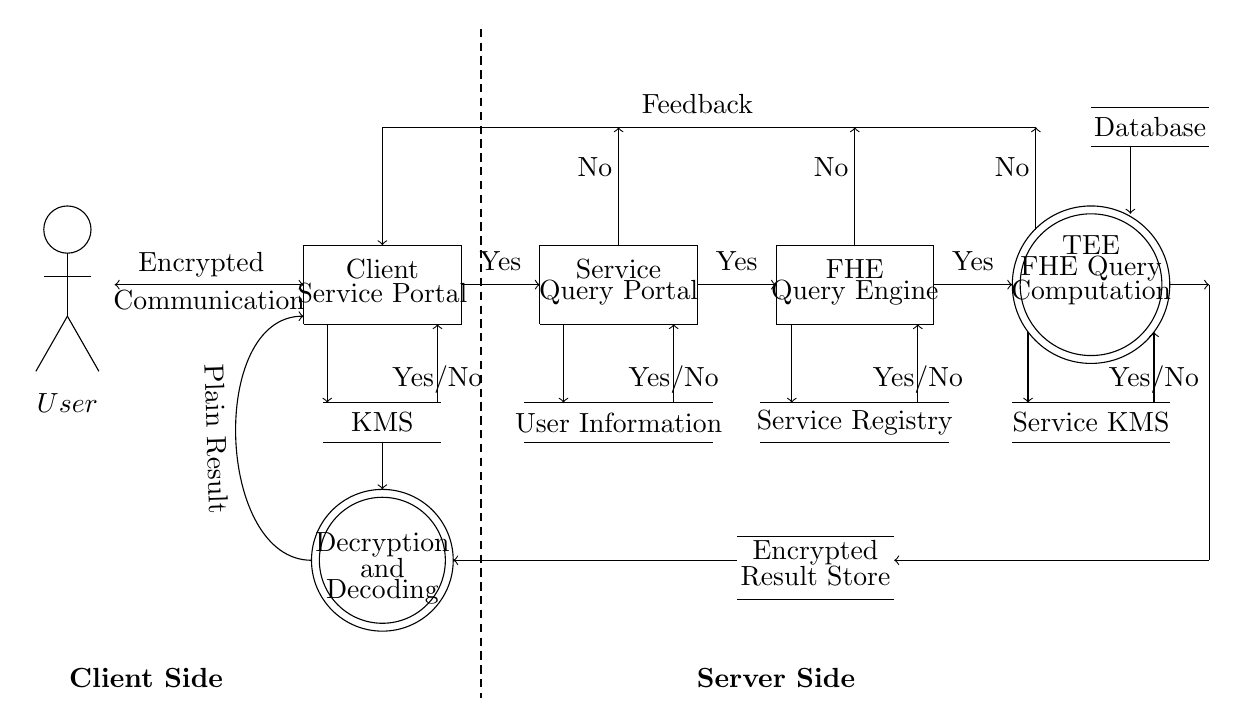
\begin{tikzpicture}

        %separating line between client and server
        \draw [thick , densely dashed] (-6.75,2.75) -- (-6.75,-5.75);
        \node at (-11,-5.5) {$\textbf{Client Side}$};
        \node at (-3,-5.5) {$\textbf{Server Side}$};

        %Drawing an User
        \draw (-12,.2) circle [radius=.3]; %head
        \draw (-12.3,-.4) -- (-11.7,-.4);  %hands .4 -.4   .7 .7
        \draw (-12,-.1) -- (-12,-.9); %spinal cord  0 0    .4 1.4
        \draw (-12,-.9) -- (-12.4,-1.6); %left leg 0 .4     1.4 2.2
        \draw (-12,-.9) -- (-11.6,-1.6); %right leg 0 -.5    1.4  2.2
        \node at (-12,-2) {$User$}; %0          -1.5


        % Client Service Portal
        \draw (-9,-1) -- (-7,-1) -- (-7,0) -- (-9,0) -- (-9,-1);
        \node at (-8,-.3) {Client };
        \node at (-8,-.6) {Service Portal};

        %connecting arrow between user and client query portal
        \draw [<->](-11.4,-.5) -- (-9,-.5);
        \node at (-10.3,-.25) {Encrypted};
        \node at (-10.2,-.7) {Communication};


        %KMS Database drawing
        \draw (-8.75,-2.5) -- (-7.25,-2.5);
        \draw (-8.75,-2) -- (-7.25,-2);
        \node at (-8,-2.25) {KMS};

        %Connecting line between KMS and client query portal
        \draw [<-](-8.7,-2) -- (-8.7,-1);
        \draw [->](-7.3,-2) -- (-7.3,-1);
        \node at (-7.3,-1.7) {Yes/No};

        %Connecting line between clent service portal and service query portal
        \draw [->](-7,-.5) -- (-6,-.5);
        \node at (-6.5,-.2) {Yes};


        % Service Query Portal
        \draw (-6,-1) -- (-4,-1) -- (-4,0) -- (-6,0) -- (-6,-1);
        \node at (-5,-.3) {Service };
        \node at (-5,-.6) {Query Portal};

        %User information Database drawing
        \draw (-6.2,-2.5) -- (-3.8,-2.5);
        \draw (-6.2,-2) -- (-3.8,-2);
        \node at (-5,-2.25) {User Information};

        %Connecting line between user information and service query portal
        \draw [<-](-5.7,-2) -- (-5.7,-1);
        \draw [->](-4.3,-2) -- (-4.3,-1);
        \node at (-4.3,-1.7) {Yes/No};

        %Connecting line between service query portal and FHE query engine
        \draw [->](-4,-.5) -- (-3,-.5);
        \node at (-3.5,-.2) {Yes};


        %FHE query engine
        \draw (-3,-1) -- (-1,-1) -- (-1,0) -- (-3,0) -- (-3,-1);
        \node at (-2,-.3) {FHE};
        \node at (-2,-.6) {Query Engine};

        %User Service registry Database drawing
        \draw (-3.2,-2.5) -- (-0.8,-2.5);
        \draw (-3.2,-2) -- (-.8,-2);
        \node at (-2,-2.25) {Service Registry};

        %Connecting line between FHE query engine and Service Registry
        \draw [<-](-2.8,-2) -- (-2.8,-1);
        \draw [->](-1.2,-2) -- (-1.2,-1);
        \node at (-1.2,-1.7) {Yes/No};

        %Connecting line between FHE query engine and TEE FHE query computation
        \draw [->](-1,-.5) -- (0,-.5);
        \node at (-.5,-.2) {Yes};

        %TEE FHE query computation
        \draw (1,-0.5) circle [radius=.9]; %head
        \draw (1,-0.5) circle [radius=1]; %head
        \node at (1,0) {TEE};
        \node at (1,-.3) {FHE Query};
        \node at (1,-.6) {Computation};

        %User Service KMS Database drawing
        \draw (0,-2.5) -- (2,-2.5);
        \draw (0,-2) -- (2,-2);
        \node at (1,-2.25) {Service KMS};

        %Connecting line between FHE query engine and Service Registry
        \draw [->](1.8,-2) -- (1.8,-1.1);
        \draw [<-](.2,-2) -- (.2,-1.1);
        \node at (1.8,-1.7) {Yes/No};

        %feedback system
        \draw []   (-8,1.5) -- (.3,1.5);
        \node at (-4,1.8) {Feedback};
        \draw [->]  (.3,.2) -- (.3,1.5); %TEE to line
        \node at (0,1) {No};

        \draw [->] (-2,0) -- (-2,1.5); %FHE query engine to line
        \node at (-2.3,1) {No};

        \draw [->] (-5,0) -- (-5,1.5); %Service query portal to line
        \node at (-5.3,1) {No};

        \draw [->] (-8,1.5) -- (-8,0); %Client Service portal to line



        %Database drawing
        \draw (1,1.75) -- (2.5,1.75);
        \draw (1,1.25) -- (2.5,1.25);
        \node at (1.75,1.5) {Database};
        \draw [->](1.5,1.25) -- (1.5,.4);

        %Computed Result send to Encrypted Result store
        \draw [<-](-1.5,-4)  -- (2.5,-4);
        \draw [-](2.5,-4) -- (2.5,-.50);
        \draw [<-](2.5,-.50)    -- (2,-.5);
        \draw [->](-3.5,-4)  -- (-7.1,-4);

        %Computed store in temporary database
        \draw (-1.5,-3.70) -- (-3.5,-3.70);
        \draw (-1.5,-4.5) --  (-3.5,-4.5);
        \node at (-2.5,-3.9) {Encrypted};
        \node at (-2.5,-4.2) {Result Store};


        %TEE computation
        \draw (-8,-4) circle [radius=.8]; %head
        \draw (-8,-4) circle [radius=.9]; %head
        \node at (-8,-3.8) {Decryption};
        \node at (-8,-4.1) {and};
        \node at (-8,-4.4) {Decoding};

        %Line from KMS to the Decryption and Decoding
        \draw [<-](-8,-3.1) --  (-8,-2.5);

        %Connecting line between decryption and decoding and client service portal
        \draw [ <- ] (-9,-.9)  to  [out=180, in=180  ,edge node={node [sloped,below]  {Plain Result}}] (-8.9,-4) ;




    \end{tikzpicture}
    \caption{Basic data flow diagram of FHE query computation}
    \label{fig:basic_dfd}
\end{figure}
%------------------------DFD ends here-------------------------------------------------
% \begin{figure}
%   \includegraphics[width=1.2\linewidth]{Diagrams/Basic_DFD.png}
%   \caption{Basic data flow diagram of FHE query computation}
%   \label{fig:basic_dfd}
% \end{figure}
%-------------------------------------------------------------------------------------


%------------------------PKI starts here onwards-------------------------------------------------
%Figure to show the TLS1.3 connection istablishment
\begin{figure}[!ht]
    \centering
    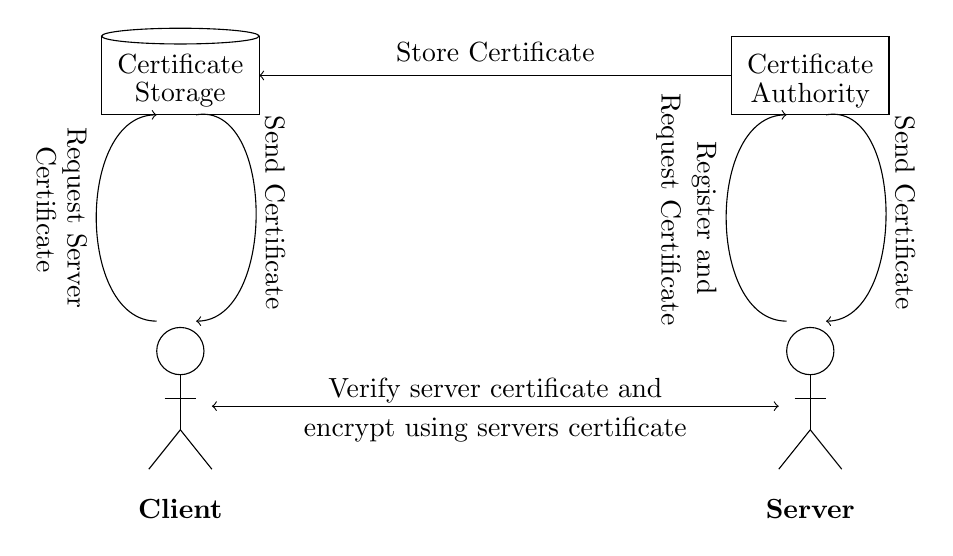
\begin{tikzpicture}

        %Drawing Client
        \draw (-12,0) circle [radius=.3]; %head
        \draw (-12.2,-.6) -- (-11.8,-.6);  %hands .4 -.4   .7 .7
        \draw (-12,-.3) -- (-12,-1); %spinal cord  0 0    .4 1.4
        \draw (-12,-1) -- (-12.4,-1.5); %left leg 0 .4     1.4 2.2
        \draw (-12,-1) -- (-11.6,-1.5); %right leg 0 -.5    1.4  2.2
        \node at (-12,-2) {$\textbf{Client}$}; %0          -1.5

        %Drawing Server
        \draw (-4,0) circle [radius=.3]; %head
        \draw (-4.2,-.6) -- (-3.8,-.6);  %hands .4 -.4   .7 .7
        \draw (-4,-.3) -- (-4,-1); %spinal cord  0 0    .4 1.4
        \draw (-4,-1) -- (-4.4,-1.5); %left leg 0 .4     1.4 2.2
        \draw (-4,-1) -- (-3.6,-1.5); %right leg 0 -.5    1.4  2.2
        \node at (-4,-2) {$\textbf{Server}$}; %0          -1.5

        %Connecting line between client and server x
        \draw [<->](-11.6,-.7) -- (-4.4,-.7);
        \node at (-8,-.5) {Verify server certificate and};
        \node at (-8,-1) {encrypt using servers certificate};


        %Certificate storage
        \draw (-13,3) -- (-11,3) -- (-11,4)  (-13,4) -- (-13,3);
        \draw (-12,4) ellipse (1cm and .1cm);
        \node at (-12,3.65) {Certificate};
        \node at (-12,3.25) {Storage};

        %Certificate authority
        \draw (-5,3) -- (-3,3) -- (-3,4) -- (-5,4) -- (-5,3);
        % \draw (-12,4) ellipse (1cm and .1cm);
        \node at (-4,3.65) {Certificate};
        \node at (-4,3.25) {Authority};

        %Line between certificate storage and Certificate Authority
        \draw [<-](-11,3.5) -- (-5,3.5);
        \node at (-8,3.8) {Store Certificate};

        %Line between Server and Certificate Authority
        % \draw [<->](-4,3) -- (-4,.4);

        %Connecting line between certificate storage and client
        % \draw [<->](-12,.4) -- (-12,3);

        %Connecting line between server and certificate authority
        \draw [ <- ]  (-12.3,3) to  [out=180, in=180  ,edge node={node [sloped,below]  {Request Server}}] (-12.3,.38);
        \node at (-13.7,1.8) [rotate=270] {Certificate};
        \draw [ -> ]  (-11.8,3) to  [out=10 , in=360 ,edge node={node [sloped,above]   {Send Certificate}}] (-11.8,.38);


        %Connecting line between server and certificate authority
        % \path (2,1,0)
        \node at (-5.8,1.8) [rotate=270] {Request Certificate};
        \draw [ <-]  (-4.3,3) to  [out=180, in=180  ,edge  node={node [sloped,below]  {Register and}}] (-4.3,.38);
        \draw [ ->]  (-3.8,3) to  [out=10 , in=360  ,edge  node={node [sloped,above]  {Send Certificate}}] (-3.8,.38);

    \end{tikzpicture}
    \caption{Public key infrastructure}
    \label{fig_public_key_infrastructure}
\end{figure}
%------------------------PKI ends here-------------------------------------------------



The PKI used to achieve a secure communication channel can be either TLS1.2 or TLS1.3. However, in our case, we have assumed using LTS1.3 as it provides optimal secure channel creation time. Different steps to create a secure communication channel between the user and the client query portal using TLS1.3 is shown in figure \ref{TLS1.3_handshake}. A more detailed description about TLS1.3 can be obtained in \cite{TLS13}.




%------------------------------------------------------Handshaking protocol in TLS 1.3-------------------------------------------------
\begin{figure}[!ht]
    \centering
    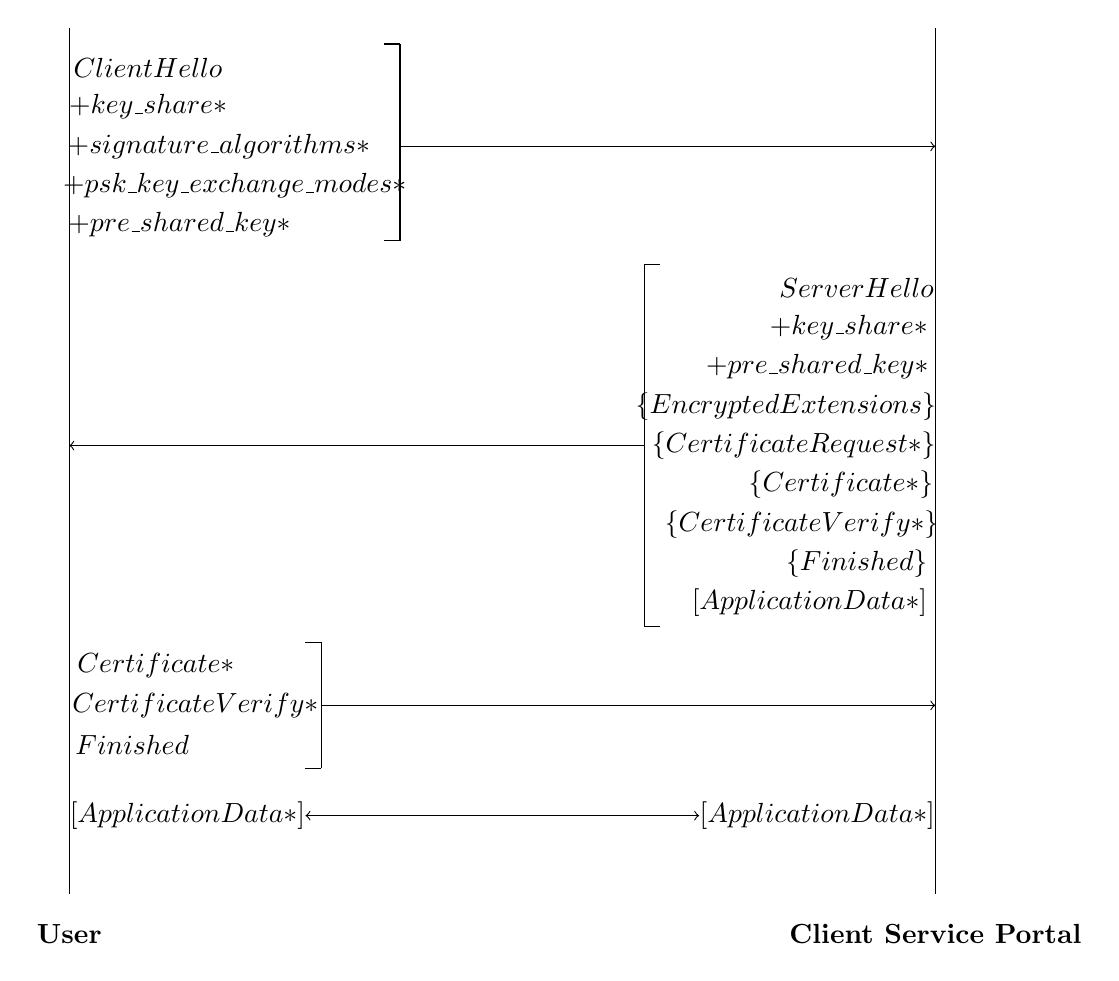
\begin{tikzpicture}

        \node at (-11,-5.5) {$\textbf{User}$}; %0          -1.5
        \node at (0,  -5.5) {$\textbf{Client Service Portal}$}; %0          -1.5

        %client line
        \draw (-11,6) -- (-11,-5);

        %Server line
        \draw (0,6) -- (0,-5);

        %client lessages
        %key exchange
        % \node at (-10,5.5)   {$ClientHello$};

        %---------------------
        \draw (-6.8,5.8) -- (-6.8,3.3);
        \draw (-7,5.8) -- (-6.8,5.8);
        \draw (-7,3.3) -- (-6.8,3.3);
        \node at (-10,5.5)   {$ClientHello$};
        \node at (-10,5)     {$+ key\_share*$};
        \node at (-9.1,4.5)   {$+ signature\_algorithms*$};
        \node at (-8.9,4)     {$+ psk\_key\_exchange\_modes*$};
        \node at (-9.6,3.5)   {$+ pre\_shared\_key*$};
        \draw[->] (-6.8,4.5) -- (0,4.5);


        %Server messages
        \draw (-3.7,   3) -- (-3.7,-1.6);
        \draw (-3.7,   3) -- (-3.5,   3);
        \draw (-3.7,-1.6) -- (-3.5,-1.6);


        \node at (-1,2.7)   {$ServerHello$};
        \node at (-1.1,2.2)   {$+ key\_share*$};
        \node at (-1.5,1.7)   {$+ pre\_shared\_key*$};
        \node at (-1.9,1.2)   {$\{EncryptedExtensions\}$};
        \node at (-1.8,.7)   {$\{CertificateRequest*\}$};
        \node at (-1.2,.2)   {$\{Certificate*\}$};
        \node at (-1.7,-.3)   {$\{CertificateVerify*\}$};
        \node at (-1,-.8)   {$\{Finished\}$};
        \node at (-1.6,-1.3)   {$[Application Data*]$};
        \draw[<-] (-11,.7) -- (-3.7,.7);

        %clent messages
        \draw (-7.8,-1.8) -- (-7.8,-3.4);
        \draw (-8,-3.4) -- (-7.8,-3.4);
        \draw (-8,-1.8) -- (-7.8,-1.8);
        \node at (-9.9,-2.1)   {${Certificate*}$};
        \node at (-9.4,-2.6)     {${CertificateVerify*}$};
        \node at (-10.2,-3.1)   {${Finished}$};
        \draw[->] (-7.8,-2.6) -- (0,-2.6);

        %communication start
        \node at (-9.5,-4)   {$[Application Data*]$};
        \node at (-1.5,-4)   {$[Application Data*]$};
        \draw[<->] (-8,-4) -- (-3,-4);

    \end{tikzpicture}
    \caption{TLS 1.3 Handshake. In the figure $+$ Indicates noteworthy extensions sent in the previously noted message. $*$ Indicates optional or situation-dependent messages/extensions that are not always sent. $\{\}$ Indicates messages protected using keys derived from a [sender]$\_$handshake$\_$traffic$\_$secret. $[]$ Indicates messages protected using keys derived from [sender]$\_$application$\_$traffic$\_$secret$\_N$.}
    \label{TLS1.3_handshake}
\end{figure}
%-------------------------------------------------------------------------------------------------------




\begin{comment}
%Figure to show the TLS1.3 connection istablishment
\begin{figure}[!ht]
    \centering
    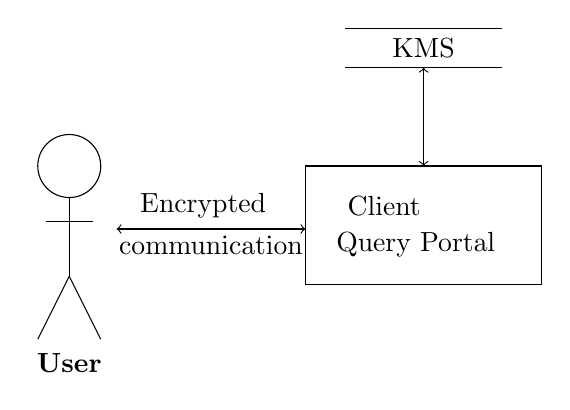
\begin{tikzpicture}

        %Drawing an User
        \draw (-12,0) circle [radius=.4]; %head
        \draw (-12.3,-.7) -- (-11.7,-.7);  %hands .4 -.4   .7 .7
        \draw (-12,-.4) -- (-12,-1.4); %spinal cord  0 0    .4 1.4
        \draw (-12,-1.4) -- (-12.4,-2.2); %left leg 0 .4     1.4 2.2
        \draw (-12,-1.4) -- (-11.6,-2.2); %right leg 0 -.5    1.4  2.2
        \node at (-12,-2.5) {$\textbf{User}$}; %0          -1.5

        % Service Query Portal
        \draw (-9,-1.5) -- (-6,-1.5) -- (-6,0) -- (-9,0) -- (-9,-1.5);
        \node at (-8,-.5) {Client};
        \node at (-7.6,-1) {Query Portal};

        %Database drawing
        \draw (-8.5,1.75) -- (-6.5,1.75);
        \draw (-8.5,1.25) -- (-6.5,1.25);
        \node at (-7.5,1.5) {KMS};

        %connecting arrow between user and client query portal
        \draw [<->](-11.4,-.8) -- (-9,-.8);
        \node at (-10.3,-.5) {Encrypted};
        \node at (-10.2,-1) {communication};

        %Connecting line between KMS and client query portal
        \draw [<->](-7.5,1.25) -- (-7.5,0);

    \end{tikzpicture}
    \caption{Interaction between user and the client query portal}
    \label{fig_user_Client_query_portal_interactions}
\end{figure}
\end{comment}






Once the key materials are shared using TLS $1.3$, all followed interactions are performed using the cryptographic parameters shared during the TLS handshake protocol in the encrypted domain as depicted by figure \ref{fig:basic_dfd}. TLS handshake protocol allows both parties to negotiate a protocol version, select cryptographic algorithms, optionally authenticate each other and establish shared secret keying material. Once handshaking is complete, parties use the specified keys to protect the application-layer data. Failure of the handshake or other protocol triggers termination of the connection, optionally preceded by an alert message.


%and tried to mitigate anomalies observed.
When a client performs secure authentication using his credentials, viz username, and password, he can use the registered services available for the users. However, it is emphasized that the query encryption key is never shared with the user. The user's query is encrypted in the client service portal using the standard methods present in the client service portal. By doing so, use of more errors for query encryption for an intentional decryption failure attack can be safely restricted. Additionally, there needs to be more than encrypted communication between the user and the client service portal to ensure secure query encryption. The user, as well as the client service portal, may be malicious and may act as an active or passive attacker. Thus all possible behavior of the user and client service portal must be analyzed, and its mitigation techniques must be suggested. Below, we have performed a case study on the user and the client service portal based on their behavior.

The user's query can be sent for computation to the query service portal in two different ways. Each of these has its associated advantage and shortcomings. Either of these techniques is implementation specific and decided based on project requirements. In our case, we suggest using the second technique for HE deployment.

In the first technique, a user query is sent with user metadata for query computation. In this case, the user's authentication is performed using the user database stored in the server, and the same is true for the service validity check. After successful authentication and verification, the query computation is performed, which is decrypted and decoded, and the obtained final plain result is forwarded to the user who submitted the query. This method requires maintenance of the user's database on the server side. Similarly, the user's service information must be stored on the server side for a service check. As more users register with the institutions, they must constantly update and maintain the database. Similarly, when a user's registration has been withdrawn, it has to be updated on the server side, which creates a heavy overload on the server side.

In the second technique, the user's query is sent with the institution's metadata. When a user asks for a query request, the user's authentication is verified in the client-side portal. On successful authentication, the user's queries are sent with the institution's metadata storing the user's information requesting the service on the client-side portal, specifically in the service request database. The server side performs institution authentication and service validation of the institution. On successful authentication and service request verification, query computation is performed. The result is forwarded to the institution. The institution identifies the user who generated the query request from the service request database and sends the query result to the corresponding query user.



\newpage

\section{Client Side Security Analysis: Secure communication}
\label{possible-attacks_in_components}

\subsection{User}
\begin{itemize}
    \item An unauthorized user tries to access the services
          \begin{itemize}
              \item To access services the user needs to be registered; upon registration, login credentials are provided to the user.
              \item Unless the user has the login credentials of a registered user, he can not access the services.
              \item Upon registration user gets the signing key that he uses for creating query signature and send with query.
          \end{itemize}

    \item A user uses brute force to guess login credentials of registered user
          \begin{itemize}
              \item These types of attacks can be restricted by using an additional layer of authentication in the form of multifactore authenticator to use the facility.
              \item However, during implementation, it needs to be ensured that the user's credentials are verified only after multifactore authentication.
              \item On successful multifactore authentication, user's credentials are verified a threshold number of times, and after that user may be blocked for a specific time interval based on the security requirements.
          \end{itemize}

    \item An attacker may try to steal the login information of the user by social engineering or by impersonation attack (attempt to gain unauthorized access to systems by masquerading as authorized users)
          \begin{itemize}
              \item As mentioned above, these attacks can be restricted using an additional layer of authentication in the form of multifactore authentication.
          \end{itemize}

    \item Attackers may eavesdrop on the communication link, modify the communicated data or prevent communication between the user and the client service portal
          \begin{itemize}
              \item As mentioned above, the user and client service portal communicates using a secure communication channel built using TLS1.3. Thus eavesdropping on the communication link between the user and the client service portal is restricted by TLS1.3.
          \end{itemize}

    \item User uses feedback mssages to gain secret information about the system
          \begin{itemize}
              \item Feedback messages do not reveal any secret information to the user by design. It will be clear when we discuss the feedback messages sent to the user.
          \end{itemize}
    \item A genuine user forgets his password
          \begin{itemize}
              \item On successful completion of multifactor authentication user is taken to the password reset page where he can reset his password
          \end{itemize}
    \item User revocation by institution
          \begin{itemize}
              \item In such cases, user can not pass the client service portal
              \item This must be easy to implement and operate
          \end{itemize}
\end{itemize}


\subsection{Client Service Portal}

Clent service portal can be further divided into two categories: Compromised and Passive Attacker. Below we will study security threats posses to the system by each of these categories.
\subsubsection{Passive Attacker}
\begin{itemize}
    \item Denial of service attack
          \begin{itemize}
              \item The user cannot perform any query on the database.
              \item The reason is mentioned in the feedback reply sent to the user with the standard error code.
          \end{itemize}
    \item The authorization of an unauthorized user
          \begin{itemize}
              \item This situation may arise when a user is completely compromised.
              \item An attacker with the key and metadata of a genuine user can’t be detected, provided he has access to the multifactor authenticator.
              \item Thus, he can perform query computation without any problem and finally gets the result as a regular genuine user.
              \item However, this type of attack can be avoided by sending a feedback reply to the user on user login. If he is not the one into the system then he is suggested to change his credentials immediately.
          \end{itemize}

    \item Institution revocation by Service Query Portal
          \begin{itemize}
              \item Institution can not perform any query operation
              \item This operation must be easy to implement and operate
          \end{itemize}

\end{itemize}

\subsubsection{Compromised}
\begin{itemize}
    \item Genuine user authentication failure
          \begin{itemize}
              \item The user cannot login to the client service portal the perform query on the database.
              \item However, the user knows why the authentication failed through the feedback received.
              \item The feedback sent has the reason behind the authentication failure as a standard error code like user credentials are incorrect.
          \end{itemize}
    \item The requested service was not provided to the user
          \begin{itemize}
              \item The user cannot perform the intended service computation on the database.
              \item The reason is mentioned with a standard error code in the feedback reply. Thus the user knows the reason behind the requested service failure.
          \end{itemize}

          %         \item Client Service Portal can send (encryption key, metadata) in the following four possible ways
          %
          %             \begin{itemize}
          %                 \item Correct, Correct
          %                 \begin{itemize}
          %                     \item This is correct and creates no problem for query computation
          %                 \end{itemize}
          %                 \item Correct, Wrong
          %                 \begin{itemize}
          %                     \item Wrong here means metadata is of another user
          %                         (If metadata is completely wrong, then it gets detected in the service query portal when user is verified)
          %                     \item The user encrypts his query and sends it for query computation
          %                     \item Service query portal authenticates the user and sends it to FHE Query Engine
          %                     \item Service registry authenticates the user if it has access for the service requested then he replies with the user metadata
          %                     \item The service key is asked from service KMS using user’s metadata and service KMS replies with necessary keys
          %                     \item FHE query engine performs query computation and stores it in the encrypted form
          %                     \item Encrypted result is decrypted in the TEE and later it is sent to the user.
          %                     \item However, the result obtained by the user is wrong due to wrong key used for query encryption in the first place itself.
          %                     \item \textcolor{blue} {I think this form of attack can be restricted by storing metadata and key along with its DS}.
          %                 \end{itemize}
          %                 \item Wrong , Correct
          %                 \begin{itemize}
          %                     \item Using the same techniques as that of above this form of attack can be identified and restricted
          %                 \end{itemize}
          %                 \item Wrong, Wrong
          %                 \begin{itemize}
          %                     \item He gets detected in the service query portal when the user gets verified
          %                 \end{itemize}
          %             \end{itemize}


    \item The query malleability
          \begin{itemize}
              \item Query encryptions are performed in three steps in the order: encoding, encryption, and signature computation.
              \item Query encryption is performed in the TEE environment in the client service portal.
              \item Before query encryption query malleability check is performed inside the TEE environment. On successful query signature validation, query encoding is performed, followed by query encryption.
              \item Query signature computation is performed upon query encryption.
              \item Finally, the obtained encrypted query and query signature is sent to Service Query Portal for query computations.
              \item Query malleability on transit can be restricted by using TLS1.3 by creating a secure communication channel.+6
          \end{itemize}
\end{itemize}


\section{Server Side Security Analysis: HE Computation}

In the second part security of homomorphic computation is taken care of. In this part, all communication performed by the client query portal having encrypted query to obtain a query answer and homomorphic computation is handled. In the process, if any entity leaks any sensitive information, it is analyzed, and mitigation techniques are suggested to avoid such attacks or leakages. For completeness of risk analysis, we will consider each entity individually, considering what information is available to the entity and, using that, what kind of security threat the entity may pose to the system if the entity behaves as a passive or as an active attacker. We will also consider what kind of secret information the system may leak as a whole and by each entity during HE computation and try to suggest technologies that can be used to avoid such leakages.


%----------------------------------------------------
\label{possible-attacks_in_components}

\subsection{Service Query Portal}
\begin{itemize}
    \item Denial of service attack
          \begin{itemize}
              \item Institution cannot perform any query on the database
              \item However, this can be avoided using standard techniques of overcoming denial of service attack
          \end{itemize}
    \item Authorization failure attack
          \begin{itemize}
              \item The institution cannot perform any query on the database
              \item However, the same is conveyed to the institution by a standard error code as a feedback message sent.
          \end{itemize}
    \item Query malleability attack
          \begin{itemize}
              \item The query service portal can perform query malleability
              \item However, this can be avoided by sending digital signature of the encrypted query along with the query.
          \end{itemize}
    \item Query id malleability attack
          \begin{itemize}
              \item If the query id is modified, then it produces results, but the genuine user can’t fetch the result in the final step.
              \item However, this can be restricted by including the Institutional id, user id, and job id in the digital signature computation by the client service portal.
              \item Thus, by checking the digital signature, the query is dropped with a standard message sent back to the user if any discrepancy is found.
          \end{itemize}
    \item Incorrect digital signature received from the client query portal
          \begin{itemize}
              \item Service query portal discards the query if digital signature check fails
              \item Sends feedback to the user with a standard error message representing digital signature check fail.
          \end{itemize}
\end{itemize}
\subsection{Service Registry}
\begin{itemize}
    \item Denial of service attack
          \begin{itemize}
              \item Institution are not allowed to perform any query on the database
              \item This can be avoided by using standard techniques of overcoming denial of service attacks
          \end{itemize}
    \item Service authentication fail
          \begin{itemize}
              \item Query discarded from further processing
              \item However, the institution is informed by sending feedback message with standard error code representing service authentication fail
          \end{itemize}
    \item Service registry sends incorrect user metadata (Service Id, Service Name, HE Parameters, HE Client)
          \begin{itemize}
              \item This kind of discrepancies can be avoided by storing digital signature computed as DS(Institution Id + Service Id + Service name + HE Parameters + HE Client)
              \item Thus, when TEE gets the service parameters (Service Id, Service Name, HE Parameters, HE Client) from Service Registry and query information (Institution Id + Service Id + Service name) from query metadata. It computed the signature and verifies that it has indeed received the correct service parameters.
              \item If the computed DS do not match with that of the obtained DS, then he can perform either of the following two operation
                    \begin{itemize}
                        \item He can either ask for service parameters from service registry or
                        \item He can send feedback to the institution a stand error code representing service parameter check fail
                    \end{itemize}
          \end{itemize}
\end{itemize}

\subsection{Service Key Management System}
\begin{itemize}
    \item Denial of service attack
          \begin{itemize}
              \item Query processing not allowed to perform on the database
              \item This can be avoided using standard techniques of overcoming denial of service attack
          \end{itemize}
    \item Key malleability attack
          \begin{itemize}
              \item This can be avoided by storing Public key and Evaluation key encrypted with HSM using symmetric key encryption like AES with its digital signature.
              \item Digital signature here is computed as DS(Institution Id + HSM(Public Key) + HSM(Evaluation Key))
              \item TEE performs DS check if any inconsistency is observed
                    \begin{itemize}
                        \item It either requests the service key from service key management system or
                        \item Sends feedback to the institution with standard error code.
                    \end{itemize}
          \end{itemize}
    \item Wrong key Sent
          \begin{itemize}
              \item As mentioned above, the digital signature can be used to check whether the service key management system has sent the wrong key. If so, then appropriate action is taken.
          \end{itemize}
\end{itemize}

\subsection{Database}
\begin{itemize}
    \item Denial of service attack
          \begin{itemize}
              \item Query processing not allowed to perform on the database
              \item This can be avoided by using standard techniques of overcoming denial of service attack
          \end{itemize}
    \item Decryption failure due to wrong data provided for computation
          \begin{itemize}
              \item This type of attacks can be avoided by encrypting database using the attestation key of TEE.
          \end{itemize}
\end{itemize}

\subsection{FHE Query Computation}
\begin{itemize}
    \item Denial of service attack
          \begin{itemize}
              \item Query processing not allowed to perform on the database
              \item This can be avoided by using standard techniques of overcoming DOS
          \end{itemize}
    \item Decryption failure attack due to different circuit computation
          \begin{itemize}
              \item Query is feed along with its digital signature to the TEE
              \item TEE computes digital signature of the query and checks to find out correct circuit has been provided for the computation
              \item If incorrect circuit has been provided for computation, then sends feedback to the user with standard error message.
              \item Thus, this type of attack can be avoided by computing and verifying digital signature inside TEE
          \end{itemize}
    \item Query result malleability attack
          \begin{itemize}
              \item FHE Query Engine can modify the query result
              \item However, this can be restricted by computing query result digital signature in the TEE itself before providing it to FHE Query Engine.
              \item Send both encrypted query result and signature to the encrypted result store
          \end{itemize}
    \item Side channel attack
          \begin{itemize}
              \item Side channel attack can be avoided by computing query result in the TEE
          \end{itemize}
    \item Known plaintext attack (computation performed in plaintext domain)
          \begin{itemize}
              \item  Same as that of the above i.e., computation performed in the TEE
          \end{itemize}
\end{itemize}

\subsection{Decryption and Decoding}
\begin{itemize}
    \item Denial of service attack
          \begin{itemize}
              \item User denied from fetching query result.
              \item However, this can be avoided using standard techniques of overcoming DOS
          \end{itemize}
    \item Query result malleability attack
          \begin{itemize}
              \item TEE before decryption computes signature and checks its integrity with that of the signature received from the FHE Query Engine
              \item If case of any discrepancy, send feedback to the query service portal stating query integrity breached
          \end{itemize}
    \item Decryption failure attack
          \begin{itemize}
              \item If decryption fail is obtained, then it must be genuine and, in such scenario, the obtained result is sent to the User.
          \end{itemize}
    \item Side channel attack
          \begin{itemize}
              \item Decryption of the encrypted query result is performed in the TEE thus avoiding the side channel attack
              \item Also, TEE directly send the decrypted query result to user using HTTPS connection avoiding further attacks while query result is in transit.
          \end{itemize}
\end{itemize}


 % HE deploymet details


% !TeX root = ../sameplaper.tex
% !TeX spellcheck = en_US

\chapter{Homomorphic Encryption}
\setcounter{section}{0}


\section{Security Notion}
We will briefly introduce security notions of cryptography that readers come across when studying homomorphic encryption schemes. Security notions of homomorphic encryption schemes are the same as that of symmetric and asymmetric cryptographic encryption schemes. We briefly review security notions here for a thorough security notion of cryptography; we refer readers to \cite{katz2020introduction}.


\subsection{Security Model}
The notion of an adversary in cryptography is a modeled one. The actual adversaries in the real world are referred to as an attacker. In cryptography, attackers are usually assumed to be computationally bounded and run in probabilistic polynomial time. However, in some cases, computationally unbounded adversaries are also considered. An adversary can corrupt parties involved in the protocol. Based on how parties are corrupted or behave while executing a protocol, adversaries can be classified into Honest-But-Curious (HBC) and Malicious adversaries. The difference between the two adversary models will be clear from the definition below.

\begin{definition} \cite{goldreich2009foundations} (Honest-But-Curious Adversary). An honest-but-curious (HBC) adversary is a legitimate participant in a communication protocol who will not deviate from the defined protocol but can gather all information shared for protocol execution from the legitimately received messages.
\end{definition}

The HBC adversary model is a reasonably weak adversarial model. Still, this model is sufficient to ensure no unintended information leakage from the protocol. Chosen plaintext attack (CPA) is an example of an HBC adversary where the adversary can observe the honestly generated ciphertexts. An HBC adversary model is also known as a semi-honest adversary or passive adversary.


\begin{definition} \cite{goldreich2009foundations} (Malicious Adversary). A malicious adversary is a legitimate participant in a communication protocol who takes active steps to disrupt the execution of the protocol (send messages that differs from those specified by the protocol), or can gather legitimate messages shared for protocol execution (he can use it later or shared with the other dishonest parties).
\end{definition}

A malicious adversary model is a strong adversary model. Chosen ciphertext attack (CCA) is an example of a malicious adversary model where the adversary can ask for any ciphertext of its choice regardless of valid or invalid. Malicious adversaries are also known as an active adversaries.


\subsection{Semantic Security}
Correctly defining security of a protocol or an encryption scheme is non-trivial task. The idea is that the adversary should not learn any partial information about the plaintext from the ciphertext. It is usually formalized using semantic security. Loosely speaking, semantic security means whatever can be efficiently computed from the ciphertext can be efficiently computed given only the length of the plaintext. Note that semantic security does not rule out the possibility of inferring the length of the plaintext from the ciphertext. However other than the length of the plaintext the ciphertext should not yield anything about the plaintext.

Semantic security is complex and difficult to work with. Thus an equivalent definition called \textit{indistinguishability} is used. To be precise an encryption scheme is said to be semantically secure if and only if it has indistinguishable encryptions \cite{goldreich2009foundations}. Below we will briefly review indistinguishability.


\subsection{Indistinguishability}
Indistinguishability is based on an experiment involving an adversary passively observing a ciphertext and then trying to guess the encrypted message. It can be played as a game where an adversary $\mathcal{A}$ first samples two messages $\mu_1$ and $\mu_2$ and sends them to the challenger. The challenger selects one of the message $\mu_1$ or $\mu_2$ with equal probability and encrypts and sends the encrypted message to the adversary. If $\mathcal{A}$ outputs a ``guess" as to which of the two messages was encrypted; $\mathcal{A}$ succeeds if the guess is correct. There are standard models of indistinguishability available for different attack scenarios as defined below.
% INDistinguishability under Chosen Plaintext Attack (IND-CPA), INDistinguishability under Chosen Cihpertext Attack (IND-CCA), INDistinguishability under adaptively Chosen Cihertext Attack (IND-CCA2), INDistinguishability under Cihpertext Verification Attack (IND-CVA) etc as defined below.

\subsubsection{IND-CPA} An encryption scheme is considered IND-CPA secure if no adversary can distinguish encryption of two messages $\mu_1$ and $\mu_2$ better than probability $\frac{1}{2}$. Here the adversary has black-box access to an encryption oracle, and he can ask for encryption of the plaintext message of his choice. The idea of this security definition is that even if the adversary has access to the encryption oracle, he can not deduce any information about the plaintext by simply observing ciphertext.

IND-CPA is equivalent to the property of semantic security, and many cryptographic proofs use these definitions interchangeably. It is the standard security requirement for an encryption scheme. State-of-the-art homomorphic encryption schemes, regardless of whether integers-based or LWE-based, provides IND-CPA security by direct reduction to an intractable problem.

Notice that any scheme that achieves IND-CPA security is secure in the presence of an HBC adversary. Also, by this security definition, any deterministic encryption scheme cannot be secure as the adversary can ask for encryption of messages $\mu_1$ and $\mu_2$, compare it with the challenge ciphertext and produce the result with probability 1.

\subsubsection{IND-CCA} An encryption scheme is said to be IND-CCA secure if no adversary can distinguish encryption of two messages $\mu_1$ and $\mu_2$ better than $\frac{1}{2}$ probability even if the adversary has black-box access to the encryption and decryption oracle before the challenge ciphertext $c$ is published. Alternatively, the adversary should not learn any information about the plaintext message by looking into the ciphertext even after having black-box access to the encryption and decryption oracle. IND-CCA is a stronger security notion than IND-CPA.

It has been shown in \cite{loftus2011cca,zhang2012cca,chenal2015key} that almost all somewhat homomorphic encryption schemes proposed till now are vulnerable to non-adaptative chosen ciphertext attacks (CCA1), revealing the decryption key. In fact it is obvious that no malleable encryption scheme can achieve full IND-CCA security. More discussion about the same can be obtained in \cite{bellare1999non}.

In general, all somewhat homomorphic encryption schemes based on LWE or its ring variant, and also those based on integers, rely on a search-to-decision reduction. This basically means that being able to decrypt a homomorphic ciphertext is equivalent to recovering the private key, which itself reduces to solving some intractable problem in the worst case. Suppose this feature allows elegant IND-CPA security proofs. In that case, it also means that any (CCA1) decryption oracle breaks the scheme just by following the steps of the search-to-decision reduction.




\subsubsection{IND-CCA2} IND-CCA2 security is a stronger security notion than that of IND-CPA and IND-CCA. An encryption scheme is said to be IND-CCA2  secure if no adversary can distinguish encryption of two messages $\mu_1$ and $\mu_2$ better than $\frac{1}{2}$ probability, even if he has black-box access to the encryption and decryption oracle even after obtaining a challenge ciphertext $c$ except that he can not ask for decryption of the challenge ciphertext $c$.

No homomorphic primitive can be IND-CCA2 secure since their main feature is to be malleable.

\subsubsection{IND-CVA}Standard security definition alone may not be sufficient when we study encryption schemes from a deployment point of view. We must see beyond the encryption primitive and consider a broader view of the overall system deployement. In case of homomorphic encryption following questions makes sense when considered deployment.
\begin{enumerate}
    \item Can the cloud have some meaningful information when it behaves as an active attacker ? or
    \item Can a user acting as a passive or an active attacker can perform some attacks when it gets access to the decryption oracle?
\end{enumerate}



In some encryption schemes, extracting the secret key itself might be possible if the attacker gets access to the decryption oracle like the one presented by Li et al. \cite{li2021security} in the case of approximate encryption scheme \cite{cheon2017homomorphic}. This was possible due to secret key leakage in the decrypted ciphertext. However, these types of attacks are not possible in the exact homomorphic encryption scheme. Still, we need to consider possible attack scenarios when deploying a homomorphic encryption scheme for real-world applications.

Indistinguishability under Ciphertext Verification Attacks (IND-CVA) allows the adversary to access to both encryption oracle and ciphertext verification oracle. This notion of security is slightly stronger than IND-CPA but much weaker than IND-CCA \cite{hu2009ciphertext}.
% It many be used to attack the deployment scenario by modifying few bits of the ciphertext and observing the clients behaviour.
% \paragraph{Safe-error and reaction attack}: The security of homomorphic encryption primitive are not sufficient to use homomorphic encryption schemes in real-world applications. It must be studied by considering the broader view or construction of how the schemes have been used for the application.
IND-CVA focus on the overall deployment or system behavior. These are the attacks that are performed by an active attacker. This type of attack is feasible when the cloud behaves as an active attacker. These attacks focus on and use the overall deployment behavior when a small error is injected into the computed result. The devastating nature of this type of attack has been studied in \cite{chillotti2016attacking} and suggested some technique to avoid such attacks viz.

The mitigation techniques of such attacks is to use signatures along with the encrypted data. Compute and check signatures before processing the data for its integrity.



\section{FHE Security Assumption} Deployment of encryption schemes for real-world applications needs some standards and security parameterization. The same goes for homomorphic encryption schemes. Standards of homomorphic encryption have been studied and presented in the report \cite{albrecht2021homomorphic}. The report presents the currently known state-of-the-art lattice attacks on lattice-based encryption schemes and recommends a wide selection of parameters to be used for homomorphic encryption for various security levels. The report also describes the additional features of HE schemes which make them useful in different application scenarios.

Below we have briefly reviewed hard problems backing homomorphic encryption schemes followed by known attacks and their computation complexity.

\subsection{Hard problems}
In the literature to design homomorphic encryption schemes, different hard problems have been used, viz. NTRU ($N^{th}$ degree Truncated polynomial Ring Units) problem, AGCD (Approximate Greatest Common Divisor) problem, LWE (Learning With Error) problem and it's variant R-LWE (Ring Learning With Error) problem. However, not all these hard problems give rise to equally efficient encryption schemes. LWE and R-LWE-backed encryption schemes are usually more efficient from practical considerations. They produce comparatively smaller size ciphertext than the others. However, encryption schemes backed by an overstretched \cite{albrecht2016subfield} variant of the NTRU computational problem are shown to be vulnerable to subfield lattice attacks \cite{albrecht2016subfield,cheon2016algorithm}; thus, they are no longer used in practice. For the same reason, we will not introduce NTRU problem here.


\subsubsection{Learning With Error (LWE) Problem}
Introduced by Regev \cite{regev2009lattices}, learning with errors (LWE) problem finds many application in cryptography. The LWE problem can be defined as follows.

\begin{definition}For security parameter $\lambda$, let $n = n(\lambda)$ be an integer dimension, let $q = q(\lambda) \geq 2$ be an integer modulus, and let $\chi = \chi(\lambda)$ be an error distribution over $Z$. The decisional version of $LWE_{n,q,\chi}$ problem is to distinguish the following two distributions:

    In the first distribution, one samples $(a_i, b_i)$ uniformly from $Z^{n+1}_q$.

    In the second distribution, one first draws $s \leftarrow Z^n_q$ uniformly and then samples $(a_i, b_i) \in Z^{n+1}_q$ by sampling $a_i \leftarrow Z^n_q$ uniformly, $e_i \leftarrow \chi$, and setting $b_i = <a_i,s> + e_i$.

    The search version of the $LWE_{n,q,\chi}$ problem corresponds to the recovery of the secret vector $s$ given polynomially many samples from the second distribution.

    The $LWE_{n,q,\chi}$ assumption is that the $LWE_{n,q,\chi}$ problem is infeasible.
\end{definition}

The error distribution $\chi$ can be either a discrete Gaussian distribution over the integers, a continuous Gaussian distribution rounded to the nearest integer, or other distributions supporting small integers.

Security of the LWE problem is established by quantum reduction from hard lattice problems such as GapSVP and SIVP \cite{regev2009lattices}. %$An efficient solution to the LWE problem implies a quantum algorithm for GAPSVP and SIVP.
In fact, for the hardness of LWE problem when the error distribution $\chi = \mathcal{D}_{Z,\alpha q}$ where $\alpha \cdot q \geq 2 \sqrt{n}$, it has been established that the search version of LWE is at least as hard as quantumly approximating certain worst-case problems on $n$-dimensional lattices to within $\tilde{O}(n/\alpha)$ factors \cite{regev2009lattices}. Moreover, for similar parameters and large enough $q$, search-LWE is at least as hard as classically approximating the decision shortest vector problem and variants \cite{peikert2009public}. For moduli $q$ that are sufficiently `smooth' (i.e., products of small primes), the decision form of LWE is at least as hard as the search form \cite{peikert2009public,regev2009lattices}. It has been also established that the decision-LWE remains hard even if the secret $s$ is chosen from the error distribution $\chi$, rather than uniformly at random \cite{micciancio2009lattice,applebaum2009fast}.  Although, binary, and ternary LWE is easier than general LWE still properly choosen parameters can provide binary-LWE same securty as that of the standard LWE problem \cite{chen2020concrete,bai2014lattice}.



\subsubsection{Ring Learning With Error (R-LWE) Problem}

Introduced by Lyubaskevsky, Peikert and Regev \cite{lyubashevsky2013ideal} the ring learning with errors (R-LWE) problem finds many applications in cryptography. Here we provide a simplified special-case version of the problem that is easier to understand and work with \cite{brakerski2011fully},\cite{regev2010learning}.

\begin{definition}
    For security parameter $\lambda$, let $f(x) = x^d+1$ where degree $d = d(\lambda)$ is a power of 2. Let modulus $q = q(\lambda) \geq 2$ be an integer. Let $R = Z[x]/(f(x))$ and let $R_q = R/qR$. Let $\chi = \chi(\lambda)$ be a distribution over $R$. The decisional R-LWE$_{d,q,\chi}$ problem is to distinguish the following two distributions:

    In the first distribution, one samples $(a_i, b_i)$ uniformly from $R^2_q$.

    In the second distribution, one first draws secret $s \leftarrow R_q$ uniformly and then samples $(a_i, b_i) \in R^2_q$ by sampling $a_i \leftarrow R_q$ uniformly, $e_i \leftarrow \chi$, and sets $b_i = <a_i, s> + e_i$.

    The search version of the R-LWE$_{n,q,\chi}$ problem corresponds to the recovery of the secret $s$ given polynomially many samples from the second distribution.

    The R-LWE$_{d,q,\chi}$ assumption is that the R-LWE$_{d,q,\chi}$ problem is infeasible.
\end{definition}

The efficiency of the R-LWE problem over LWE problem is that though in R-LWE each noisy product $b \approx a\cdot s$ gives $n$ simultaneously pseudorandom values over $\mathbb{Z}_q$ unlike LWE, still the cost of generating it is significantly small. In general polynomial multiplication can be performed in $O(n\log{n})$ scalar operations and in parallel depth $O(\log{n})$, using  Fast Fourier Transform (FFT) or its variants. Also, in most applications, $(a,b)\in R_q \times R_q$ from the R-LWE distribution can replace $n$ samples $(\textbf{a},b)\in \mathbb{Z}_q^n\times \mathbb{Z}_q$ from the standard LWE distribution; reducing the public key size by a factor of $n$. This dramatically reduces the public key size of homomorphic encryption schemes.

Security of the R-LWE problem is established by quantum reduction from the approximate Shortest Vector Problem (SVP) (in the worst case) on ideal lattices in $R$ to the search version of the R-LWE problem.

\subsubsection{Approximate Greatest Common Divisor (AGCD) problem} Introduced by Howgrave-Graham in \cite{howgrave2001approximate}, AGCD is an alternative way of designing homomorphic encryption schemes. The problem can be defined as %The first alternative design was proposed by van Dijk, Gentry, Halevi and Vaikuntanathan \cite{van2010fully} in 2011. The AGCD problem can be defined as
\begin{definition}
    Let $\rho,\eta,\gamma$ and $p$ be integers such that $\gamma > \eta > \rho > 0$ and $p$ is an $\eta$-bit prime number. The distribution $D_{\gamma,\rho}(p)$, whose support is $[0, 2^{\gamma}-1]$ is defined as
    \begin{align*}
        D_{\gamma,\rho}(p) & := \{Sample\ q \leftarrow [0, 2^{\gamma}/p[ \ and\ r \leftarrow ]-2^{\rho},2^{\rho}\ [\ Output\ x := pq + r\}
    \end{align*}
    The ($\rho, \eta, \gamma$)-AGCD problem is the problem of finding $p$, given polynomially many samples from $D_{\gamma,\rho}(p)$.

    The ($\rho,\eta,\gamma$)-decisional-AGCD problem is the problem of distinguishing between $D_{\gamma,\rho}(p)$ and $\mathcal{U}([0, 2^{\gamma}[)$.
\end{definition}

AGCD problem is believed to be hard even in the presence of quantum computers. In fact, when the parameters ($\rho,\eta,\gamma$) are chosen properly, the best known attacks against it run in exponential time \cite{galbraith2016algorithms}. Moreover, when $p,q_i$ and $r_i$ are sampled from a specific distributions, then the AGCD problem becomes at least as hard as the LWE problem \cite{cheon2015fully}.

The first homomorphic encryption scheme over the integers designed using the hardness of the AGCD problem was proposed by Dijk et al. \cite{van2010fully} in 2010. The original work is followed by the subsequent work few of which includes \cite{cheon2013batch,coron2014scale,cheon2015fully,benarroch2017fhe,pereira2020efficient} to name a few, however, the list goes on. Each of these works tried to improve the performance of a homomorphic encryption scheme designed using the AGCD problem.



\subsubsection{NTRU Problem}
Introduced by Hoffstein, Pipher, and Silverman \cite{NTRUJHJPJHS,NTRUEncrypt,hoffstein2006ntru} in 1996, NTRU is an efficient lattice based encryption scheme. The problem is be defined as
\begin{definition}
    Let $q \geq 2$ an integer and $\gamma > 0$ a real number. A $(\gamma, q)$-NTRU instance is an element $h \in R_q=\mathbb{Z}_q[x]/(x^d+1)$(ring of integers of the degree-$d$ cyclotomic number field) such that there exists $(f,g) \in R^2 \setminus \{(0,0)\}$ with $g\cdot h = f \ mod\ q$ and $||f||,||g|| \leq \sqrt{q}/\gamma$. The pair
    $(f,g)$ is called a trapdoor of the NTRU instance $h$.

    For $t \geq 1$ and $\gamma$ and $q$ as above, a $(\gamma,q,t)$-tuple-NTRU instance is a tuple $(h_i)_{i\leq t} \in R_q$ such that there exists $((f_i)_{i\leq t},g) \in R^{t+1} \setminus \{(0,\cdots,0)\}$ with $g\cdot h_i=f_i$ mod $q$ and $max_i ||f_i||,||g|| \leq \sqrt{q}/\gamma$.


    % \begin{definition}
    % Let $q \geq 2$, $\gamma > 0$ and $D$ a distribution over $(\gamma, q)$-NTRU instances. A $(D, \gamma, q)$-NTRU probabilistic polynomial time algorithm (with respect to $\log{q}$ and $\log{\Delta_K}$) sampling triples $(h, f, g) \in R_q \times R^2$ such that
    % \begin{itemize}
    %     \item The marginal distribution of $h$ is $D$,
    %     \item $(f,g) \ne (0,0)$ and $||f||,||g||\leq \sqrt{q}/\gamma$,
    %     \item $g\cdot h= f \mod q$
    % \end{itemize}
    % \end{definition}

    For a  distribution $D$ over $(\gamma, q)$-NTRU instances. The $(D, \gamma, q)$ decisional NTRU problem ($(D, \gamma, q)$-dNTRU for short) is the problem of distinguishing  between the samples from $D$ and from $U(R_q)$.

    The $(D, \gamma, \gamma',q)$ $(\gamma \geq \gamma' > 0)$ search NTRU problem is the problem of computing a pair $(f,g) \in R^2 \setminus \{(0,0)\}$ such that $g \cdot h = f\ mod\ q$ and $||f||, ||g|| \leq \sqrt{q}/\gamma'$ given an input $h$ sampled from $\mathcal{D}$.

\end{definition}

Note that any $(\gamma, q)$-NTRU instance is also a $(\gamma',q)$-NTRU instance for any $\gamma'\leq\gamma$.



Initially, the NTRU problem lacked security proof. In 2011, Stehl\'{e} and Steinfeld \cite{stehle2011making} showed how to modify NTRU to reduce security to standard problems in ideal lattices. In 2012, LTV \cite{lopez2012fly} proposed a fully homomorphic encryption scheme based on NTRU using overstretched \cite{albrecht2016subfield}(when $q$ is super-polynomial in $d$) variant of the NTRU problem. The work of BLLN \cite{bos2013improved} follows the work of LTV with a more enhanced encryption scheme.

Recently, Albrecht et al. \cite{albrecht2016subfield} showed that overstretched NTRU is vulnerable to subfield lattice attacks, and it is believed to be over of NTRU-based homomorphic encryption schemes. Later, it was defined precisely how much is called overstretched in NTRU by Ducas et al. \cite{ducas2021ntru,bonte2023final}. Thus security of NTRU-based homomorphic encryption can be established by properly selecting parameters restricting it from overstretching.



\section{HE Parameterization}
The security of a homomorphic encryption scheme depends on the underline hard problems and their parameters. The hardness of homomorphic encryption schemes is based on the hardness of LWE or a Ring-LWE problem. Thus security of the HE scheme is defined using a ring $R$ with dimension $n$, ciphertext modulus $q$, error distribution $\chi$, and a choice of secret distribution $s$.
\subsection{Ring} : Ring $R$ to use in a homomorphic encryption scheme is a power of $2$-cyclotomic polynomial as $R=Z[x]/(x^n+1)$, where $n$ is a power of $2$. For these rings, no known attacks are available that work better than attacks on the LWE problem.

\subsection{Error distribution} In homomorphic encryprion error is usually sampled from Discrete Gaussian distribution with standard deviation $\sigma$=$\frac{8}{\sqrt{2\pi}}$. The reason behind the use of Discrete Gaussian distribution is motivated by the theoretical security reduction provided by \cite{lyubashevsky2013ideal}.However, those theoretical guarantees do not apply to fixed small error widths such as $\sigma$=$\frac{8}{\sqrt{2\pi}}$, and would instead require that the error width grow with the square root of the dimension of the lattice, $\sqrt{n}$ . None of the known attacks appear to take advantage of the shape of the error distribution, only the width; however, the analysis of the security levels given below relies on running time estimates which assume that the shape of the error distribution is Discrete Gaussian. For that reason we continue to assume that the error is chosen from a Discrete Gaussian distribution of fixed small width. The width is chosen to be small for practical performance reasons, and is justified by the concrete running times of known attacks with those error widths. However, over time if attacks improve or new attacks are found, the width of the error may need to be increased in practice.

\subsection{Secret key distribution} For efficiency reasons, in practice we often choose the secret from a non-uniform distribution, such as the ternary distribution, which means to select uniformly from $\{-1,0,1\}$. In the recommended parameters given below, we will present tables for three choices of secret-distribution:{uniform, error, and ternary}. We will not present tables for sparse secrets because we do not suggest standardizing the case of sparse secret due to significantly better known attacks.


\subsection{Recommended parameters for HE}
Table \ref{Tab:parameters_HE} shows the list of parameter values suggested by the homomorphic encryption standar to retain
different security levels.


\begin{table}[ht]
    \centering
    \begin{tabular}{|c|c|c|c|c|c|}
        \hline
        N                        & security level & $\log q$ & uSVP  & dec   & dual  \\
        \hline
        \multirow{3}{4em}{1024}  & 128            & 25       & 132.6 & 165.5 & 142.3 \\
                                 & 192            & 17       & 199.9 & 284.1 & 222.2 \\
                                 & 256            & 13       & 262.6 & 423.1 & 296.6 \\
        \hline
        \multirow{3}{4em}{2048}  & 128            & 51       & 128.6 & 144.3 & 133.4 \\
                                 & 192            & 35       & 193.5 & 231.9 & 205.2 \\
                                 & 256            & 27       & 257.1 & 327.8 & 274.4 \\
        \hline
        \multirow{3}{4em}{4096}  & 128            & 101      & 129.6 & 137.4 & 131.5 \\
                                 & 192            & 70       & 193.7 & 213.6 & 198.8 \\
                                 & 256            & 54       & 259.7 & 295.2 & 270.6 \\
        \hline
        \multirow{3}{4em}{8192}  & 128            & 202      & 129.8 & 130.7 & 128.0 \\
                                 & 192            & 141      & 192.9 & 202.5 & 196.1 \\
                                 & 256            & 109      & 258.3 & 276.6 & 263.1 \\
        \hline
        \multirow{3}{4em}{16384} & 128            & 411      & 128.2 & 129.5 & 129.0 \\
                                 & 192            & 284      & 192.0 & 196.8 & 193.7 \\
                                 & 256            & 220      & 257.2 & 265.8 & 260.7 \\
        \hline
        \multirow{3}{4em}{32768} & 128            & 827      & 128.1 & 128.7 & 128.4 \\
                                 & 192            & 571      & 192.0 & 194.1 & 193.1 \\
                                 & 256            & 443      & 256.1 & 260.4 & 260.4 \\
        \hline
    \end{tabular}
    \caption{The differnt parameters shown in the table represents the following: $N$ is the ring dimension, security level is the bit security provided by the parameters equivalent to that of AES bit security. $\log q$ is the number of bits in the modulus $q$. $uSVP$ represents the bit security against unique shortest vector attack, $dec$ represents the bit security against decoding attack and $dual$ represnts the bit security against dual attack.}
    \label{Tab:parameters_HE}
\end{table}



\section{Library}
There are several research groups working around the world in this new technology and have implemented the general-purpose homomorphic encryption schemes mentioned above in the form of  libraries for applications and general-purpose use. Few of these library are shown in Table \ref{Tab:Crypt_library}. One thing that is common in these general-purpose libraries is that are based on the ring learning-with-error (RLWE) problem, and many of them displayed common choices for the underlying rings, error distributions, and other parameters.

\begin{table}
    \begin{tabular}{ |p{2.5cm}||p{3.5cm}|p{3cm}|p{3cm}|}
        \hline
        Library          & Deveploper        & Developed In & Implements \\
        \hline
        Concrete \cite{} & ZAMA              & Rust         & AFG        \\
        CuFHE    \cite{} & AX                & 1            & ALA        \\
        HEAAN    \cite{} & DZ                & 1            & DZA        \\
        HElib    \cite{} & AL                & 1            & ALB        \\
        Lattigo  \cite{} & AS                & 1            & ASM        \\
        NFLlib   \cite{} & AO                & 1            & AGO        \\
        OpenFHE  \cite{} & formerly PALISADE & 1            & 2          \\
        PALISADE \cite{} & AO                & 1            & AGO        \\
        SEAL     \cite{} & AD                & 1            & AND        \\
        TFHE     \cite{} & AO                & 1            & AGO        \\
        \hline
    \end{tabular}
    \caption{Table showing the HE libraries available}
    \label{Tab:Crypt_library}
\end{table}




 %Details on Homomorphic encryption


% !TeX root = ../sameplaper.tex
% !TeX spellcheck = en_US

\chapter{HE Key Management}
\setcounter{section}{0}

\section{Key Management System}

Recommendation for key management compiled by NIST \cite{KMSV5},\cite{KMS} provides cryptographic key-management guidance. In our scenario, we can use the recommendations they mentioned for HE key management for the smooth management of HE keys. In our deployment, we assume that encryption keys are generated by \textcolor{red}{Database owner} as he is the sole owner of the database and wants to ensure that his database's privacy never gets breached. However, he can hire a third party for the key generation. The third-party generates the HE keys based on the required security level, which the KMS later manages.

The KMS is the one responsible for management of FHE keys stored. These keys are later requested by Client Service Portal and TEE computing the decryption and decoding operations. Keys stored in the KMS have to provide security from all forms of attackers. Here are some guidlince to store keys for overall secure FHE query computation.

\begin{enumerate}
    \item If same public key is used for all users in the institution then encryption key must be the private key corresponding to the public key of the same institution. If this is the case then all institution must have the same public key. If different public key has been used for different institutions then what encryption key or private key has been used to encrypt the data?

    \item Is it that different public key has been generated for the same private keys?

    \item If so what will be its effect viz. how many public keys we can generate without revealing or leaking any information about the private key to the Query service portal behaving as an active attacker?
\end{enumerate}





\newpage
\section{Questions}
\begin{enumerate}
    \item What happens when the homomorphic encryption keys are compromized? written below
    \item Attack to the HE system -------- User adds more errors to the query for decryption failure, corrupted cipher text, corrupted result, effective ways of communication, encoding is known to the attacker.
          ----- Quantify the risk for all the above possibilities? Not necessary to address may come from the protocol itself
    \item How the system behaves when one entity crashes? No side informations leak
    \item Effect of behaviour of one component to the next component when they are in pipeline? By design it will stop working
          \textcolor{blue} {\item What happens when more than one entity comes together to perform an attack?}
    \item How to avoid Service Query Portal performing active attack say changes the digital signature of the user by its own signature? \textcolor{blue} {Can he perform such attack? May be restricted using centralized key storage}
          \textcolor{blue} {\item What will be the overhead of using TEE in the cloud computation as mentioned above in the encrypted cloud computation? Present in literature mentioned in ETH paper
    \item What information is leaked by the feedback system? Done
    \item Can a genuine user mount an attack to get secret information (plain data or the secret key)? Done (It can perform decryption failure attack adding more error in the query encryption phase)
    \item What side information we can collect from the system? Done computations are performed in TEE. Thus, hopefully no information is leaked.
    \item Attacks on API gateway? Done
    \item Underline messaging system? Done
    \item Corrupt the ciphertext in the client side that is not decryptable-correctly resulting into decryption failure? Already addressed using digital signature}
\end{enumerate}


\newpage
% FHE security assumptions and security parameterization
\begin{center}
    \underline{\textbf{Questions}}
\end{center}
\begin{enumerate}
    \item What infomration can we collect using Fault injection attack ?
    \item If assumptions do not hold true, then the list of potential threats that a bed actors can do
    \item If assumptions do not hold then possible attacks in CPA and CCA scenario
    \item Use of decryption oracle to decrypt result, can adversary also gets the decrypted result before decoding. In such scenarios, what should we do?
    \item Use a little bit of error and check the behavior of the client or the user. In doing so, what information can be learned?
    \item Explore ciphertext injection attack.
    \item Preservation of depth of the computation.
    \item Explore the equilibrium of the cost of preserving and the cost of attacking.
    \item Make a table and show what may cause what attack and its vulnerabilities.
    \item Consider FHE computation separately, separate from key generation and ciphertext generation. Vulnerability assumptions for the HBC FHE computation setting. What HBC server can do to the intermediate data?
\end{enumerate}

\begin{itemize}
    \item Corrupt the computation
    \item Corrupt the values
    \item Deviation from the computed values by known quantity to know the user behavior and use this information to get side channel information
\end{itemize}





\newpage
\section{HE secret keys compromized after few computation}

The HE secret key may get compromised after a while even if the secret is only sent for query result decryption in the TEE. Mitigating such attack is possible by avoiding sending of actual secret key for query result decryption. Use key switching technique to obtain a switching key and a new secret key corresponing to the actual secret key. Send the key switching key to the ;of the computed using the of the secret key private key switching key to the TEE FHE query computation. TEE FHE query computation, after query computation, multiplies the calculated result with the key switching key and sends the computed query result to the encrypted result store, which is later decrypted in the TEE environment using the newly switched key obtained from the KMS. This way, a new key is generated using the key-switching technique after every few computations. The newly generated keys are sent for query result decryption which gets changed after every few calculations, thus restricting the actual secret key compromisation attack.

\section{Attack due to collaboration of more than one entity}
\subsection{Client Service Portal and KMS} When these two entities come together, they do not bring any new advantage to perform any new attacks in addition to those mentioned above.

\subsection{User and KMS} When these two-entity come together for attacks they can perform all attacks mentioned above. In addition, the user now has advantage of access to all institution/user keys using these keys the user can ask services of different kinds. Such situations are normal when KMS gets compromised.

\textcolor{blue} {However, this problem can be avoided by storing keys encrypted using some attribute-based encryption scheme so that those keys can be decrypted for use by the authorized institution/user only.}

\subsection{User, Client Service Portal and KMS} Addition of Client Service Portal to the combination of User and KMS do not give any new advantage to lunch any new attacks other than the one mentioned above. When the entity User, Client Service Portal and KMS come together any unauthorized user can access the authorized user’s Institution/user keys and get services as a legitimate user without getting caught. However, this attack is same as that of combination of User and KMS and can be restricted by using the same technique as that of mentioned above.

\subsection{Service Query Portal and User Information Store} When Service Query Portal and User Information Store gets combine, they cannot lunch any new attack. If they try to perform any malleability they will get caught as they must send a feedback message and query signature is centrally handled.

\subsection{Client Service Portal and Service Query Portal} No new attacks can be lunched if these two entities combine. This is because if they change anything in the query, then either they need to send feedback to the user or they need to send the query to the next step where query signature is checked against the query. Thus, in either case they will be caught.

\subsection{User and User Information Store} If the user is an authorized user, then this gives no advantage to the user. However, if the user is an unauthorized user, then this results in giving access to the authorized users information. However still the unauthorized user may not be able to ask any query if the Client Service Portal is 2 tier authentication system i.e., to login to the Client Service Portal requires both password and OTP.  Thus, this gives overall no advantage to perform any new attack.

\subsection{KMS and User Information Store} They can not lunch any new attack even if they collaborate. This is because they need to send feedback to the user if they perform anything that is not allowed to perform based on the protocol. If they do not follow the protocol, then they will get caught by the user or in the next step of the computation.

\subsection{User, Client Service Portal, KMS, Service Query Portal and User Information Store} Collaboration of Service Query Portal and User Information Store to the User, Client Service Portal, KMS as mentioned above gives no new advantage as in the newly added entities only the authentication gets performed. As the user has access to the KMS he can use the genuine user’s information from KMS rather than using any unauthorized user information, so this added two entities gives no advantage than that of the combination of User, Client Service Portal and KMS.

\subsection{FHE Query Engine and Service Registry} If they combine, then they can change the service type check however they can’t deny the query of an authentic user as if they do so then they must send feedback mentioning the reason for the deny and in that process, they will get caught. Also, they can’t perform any malleability attack on the query as if they do so then they will get caught in the query integrity verification phase performed in the TEE.

\subsection{User and Service Registry} If user collaborates with the Service Registry, then he can perform any query request regardless of whether he has access to perform such query request or not and can get the service. \textcolor{blue} {It is hard to restrict such attacks viz. when service registry gets compromised.}

\subsection{User, Client Service Portal, KMS, Service Query Portal, User Information Store, FHE Query Engine and Service Registry} If all mentioned entities combine then any user can access the service using the genuine user’s credentials. However still the combination of the mentioned entities cannot get any information about the secret key or the database.

\subsection{User and Service KMS} When the user has access to the KMS he will not get any new information from it as the KMS is encrypted with the attestation key of the TEE. Thus, no new attacks can be lunched.

\subsection{User and Database} The database is encrypted with the attestation key of the TEE thus no new information can be gained, or no new attacks can be lunched.

\textcolor{blue} {All possible cases of combinations of different entities have been covered above and other than combination of USER and Service Registry in other cases no new attacks can be lunched.}



% !TeX root = ../sameplaper.tex
% !TeX spellcheck = en_US

\chapter{Leakages}
\setcounter{section}{0}


\textcolor{blue} {Assumption:} Whatever is known or inferred from the output of the computation is not considered as a leakage. Something known by an entity that is not meant to be known means leakage.

In the proposed FHE computation environment everything is computed inside TEE and before computation TEE checks genuineness of the data and circuit obtained for computation. Thus, even if any component tries to perform an active attack on FHE computation, he/she will be caught in the TEE checking phase performed before the circuit computation.  Unless a genuine user acts as an attacker and uses a special circuit to extract secret information using the help of \textcolor{blue} {decryption failure.}

\textcolor{blue} {Assumption:} Service Query Portal cannot change signature of a query with another users/his own signature. In such a case even, the circuit can be changed by an active attacker and the TEE will assume that he is computing the correct circuit.


\section{Attack on API gateway}
This kind of attack can be avoided by using two-way authentication as mentioned below in the leakage section.

This can be avoided using secure channel communication. So that attacker cannot change anything when two parties communicate with each other.


Below we have tried to study diffent entites and their information Leakages:

\subsection{Query Service Client}
\begin{itemize}
    \item The attacker may try to steal login information of user by impersonation attack (attempt to gain unauthorized access to systems by masquerading as authorized users)
          \begin{itemize}
              \item These types of attacks can be restricted by using additional layer of authentication in the form of OTP to use the facility.
          \end{itemize}
    \item Eavesdrop the communication link, modify the communicated data or prevent the communication between the two
          \begin{itemize}
              \item These types of attack can be prevented using secure communication link between the communication parties.
          \end{itemize}
    \item Attackers may use feedback system to steal login credential
          \begin{itemize}
              \item Attacker may try to perform social engineering or brute force attack techniques to guess login credential of any authorized user in combination with feedback system.
              \item However, as mentioned above the use of OTP based login nullifies these attack techniques
          \end{itemize}
\end{itemize}

\subsection{Service Query Portal}
\begin{itemize}
    \item Query well formedness is checked by computing
          \begin{itemize}
              \item Whether the query is correctly formed or not by checking query is encrypted by a valid user or not, metadata used in the query is correct or not, service parameters are correct or not etc.
              \item \textcolor{blue}{However how to check whether the user has used more error to form a query to make decryption failure type of attack.}
          \end{itemize}
    \item \textcolor{blue}{Knows query frequency of institution/user}
    \item Use feedback to extract secret information (Leakage by feedback message)
          \begin{itemize}
              \item Feedback messages send from service query portal to the user is of authentication failed message. The user whoever encrypted the query must be a genuine user as he has to login to the client service portal to form a query. Thus, the user who ever successfully encrypts the query is a genuine user, so feedback reveals no extra information to the genuine user.
              \item Additionally, the user comes to know by the feedback message if any active attack is going on the service side.
          \end{itemize}
\end{itemize}


\subsection{Service Registry}
\begin{itemize}
    \item Leakage of feedback message
          \begin{itemize}
              \item Feedback messages send from service registry to the user is of authentication failed message. The user whoever encrypted the query must be a genuine user as he has to login to the client service portal to form a query. So, feedback message reveals no extra information to the genuine user.
          \end{itemize}
    \item \textcolor{blue}{Knows Query frequency of institution/user}
\end{itemize}

\subsection{Service Key Management System}
\begin{itemize}
    \item Leakage of feedback message
          \begin{itemize}
              \item Same as that of above
          \end{itemize}
    \item \textcolor{blue}{Knows Query frequency of institution/user}
\end{itemize}

\subsection{FHE Query Engine}
\begin{itemize}
    \item Leakage of feedback message
          \begin{itemize}
              \item Same as that of above
          \end{itemize}
    \item \textcolor{blue}{Knows Query frequency of institution/user}
\end{itemize}

\subsection{Encrypted Result Store}
\begin{itemize}
    \item \textcolor{blue}{Knows query frequency of institution/user}
\end{itemize}







% !TeX root = ../sameplaper.tex
% !TeX spellcheck = en_US

\chapter{TEE Overhead}
\setcounter{section}{0}

\section{Trusted Execution Environment Overhead}
Trusted execution environment (TEE) can be used for integrity protection. Attestation is used for integrity protection where the programs are executed in the server inside the enclave. However, the ciphertext are usually large in size and may result in performance bottleneck for computation as TEE are usually more restricted in terms of memory and available computational power then underlying untrusted computational environment. Recently in [1] this has been implemented and they presented some concrete numbers considering different circuits computed in the TEE. Here is the table taken from the paper \cite{viand2023verifiable} for the concrete numbers.


\begin{table}
    \begin{tabular}{|c|c|c|c | c|c|c | c|c|c| }
        \hline
        \multirow{2}{*}{Executed Program} & \multicolumn{3}{|c|}{Toy} & \multicolumn{3}{|c|}{Small} & \multicolumn{3}{|c|}{Medium}                                                              \\
                                          & Setup                     & Prover                      & Verifier                     & Setup  & Prover  & Verifier & Setup   & Prover  & Verifier \\
        \hline
        FHE                               & .003 s                    & .002 s                      & .001 s                       & .807 s & .011 s  & .009 s   & 1.053 s & .014 s  & .010 s   \\
        \hline
        TEE                               & -                         & .154 s                      & -                            & -      & 1.100 s & -        & -       & 1.260 s & -        \\
        \hline
    \end{tabular}
    \caption{Performance results for different instantiations of verifiable Fully Homomorphic Encryption. For FHE, Setup = Key Generation, Prover = Homomorphic Computation and Verifier = Encryption/ Decryption. Parameters used are N=8196 and log2 q= 137 = 45 +46+ 46. (1) Toy circuit computes a ciphertext-ciphertext multiplication on two inputs provided by the client. (2) Small circuit computes low-depth two party computation, computing x.v+w for an encrypted client input x and a private server input v and w. (3) Medium circuit computes  ModSwitch((x-w)2) for a client input x and server input w}
    \label{tab1}
\end{table}



% ---- Bibliography ----
%
% BibTeX users should specify bibliography style 'splncs04'.
% References will then be sorted and formatted in the correct style.
%
\bibliographystyle{splncs04}
\bibliography{mybibliography}


\end{document}
